
%%This is a very basic article template.
%%There is just one section and two subsections.
\documentclass[11pt,footinclude=true,headinclude=true]{scrbook}
% raggedbottom avoids page content to get stretched
\raggedbottom
\usepackage[paperwidth=7.50in, paperheight=9.25in, top=1.6cm, bottom=1.6cm,
outer=2cm, inner=2.1cm,includefoot, includehead]{geometry} 
%7.50 x 9.25
%235 x 191mm
%margins:

\usepackage[utf8]{inputenc}

\renewcommand*\rmdefault{ppl}

%\documentclass[10pt,a4paper,footinclude=true,headinclude=true]{scrreprt} 
%\documentclass{scrreprt}
% KOMA-Script book
\usepackage{graphicx}  
\usepackage{float}

%create an index
\usepackage{makeidx}
\makeindex

\usepackage[colorlinks=true]{hyperref}

%\usepackage[T1]{fontenc}                
%\usepackage{lipsum}
%\usepackage[linedheaders,parts,pdfspacing]{classicthesis} % ,manychapters
%\usepackage[osf]{libertine}
\usepackage{amsthm}

\linespread{1.2}
%%Variables
 
\newcommand{\cocos}{Cocos2D}
\newcommand{\spriteb}{SpriteBuilder}
\newcommand{\SB}{SpriteBuilder}
\newcommand{\xcode}{Xcode}
\newcommand{\ccnode}{CCNode}
\newcommand{\ccsprite}{CCSprite}
\newcommand{\ccscene}{CCScene}
\newcommand{\ccaction}{CCAction}
\newcommand{\ccdirector}{CCDirector}
\newcommand{\cclabel}{CCLabelTTF}
\newcommand{\ccbfile}{CCB File}
\newcommand{\inlinecode}{\texttt}
\newcommand{\filemention}{\textit}
\newcommand{\imagesize}{width=0.9\linewidth}


%% Paragraph settings
\setlength{\parindent}{0em}
\setlength{\parskip}{1em}

%% Setup code highlighting
\usepackage{listings} 
\usepackage[T1]{fontenc}
%\usepackage[scaled]{beramono}
%\usepackage{tgadventor}
\usepackage[usenames,dvipsnames]{color}
\usepackage[colorinlistoftodos, textwidth=4cm, shadow]{todonotes}

\definecolor{lineno}{rgb}{0.5,0.5,0.5}
\definecolor{code}{rgb}{0,0.1,0.6}
\definecolor{keyword}{rgb}{0.5,0.1,0.1}
\definecolor{titlebox}{rgb}{0.85,0.85,0.85}
\definecolor{download}{rgb}{0.8,0.1,0.5}
\definecolor{title}{rgb}{0.4,0.4,0.4}

\lstset{
    language=[Objective]C,
    basicstyle=\ttfamily\small\color{code},
    showspaces=false,
    showstringspaces=false,
    numbers=left,
    firstnumber=1,
    stepnumber=5,
    numberfirstline=true,
    numberstyle=\color{lineno}\sffamily\scriptsize,
    keywordstyle=\color{keyword}\bfseries,
    stringstyle=\itshape,
    morekeywords={dosync,if},
    deletekeywords={alter}
    frame=single,
    breaklines=true,
    postbreak=\raisebox{0ex}[0ex][0ex]{\ensuremath{\color{red}\hookrightarrow\space}}
}

\makeatletter
\gdef\lst@SkipOrPrintLabel{%
    \ifnum\lst@skipnumbers=\z@
        \global\advance\lst@skipnumbers-\lst@stepnumber\relax
        \lst@PlaceNumber
        \lst@numberfirstlinefalse
    \else
        \lst@ifnumberfirstline
            {\def\thelstnumber{Line \@arabic\c@lstnumber}\lst@PlaceNumber}%
            \lst@numberfirstlinefalse
        \else
            {\def\thelstnumber{-}\lst@PlaceNumber}%
        \fi
    \fi
    \global\advance\lst@skipnumbers\@ne}%
\def\lst@maketitle#1{
   \vskip\abovecaptionskip
   \colorbox{titlebox}{
       \scriptsize
       \color{download}\ttfamily\href{http://example.com/#1}{Download}
       \color{title}\sffamily\bfseries#1}
   \vskip\belowcaptionskip}
\makeatother
%%

 



\usepackage[framemethod=tikz]{mdframed}
\usepackage{framed, color}
\definecolor{shadecolor}{rgb}{1.0,0.8,0.3}
\usetikzlibrary{calc}
\usepackage{kantlipsum}

\usepackage{dingbat}%\eye and \leftpointright

\newcounter{error}[chapter]
\renewcommand*\theerror{\thechapter.\arabic{error}}
\tikzset{
errorsymbol/.style={%
    rectangle,draw=blue,
   ,scale=2,overlay}}

\tikzset{
 lampsymbol/.style={%
   ,scale=2,overlay}}

\newmdenv[nobreak=true, hidealllines=true,backgroundcolor=blue!5,%
 frametitle={\stepcounter{error}Common~Error~\theerror},
 frametitlefont=\color{blue!80!black}\bfseries,
 skipabove=\topsep,skipbelow=\topsep,nobreak,
 leftmargin=.3cm,rightmargin=.3cm, innerleftmargin=2cm,
 singleextra={\path let \p1=(P), \p2=(O) in ($(\x2,0)+0.5*(2,\y1)$) node[errorsymbol] {\eye};},%
]{error}


\newmdenv[nobreak=true,middlelinewidth=.8pt,
 frametitlefont=\bfseries,
 leftmargin=.3cm,rightmargin=.3cm, innerleftmargin=2cm,
 skipabove=\topsep,skipbelow=\topsep,
 singleextra={\path let \p1=(P), \p2=(O) in ($(\x2,0)+0.5*(2,\y1)$) node[ lampsymbol] {\leftpointright};
                          \draw[line width=.8pt,white,] ($(O|-P)+(.2cm,0)$) -- ($(P)-(.2cm,0)$); 
                          \draw[line width=.8pt,white,] ($(O)+(.2cm,0)$) -- ($(P|-O)-(.2cm,0)$);
    },%
]{lamp}



\newmdenv[nobreak=true,middlelinewidth=.8pt,
 frametitlefont=\bfseries,
 leftmargin=.3cm,rightmargin=.3cm, innerleftmargin=2cm,
 skipabove=\topsep,skipbelow=\topsep,
 singleextra={\path let \p1=(P), \p2=(O) in ($(\x2,0)+0.5*(2,\y1)$) node[ lampsymbol] {\leftpointright};
                          \draw[line width=.8pt,white,] ($(O|-P)+(.2cm,0)$) -- ($(P)-(.2cm,0)$); 
                          \draw[line width=.8pt,white,] ($(O)+(.2cm,0)$) -- ($(P|-O)-(.2cm,0)$);
    },%
]{bestpractice}

\newmdenv[nobreak=true,middlelinewidth=.8pt,
 frametitlefont=\bfseries,
 leftmargin=.3cm,rightmargin=.3cm, innerleftmargin=2cm,
 skipabove=\topsep,skipbelow=\topsep,
 singleextra={\path let \p1=(P), \p2=(O) in ($(\x2,0)+0.5*(2,\y1)$) node[ lampsymbol] {\leftpointright};
                          \draw[line width=.8pt,white,] ($(O|-P)+(.2cm,0)$) -- ($(P)-(.2cm,0)$); 
                          \draw[line width=.8pt,white,] ($(O)+(.2cm,0)$) -- ($(P|-O)-(.2cm,0)$);
    },%
]{details}

\begin{document}

\tableofcontents{}

% \chapter{Preample}
Welcome to \textbf{the} complete guide to iOS game programming.
You will be guided through absolutely everything you need to know about
\cocos{} and \spriteb{} and 2D game programming in general.

While we will cover the very basics of game programming, such as scene graphs,
animations and game loops - Objective-C, the language we will be using
throughout the book is not in the scope of things you will learn. When starting
this guide, you are expected to have a solid foundation of Objective-C
knowledge.

The structure in which you will learn is the following:
\begin{itemize}
  \item Tools: Get familiar with the very basics of \cocos{} and \spriteb{}
  \item Infrastructure: Understand that on a high level a game consists of
  scenes. Understand how to create scenes and navigation paths through these
  scenes with \cocos{} and \spriteb{}
  \item Action and Movement: Understand how objects in your game can be moved
  and animated. With \cocos{} and \spriteb{}
  \item Interaction: Understand how user interaction can be captured, including
  Touch interaction and Accelerometer.
  \item Interobject Interaction: Understand how to use the delightfully
  integrated Chipmunk physics engine
  \item Beyond the Basics; Recipes and Best Practices:  Once we have the basics,
  we will look at a ton of recipes and exciting \cocos{} classes, which you can
  use to create any kind of 2d game. Particle Effects, Custom Drawing, Custom
  Shaders, Tile Maps, Networking, Audio, cocos2d UI in depth, etc.
\end{itemize}

\section{Structure of this book}
This book shall function as a learning guide and a reference book. Therefore
most examples will be small and self-contained. Instead of builind a game
throughout the whole book, you will learn by implementing very small projects
that are limited to the material we are currently discussing. 
That shall give you a better chance of understanding the concepts/code
snippets and using them in your original game, instead starting of from an
example game you have built in this book.

After we have discussed all the basics and you have a good understanding of the
\cocos{} API I will point you to resources that provide example implementations
for specific game types.

There are two different ways to read this book. From the front to the beginning,
gaining knowledge in logical groups. Or if you aren't a beginner and would like
to use this book as an example driven extension of the API reference you can
look up pages by Class names or concept names. There is a special glossar in the
back of this book.

\section{Tools used throughout this book}
The two main tools we will be using are \cocos{} and \spriteb{}. Many of the
problems that occur during game development can be solved by both of these
tools. Wherever it makes sense I will point out both ways, one using only
\cocos{} and one using \spriteb{}. This will allow you to see the advantages of each approach
and finally decide which tool you want to use in certain situations for your own
games.

\section{What is a 2D game engine?}
% \newpage
\chapter{Introduction to \SB{} and \cocos{} }
Now it's time to dive into 2D Game Development! For this chapter I will assume
that you haven't written a game with a game engine yet. We will be discussing
all the relevant concepts throughout this chapter.

\section{Installing the software}
First things first. Let's install the software used throughout this book.
In general there are two ways to install \cocos{} depending on whether you want
to use \SB{} or not. In this book we will be using \SB{} to set up all
of our projects, therefore we will only install \SB{} which will come bundled
with the latest version of \cocos{}. 

Installing \SB{} is easy, simply open the \textit{App Store} app on your Mac and
search for \textit{SpriteBuilder}. Note that you should always use the latest
version of Mac OS X and \xcode{} together with \SB{} (as of this writing Mac
OS X 10.9 and \xcode{} 6.0).

\begin{figure}[H] 
		\centering
		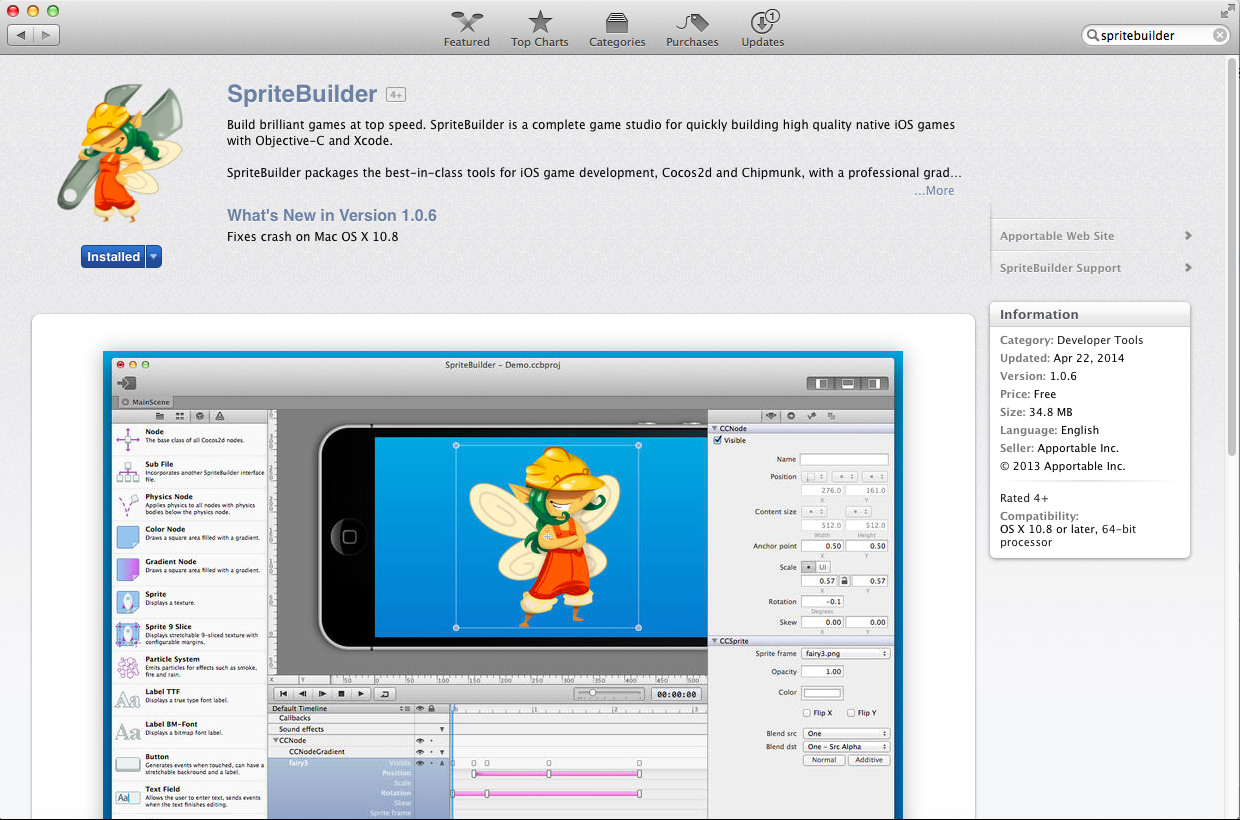
\includegraphics[width=200pt]{images/cocos2d/setup/mac_appstore_install.png}     
		\caption{\cocos{} Technology Stack}
\end{figure}

After a couple of minutes the \SB{} installation should be completed. Later
throughout this chapter you will learn how to set up your first project.

\section{Why \cocos{}}
Well, now you have already installed \cocos{}. I still want to spend a moment on
discussing why we are using this tool. The main goal of \cocos{} is to make
mobile game development \textit{easier}. Earlier we have discussed the basic
concepts and benefits of game engines. You should now know that there are many
problems developers have faced while developing games, animations, physics, etc.
- and most of them have been solved and put into frameworks. You should not
spend your precious time trying to solve them again. So now that you know that
you definitely should use a framework - \textbf{which ones are available and why
should you choose \cocos{}}?

\textit{Add brief discussion on different frameworks}

\section{Introduction to \cocos{}}
First let us take a look at the features of \cocos{}. That will give you a basic
understanding of which tasks you will hand off to the framework, later on we
will be discussing all of these features in detail:
\begin{description}
  \item[Scene Graphs] \cocos{} provides the concepts of scenes and nodes.
  Everything that is rendered to the screen is part of a hierarchical
  \textit{scene graph}. Instead of performing custom drawing code you define
  what your scene looks like by providing a scene graph and \cocos{} will render
  it for you.
  \item[Rendering Engine] When using \cocos{} you don't need to write your own
  rendering code. \cocos{} provides a rendering engine built on top of OpenGL
  ES.
  \item[Action System] A sophisticated action system allows you to define
  movements of objects and animations instead of writing a lot of custom code.
  \item[Physics Engine] The \cocos{} physics engine automatically
  calculates movements of objects, collisions and more.
  \item[Node Library] \cocos{} provides a large set of nodes as part of the
  framework. Nodes can be used to represent images, UI elements, solid colors,
  etc.
\end{description}

There are many more features - but this brief outline shows the most
important ones and should give you an idea why almost all game developers these
days use game engines.  Let's take a closer look at how \cocos{} works.

\subsection{The \cocos{} technology stack}

\cocos{} is built on top of OpenGL ES 2.0. If you have ever written OpenGL code
before, you know that it takes a lot of code even to render the most primitive
scenes.	OpenGL is a fairly low level framework that gives the graphics
programmer a lot of control over how and when certain tasks are performed -
more control then you need for most 2D games. \cocos{} abstracts all of these
tasks for you. Many \cocos{} developers write entire games without writing any
OpenGL code at all. The following diagram shows which technologies are used by
\cocos{}:

\begin{figure}[H]
		\centering
		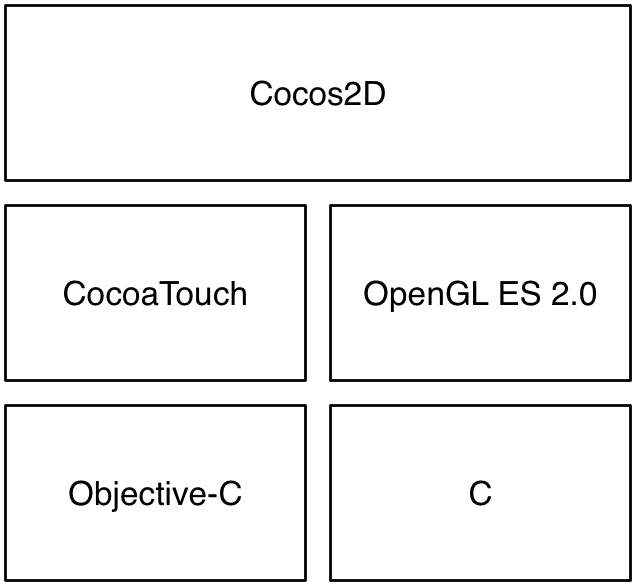
\includegraphics[width=120pt]{images/cocos2d/TechnologyStack.png}     
		\caption{\cocos{} Technology Stack}
\end{figure}

The goal of a game engine like \cocos{} is that the game developer doesn't have
to get in touch with rendering at all. Instead a developer defines which scenes
exist in a game, which objects are part of these scenes and which size, position and appearance these objects have and \cocos{} 
will use OpenGL to render these scenes for him. 

In order to provide this functionality \cocos{} consists of variety of classes -
some important ones will be discussed in this chapter. All \cocos{} classes use the \textit{CC} prefix (\ccscene{}, \ccnode{}, etc.).

When working with a 2D game engine for the first time you will be introduced to
a whole set of new terminology. We have already talked about nodes and scenes
but we haven't discussed what these terms mean. We will now start discussing the
most important terms and get to know how the concepts behind them are
implemented in \cocos{}.

\subsection{Scenes}
Scenes are the basic building blocks of all \cocos{} games, they are the
highest level on which game content can be structured. Each scene in \cocos{} is
a full-screen canvas. For every full-screen section of your game you will use
\textit{one} scene.
\textbf{Add screenshots here}
Here's an example from the MakeGamesWithUs game \textit{Deep Sea Fury}:
% add image
You can see that the game consists of the start scene, the gameplay scene and
the game over scene.

Scenes are represented by the \ccscene{} class. Another
important \cocos{} class for scene handling is \ccdirector{}. The \ccdirector{}
class is responsible for deciding which scene is currently active in the game
(\cocos{} only allows one active scene at a time). Whenever a developer wants to
display a scene or transition between two scenes he needs to use the
\ccdirector{} class.

This means creating and displaying a new scene is a two step process:
\begin{enumerate}
\item Create a new instance of \ccscene{}
\item Tell the \ccdirector{} to display this new scene
\end{enumerate}

You will learn a lot more about this down the road, but the important bottom
line is: \textit{Scenes are the highest level of structure in your game and a
class called \ccdirector{} decides which scene is currently displayed}.

\subsection{Nodes}
Everything that is visible in your \cocos{} game (and a couple of invisible
objects) are \textit{nodes}. Nodes are used to structure the content of a scene.
Every node can have other nodes as its children. \cocos{} provides a huge amount
of different node types. Every node type is a subclass of \ccnode{}.

Most nodes are used to represent an object on the screen (an image, a solid
color, an UI element, etc.), a few other nodes are only used to group other
nodes. All nodes have a size, positions and children (and many other properties
which are less important for us right now). Here are some of the popular
node types of \cocos{}:

\begin{description}
  \item[CCSprite] represents an image or an animated image. Used for characters,
  enemies, etc.
  \item[CCColorNode] a node being displayed in one plain color.
  \item[CCLabelTTF] a node that can represent text in any TTF font.
  \item[CCButton] a interactive node that can receive touches.
\end{description}

Nodes and their children form a scene graph. The concept of a scene graph isn't
unique to \cocos{} it is a common concept of 2D and 3D graphics. A scene graph
is a hierarchy of many different nodes. 

\subsection{Scene Graphs}
Let's take a look at simple example of a scene graph:

\begin{figure}[H]
		\centering
		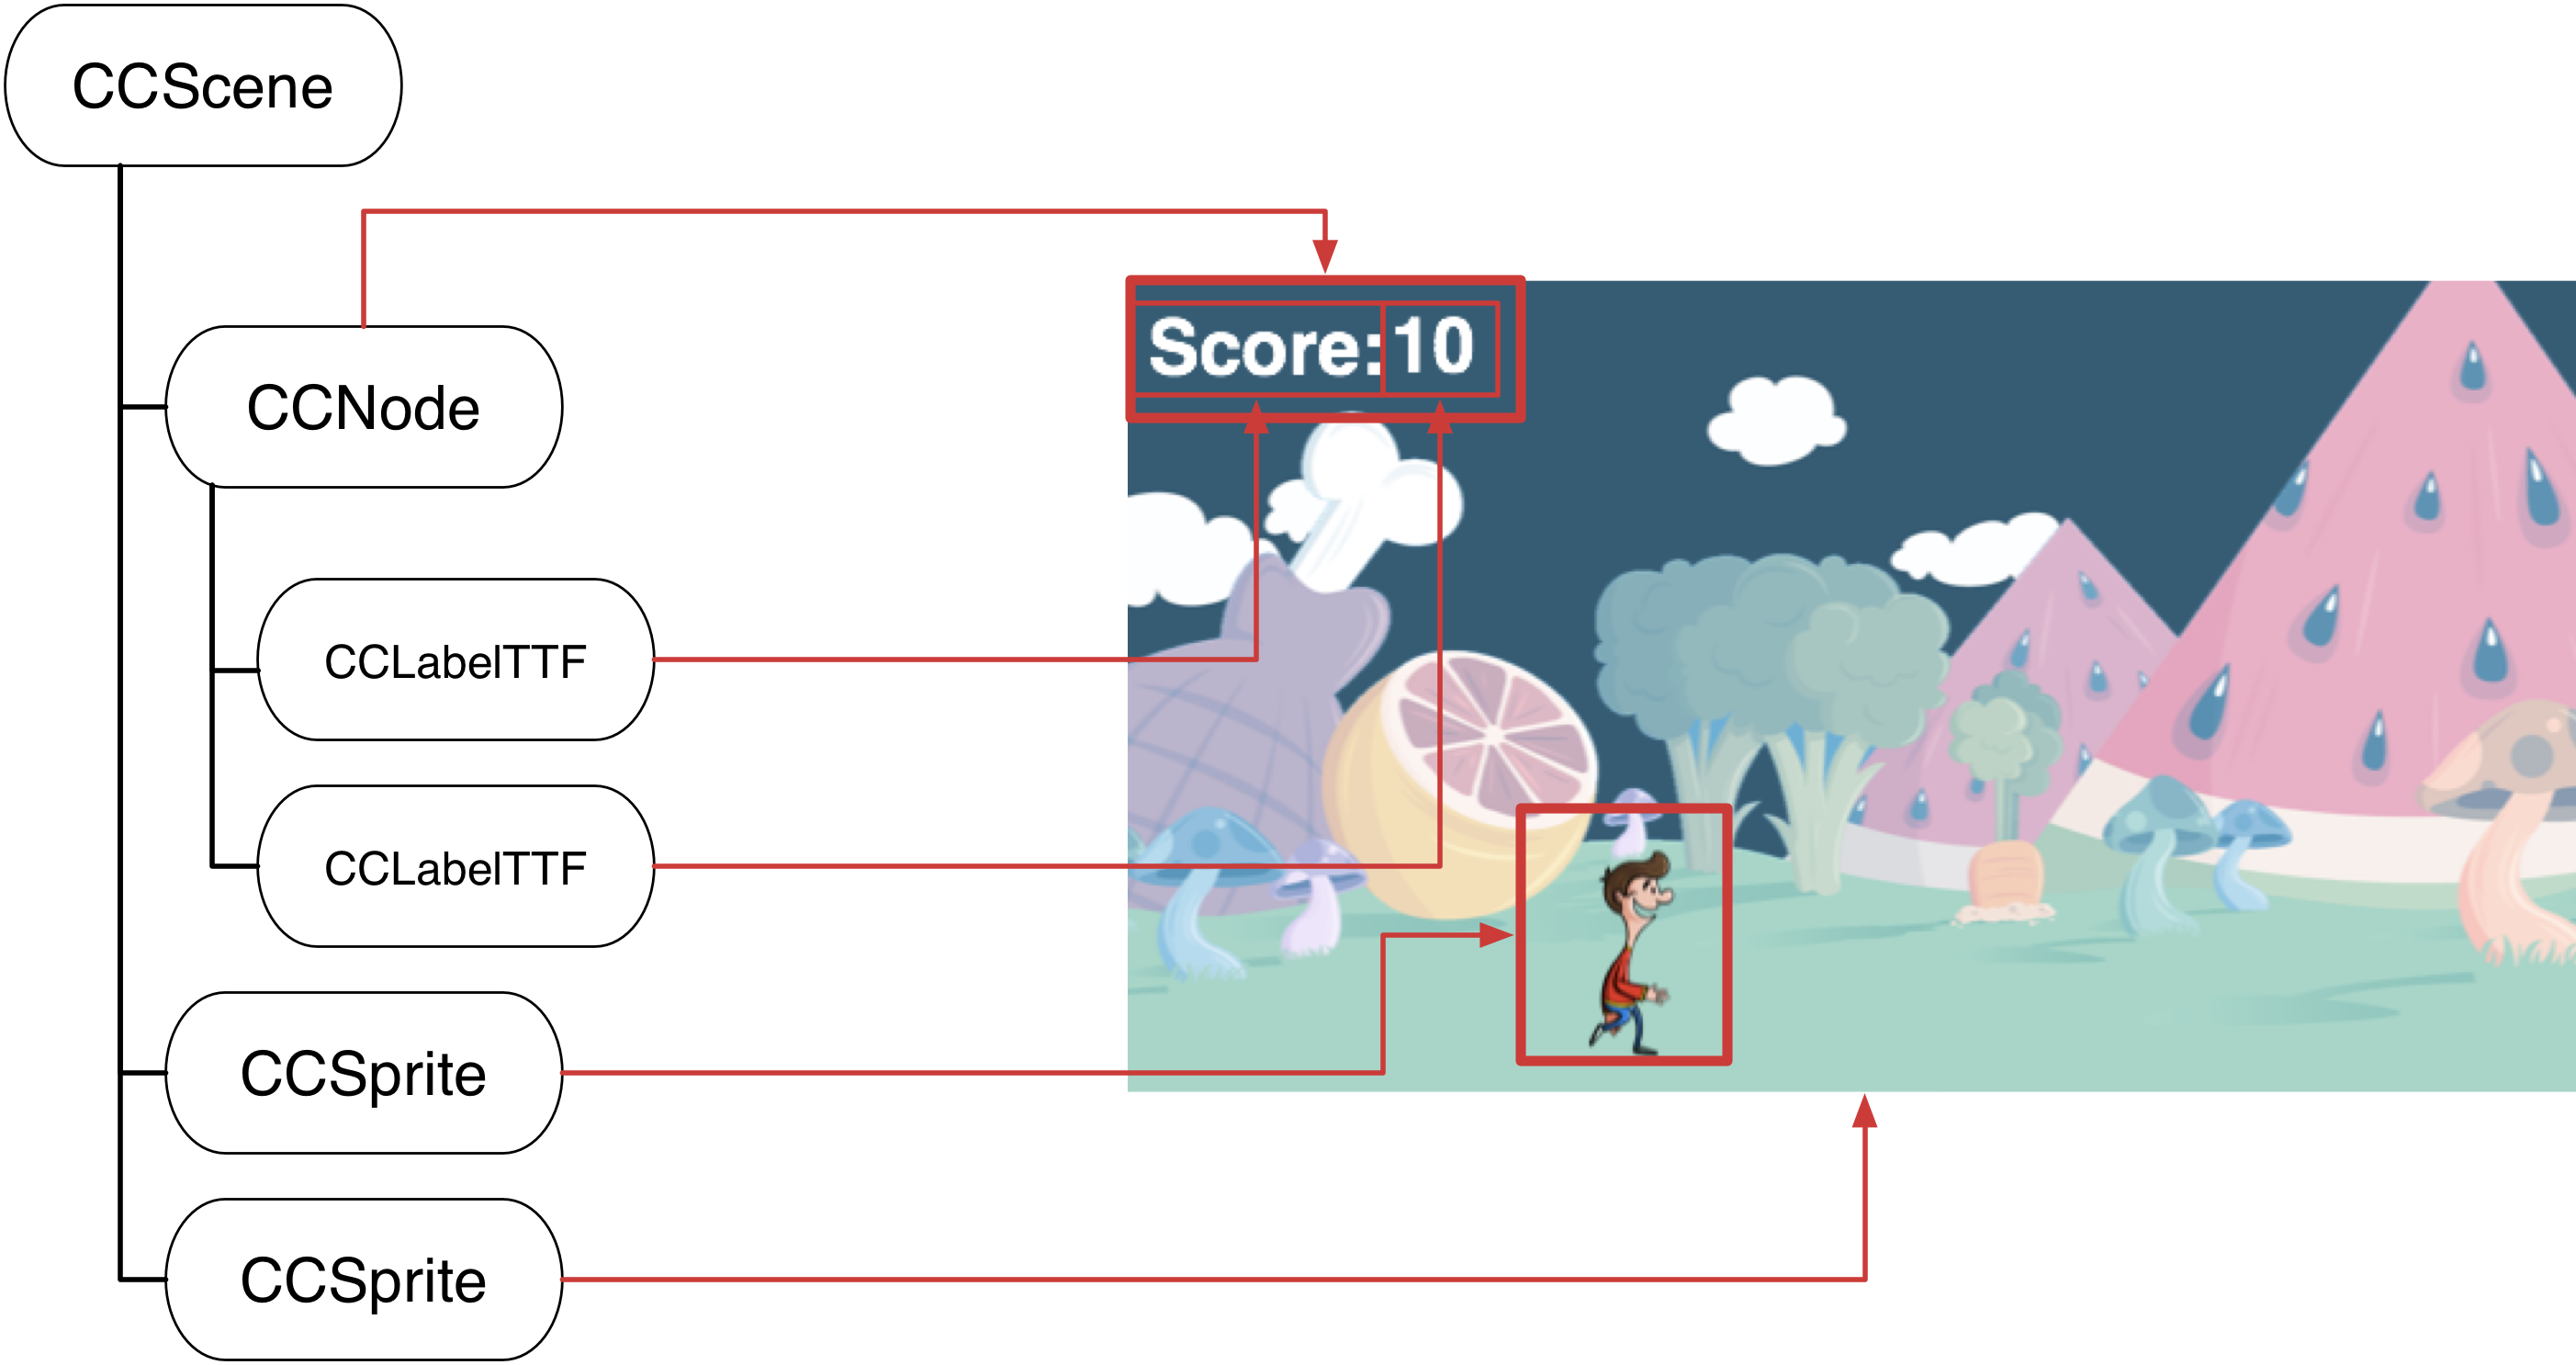
\includegraphics[width=0.9\linewidth]{images/cocos2d/SceneGraph.png}     
		\caption{\cocos{} Scene Graph}
\end{figure}

On the left side of the image you can see the node hierarchy. On the first level
you have the \ccscene{}. As the first child we have a \ccnode{} with two
children of type \cclabel{}. This \ccnode{} is the first example of a grouping
node, it groups the score caption label and the label displaying the actual
score. Instances of \ccnode{} don't have any appearance they are solely used to
group other nodes. Throughout this book you will learn that it often makes sense
to group nodes under certain parent nodes. The main reason is that all children are placed
\textit{relative} to their parents. So if we would want to move the scoreboard
of the example above to the top right corner we would only have to move the
parent node instead of both child nodes. As you can imagine this becomes
even more relevant in games that have ten or more entries in their scoreboard.

\begin{bestpractice}[frametitle={Structuring Nodes}] 
Always group nodes that logically belong together under one parent node. That
will save you a lot of time when you change the layout of your scene.
\end{bestpractice}

The other two objects in the scene graph are simpler. One represents the
background image the other one the main character.

For some games, scene graphs can get very complex and include hundreds of
different nodes. The key takeaways for now are:

\begin{enumerate}
  \item Every node in \cocos{} can have children
  \item A hierarchy of nodes is called a scene graph
  \item Children of nodes are placed relative to their parents - often it is
  useful to group nodes that are moved together under one parent
\end{enumerate}

As you can see nodes are the most important building block of \cocos{} games -
they are used to build everything that is visible in your game. Because it
is so important to understand how nodes work in \cocos{} we will take a look at
the most important properties and methods that \ccnode{} provides.

\subsection{An Introduction to CCNode}
Every visible object in your game will be a subclass of \ccnode{}. Because
you use nodes to build and arrange your scenes it is important to understand
how nodes are positioned and how positions of nodes can be accessed. Let's
discuss the most relevant properties and methods to access and change
size and position of a \ccnode{}:

\begin{description}
\item[contentSizeInPoints] the size of this node in points
\item[positionInPoints] the position of this node in points, expressed relative
to the parent of this node
\item[anchor point] the anchor point is the center point for rotations and the reference point for positioning this node
\item[boundingBox] the bounding box is a rectangle that encloses a node. You can
only read it but not set it
\end{description}

The \textit{contentSizeInPoints} and \textit{positionInPoints} properties
express the size and the position of a \ccnode{} and should be fairly easy to
understand. The \textit{bounding box} and the \textit{anchor point} however, are
concepts related to game development and these may be new to you. The bounding
box is a rectangle that encloses the entire node, you will see an example of a
bounding box in the next diagram. The anchor point is relevant for positioning
and rotating nodes.

Let's take a look at how anchor points influence positioning first. We know that
the position of a node is expressed relative to its parent. More specifically every node position in
\cocos{} is expressed from the \textit{position reference corner} of the parent
to the anchor point of the \ccnode{}. Here's a visual example in which a bear
node is placed relative to a background node:

\begin{figure}[H]
		\centering
		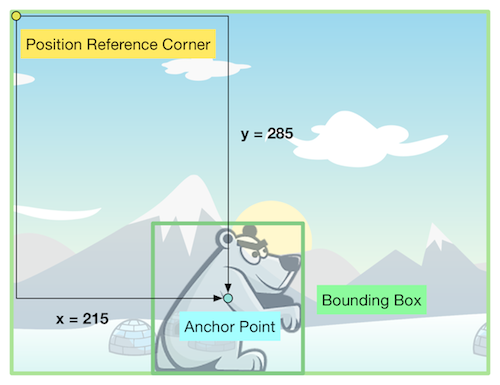
\includegraphics[width=0.5\linewidth]{images/cocos2d/ccnode/NodePositioning.png}     
		\caption{\ccnode{} positioning example}
\end{figure}

As you can see, the \textit{anchor point} and the \textit{position reference
corner} influence the position of a node. The anchor point can have any value
between (0, 0), representing the bottom left corner of a node and (1,1),
representing the top right corner of a node. In the example above, the bear has
a anchor point of (0.5, 0.5) which is at the center of the bear. By choosing an
anchor point of (0.5, 0.5), the \textit{center} of the bear will be positioned
at (215, 285). If we would choose an anchor point of (0,0) the \textit{bottom
left} corner of the bear would be positioned at (215, 285).

The \textit{position reference
corner} lets us define from which of the four corners of the parent node we are
expressing the position of a node. In the example above the top left corner is
the \textit{position reference corner}. We will discuss how to use position reference corners when we start 
creating games that shall work on multiple screen sizes.

The anchor point is not only important for the positioning of a node. It has a
second important function - it represents the center of rotation for a
\ccnode{}. Every \ccnode{} rotates around its own anchor point. Here's an
example of rotating the bear node with two different anchor points:

\begin{figure}[H]
		\centering
		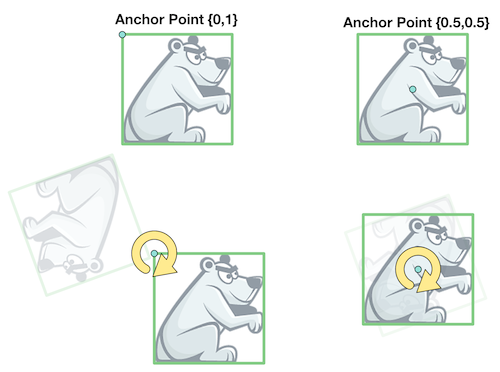
\includegraphics[width=0.6\linewidth]{images/cocos2d/ccnode/Rotation.png}     
		\caption{\ccnode{} positioning example}
\end{figure}

There is a lot more to learn about \ccnode{}, but for now our only goal is to
get a basic understanding of how \cocos{} games are structured and what the most
important parts of \cocos{} are.

You now know that \cocos{} game are structured into scenes. You know that
everything visible in your game is a \ccnode{} and that every \ccnode{} can have
multiple children. You also got a basic understanding of how nodes are
positioned in \cocos{}.

Now that you have that basic understanding, we will take a look at a second tool which we will be using throughout this book: \SB{}.

\section{Introduction to \SB{}}
You have learned the fundamentals of the game engine we will use. Now we will
take a look at a tool called \SB{} which we will use to create the majority of
our game content. The main purpose of \SB{} is to provide a visual editor for
the creation of scenes, animations and more. For most games you will create some
basic mechanics in code (enemy movement, score mechanism, etc.) but you will create
 most of your game content in \SB{} since it is a lot easier to create
levels, menus and other scenes in an editor that provides you with a live
preview instead of putting these scenes together in code.

If you have never used \SB{} before, it is very important to understand that
everything that can be implemented in \SB{} can also be implemented in code.
\SB{} is not part of the game engine, it just allows you to configure \cocos{}
scenes and nodes in an editor instead of configuring them in code.

\subsection{Creating a first project}
To dive into the features of \SB{} we will create our first project! 
Create a new project by opening SpriteBuilder and selecting \textit{File > New >
Project...}:
\begin{figure}[H]
		\centering
		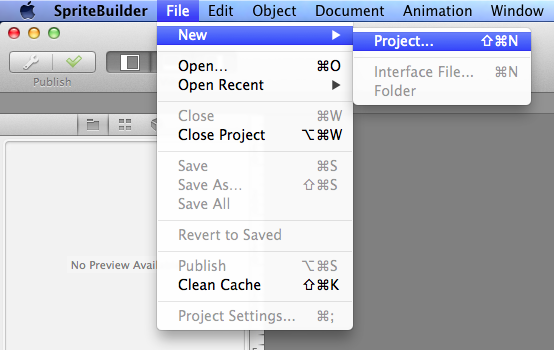
\includegraphics[width=0.9\linewidth]{images/cocos2d/setup/spritebuilder_new_project.png}     
\end{figure}

\SB{} will ask for a name and a location for the new project. Name it
\textit{HelloSB}. After you create the project the folder structure should look similar to this:
\begin{figure}[H]
		\centering
		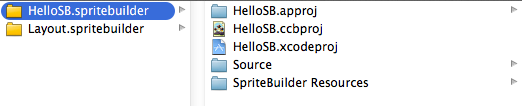
\includegraphics[width=250pt]{images/cocos2d/setup/project_structure.png}     
		\caption{\SB{} project folder structure}
\end{figure}

Every \SB{} project is contained in a \textit{.spritebuilder} folder. Within
this folder all the files of the \SB{} project are stored - along with an \xcode{}
project. 

\begin{lamp}[frametitle={\SB{} and Xcode}] 
\SB{} will create an \xcode{} project for every new project you create! The
\xcode{} project will automatically contain the newest version of \cocos{} -
very handy.
\end{lamp}

Later on you will learn more about how the \SB{} project and the \xcode{}
project work together. The general rule is that all code will be part of the
\xcode{} project and most content creation will happen in the \SB{} project.

\subsection{The Editor}
When you have created your first \SB{} project you will see that the \SB{} UI
gets enabled. Let's take a look at the different parts of the editor to get a
better understanding of \SB{}.

The \SB{} interface is divided into 4 main sections:
\begin{figure}[H]
		\centering
		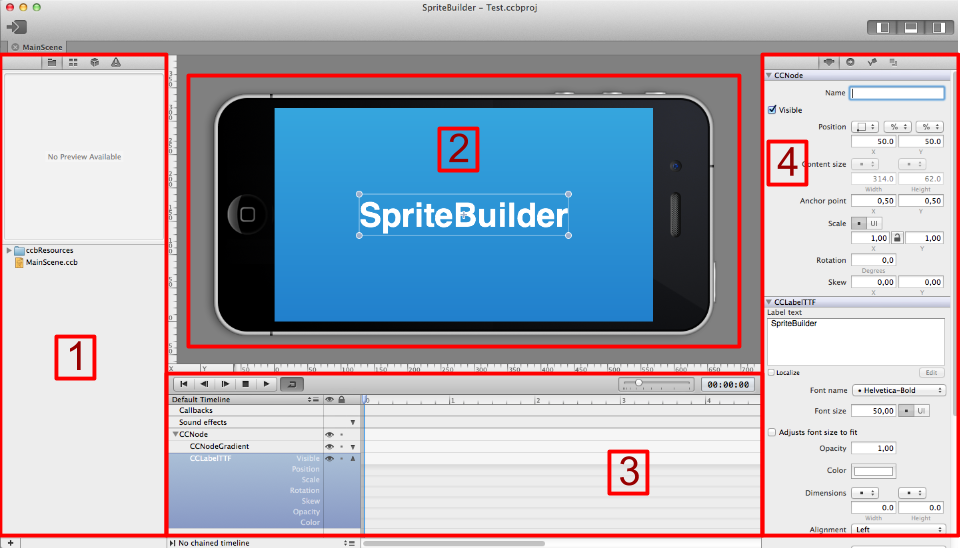
\includegraphics[width=0.9\linewidth]{images/spritebuilder/spritebuilder_ui.png}     
\end{figure} 
\begin{enumerate}
  \item \textit{Resource/Component Browser:} Here you can see the different
  resources and scenes you have created or added to your project. You can also select different types of Nodes and drag them into your scene.
  \item \textit{Stage:} The stage will preview your current scene. Here you can
  arrange all of the nodes that belong to a scene. 
  \item \textit{Timeline:} The timeline is used to create animations within
  SpriteBuilder.
  \item \textit{Inspector:} Once you select a node in your scene, this detail
  view will display a lot of editable information about that node. You can modify positions, content (the text of a label, for example) and physics properties.
\end{enumerate}
Let's take a closer look at some of the most important views.

\subsubsection{File View}
The first tab in the resource/component browser represents the \textit{File
View}.
It lists all the \textit{.ccb} files and resources that are part of the \SB{}
project:
\begin{figure}[H]
		\centering
		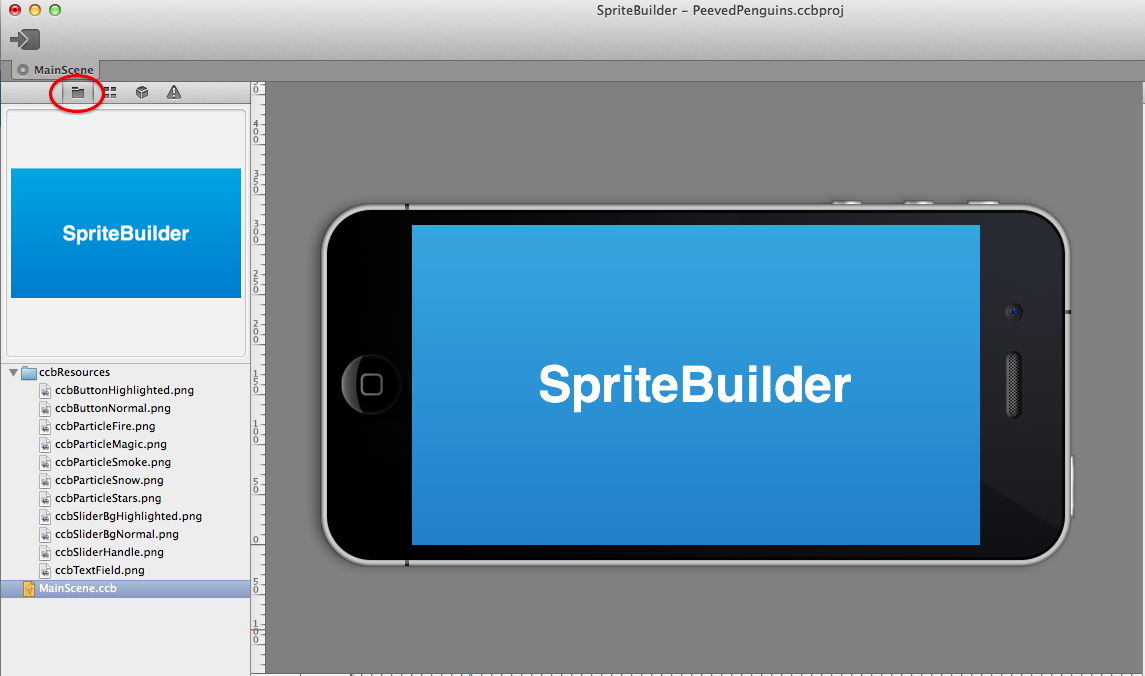
\includegraphics[width=0.8\linewidth]{images/spritebuilder/spritebuilder_fileview.png}     
\end{figure} 
In this view you can add new resources and restructure your project's folder
hierarchy.
\subsubsection{Node Library}
The third tab in the left view is the {Node Library}:
\begin{figure}[H]
		\centering
		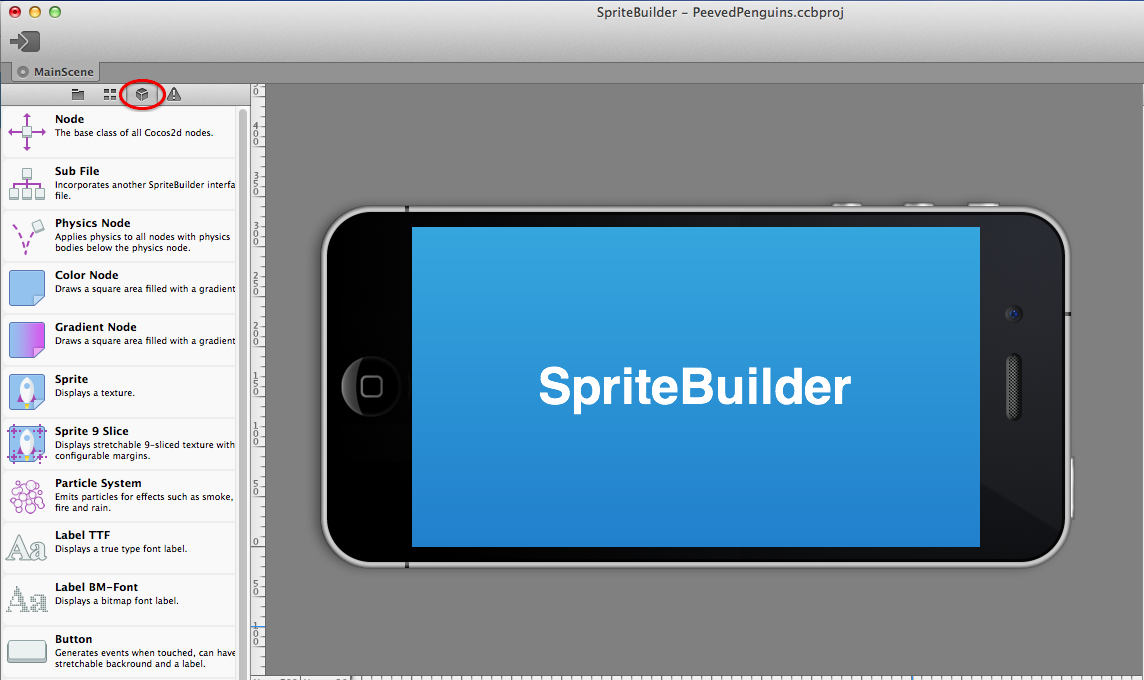
\includegraphics[width=0.8\linewidth]{images/spritebuilder/spritebuilder_nodeview.png}     
\end{figure} 
This panel shows you all available node types you can use to construct your
Gameplay scenes and menus. You will drag these nodes from this view to the stage
in the center to add them to your scenes.

\subsubsection{Inspector}
The first tab of the Detail View (the right panel) is
the Inspector. Once you have selected an object on your stage you can use this panel to modify many of its properties, like position and color:
\begin{figure}[H]
		\centering
		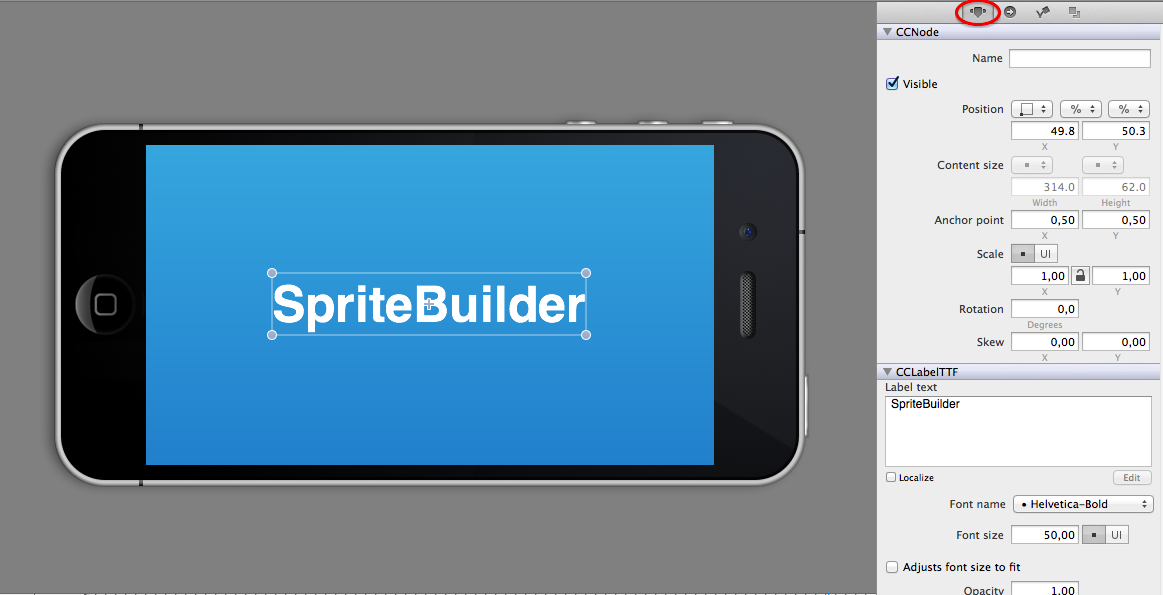
\includegraphics[width=0.8\linewidth]{images/spritebuilder/spritebuilder_inspector.png}     
\end{figure} 

\subsubsection{Code Connections}\index{Code Connections} 
The second tab on the right panel let's you manage code connections for your
selected node. As mentioned previously the entire code for your games will be
written as part of the \xcode{} project. This view allows you to create
connections between the \xcode{} project and the \SB{} project. For example you can set a custom Objective-C class for a node or you can select
a method in your code that shall be called once a button in your scene is tapped. 

\begin{figure}[H]
		\centering
		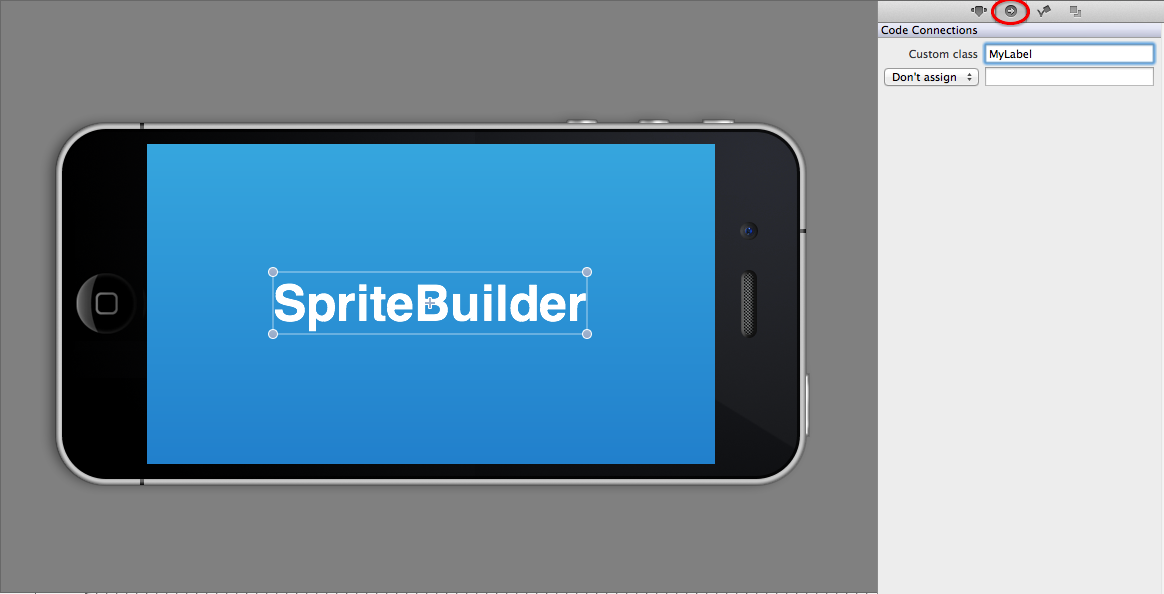
\includegraphics[width=0.8\linewidth]{images/spritebuilder/spritebuilder_codeconnections.png}     
\end{figure} 
Code connections will be discussed in detail later on.

\subsection{\ccbfile{}s}
\ccbfile{}s are the basic building blocks of your \SB{} project. Every scene in
your game that is created with \SB{} is represented by one \ccbfile{}. However
\ccbfile{}s are not only used to create entire scenes - they are used to create
any kind of scene graph. \SB{} provides different kinds of templates depending
on which type of scene graph you want to create. You get an overview of the
available \ccbfile{} templates when you create a new one, by selecting
\textit{New > File... } from the \textit{File} menu in \SB{}:
\begin{figure}[H]
		\centering
		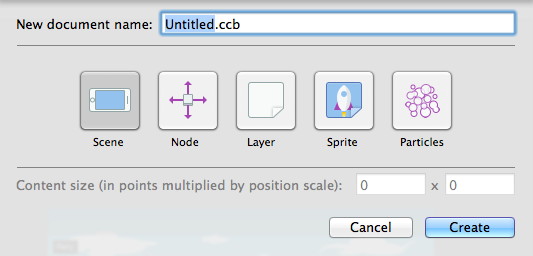
\includegraphics[width=240pt]{images/spritebuilder/new-ccb.png}     
\end{figure} 
These are the different templates briefly explained:
\begin{description}
\item[Scenes] will fill the full screen size of the device.
\item[Nodes] used primarily for grouping functionality, don't have a size.
\item[Layers] are nodes with a content size. This is useful, for instance, when
creating levels or contents for scroll views.
\item[Sprites] used to create (animated) characters, enemies, etc.
\item[Particles] is used to design particle effects.
\end{description}
You will get a good understanding when to use which type of \ccbfile{} once we
get started with our example projects. The key takeaway is that \ccbfile{}s are
used by \SB{} to store an entire scene graph including size, positions and many
other properties of all the nodes that you have added.

\subsection{How \SB{} and \xcode{} work together}
\label{Publish}
I have mentioned how \SB{} and \xcode{} integrate a couple of times briefly. In
order to be a well versed and efficient \SB{} game developer it is very
important to understand the details of this cooperation.

When creating a \SB{} project, \SB{} will create and maintain a corresponding
\xcode{} project. In \SB{} will you create multiple \ccbfile{}s that describe
the content of the scenes in your game. You will also add the resources that
you want to use in your game and set up code connections to interact with the
code in your \xcode{} project. \xcode{} will be the place where you add code to
your project and where you run the actual game.

Since \xcode{} is the tool that actually compiles and runs your game it needs
to know about all the scenes and resources that are part of your \SB{} project.
Therefore \SB{} has a \textbf{publish}\index{publish} functionality, provided by
a button in the top left corner of the interface:
\begin{figure}[H]
		\centering
		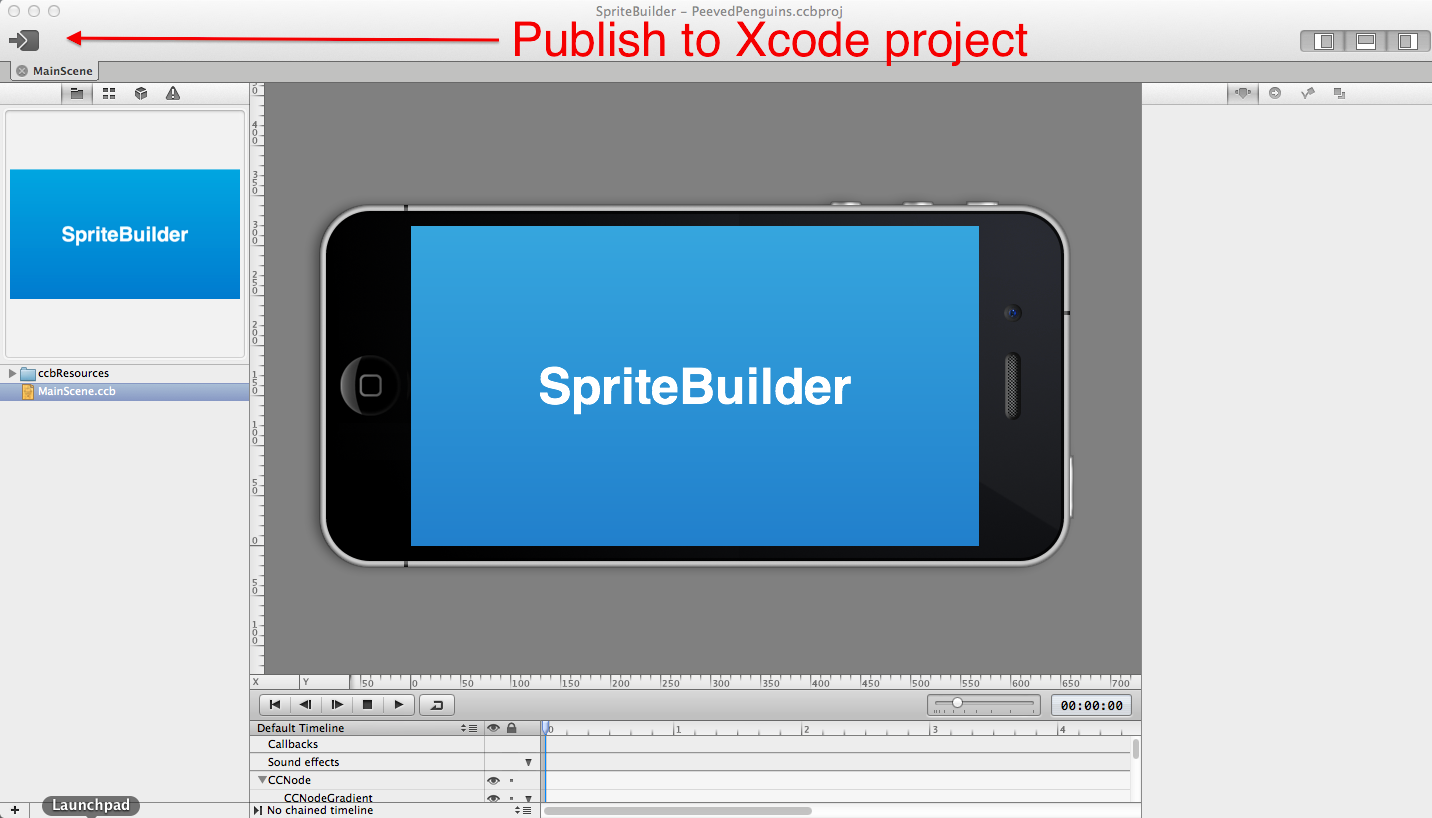
\includegraphics[width=0.9\linewidth]{images/spritebuilder/spritebuilder_publish_button.png}
		\caption{Use the publish button to update your \xcode{} project with the
		latest changes in your \SB{} project.}
		%\label{labelstruct} 
\end{figure}
Using that button, you publish your changes in your
\SB{} project to your \xcode{} project. Whenever you changed your \SB{}
project and want to run it you should hit this button before building the \xcode{}
project.

Here's a diagram that visualizes how \SB{} and \xcode{} work together:
\begin{figure}[H]
		\centering
		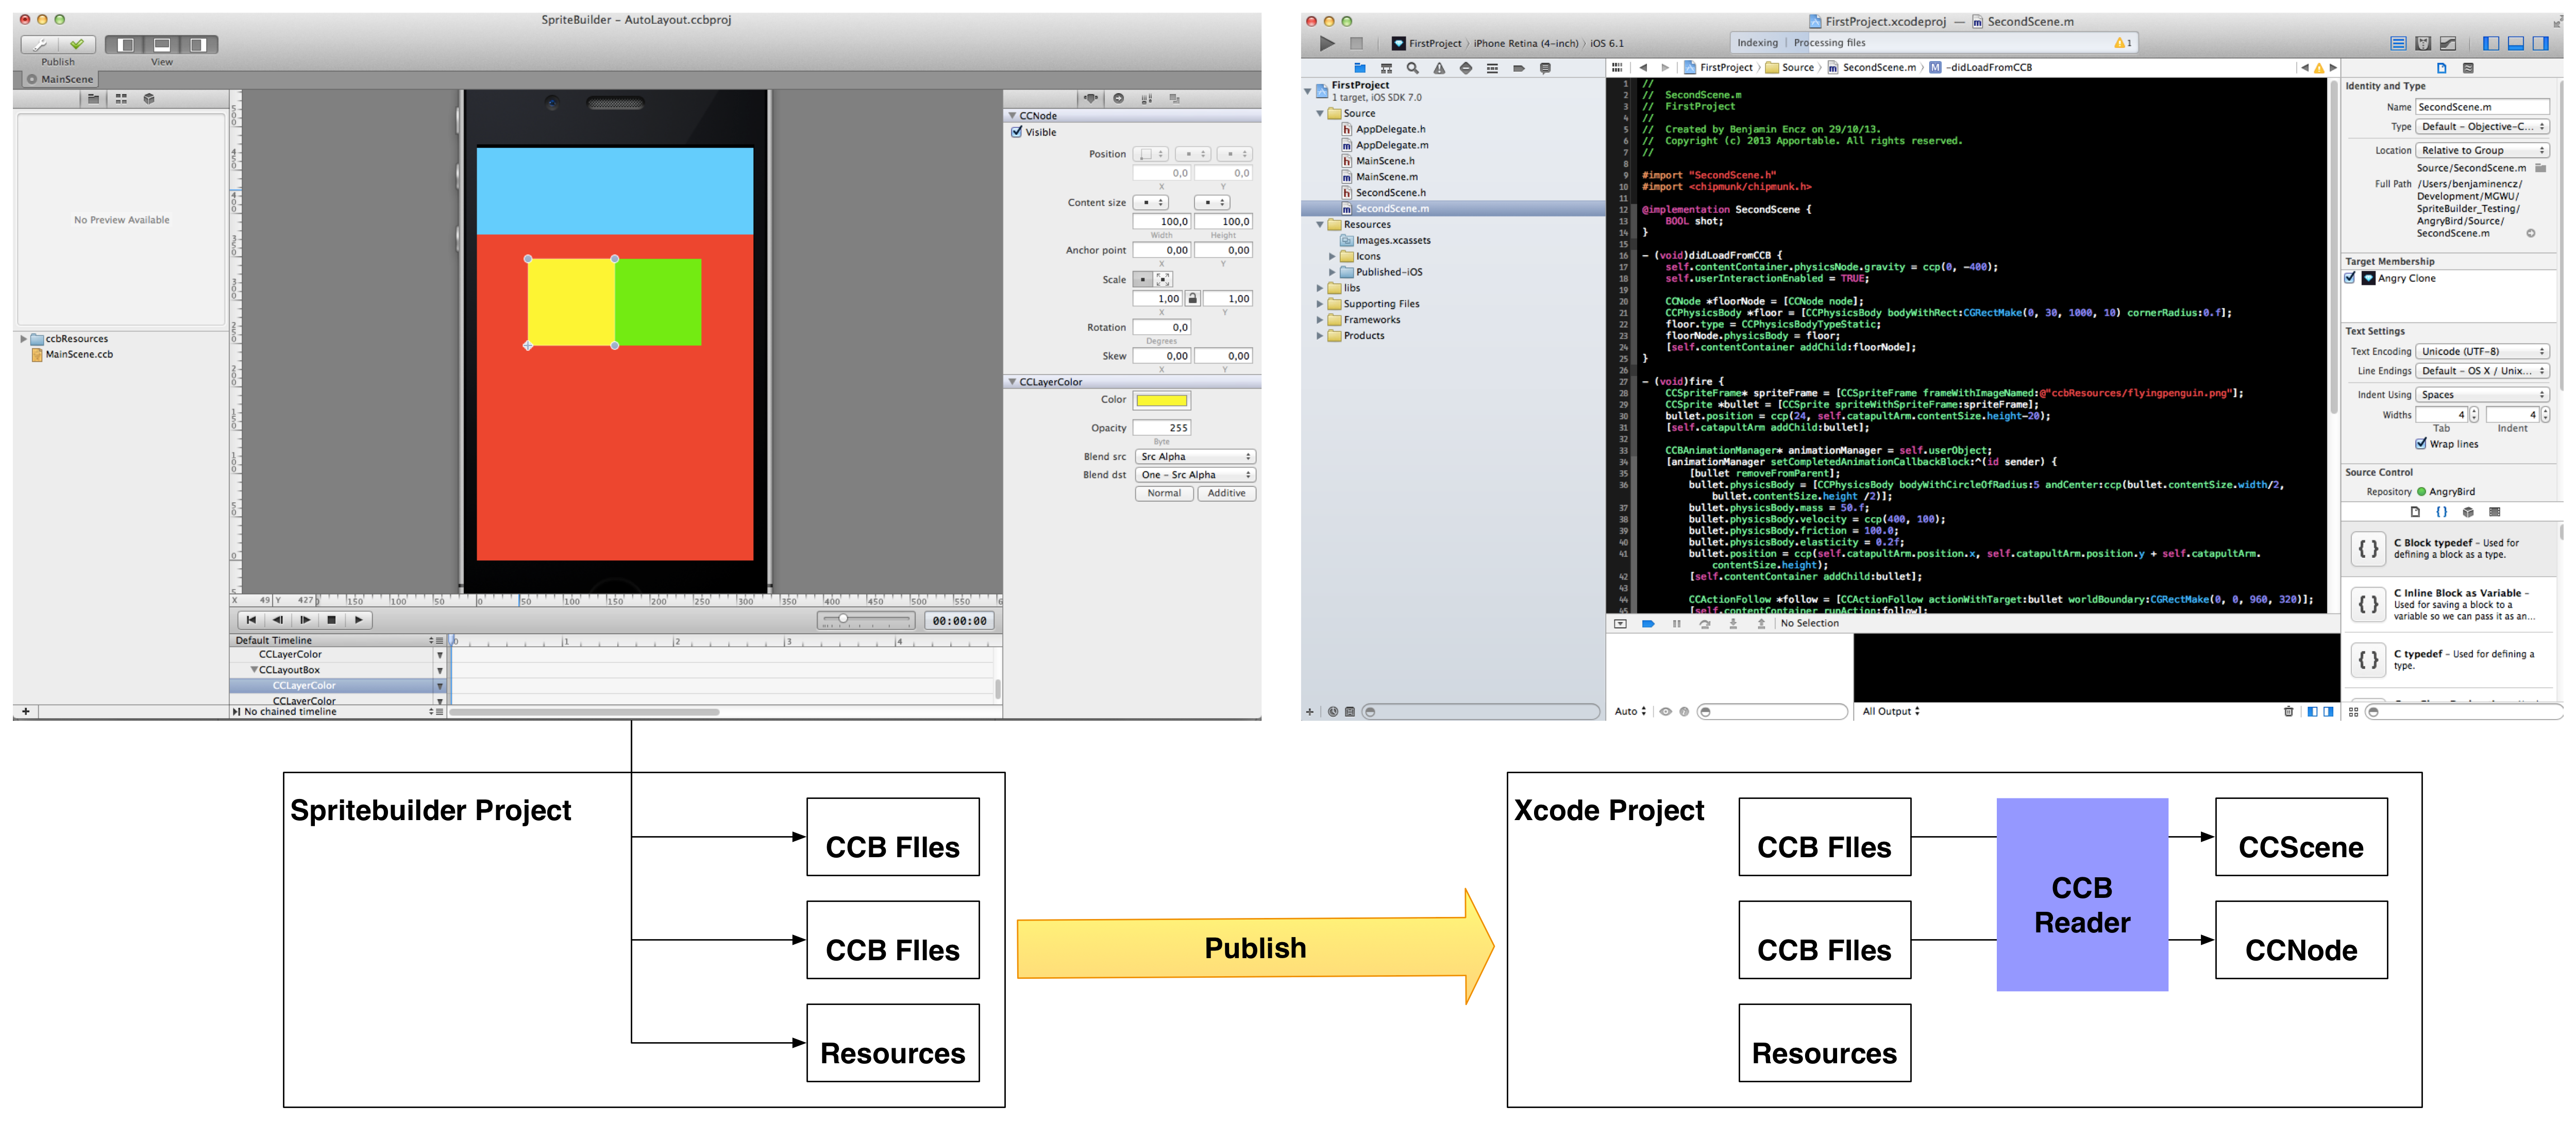
\includegraphics[width=0.9\linewidth]{images/spritebuilder/spritebuilder_publishing.png}
		\caption{\SB{} creates and organizes a \xcode{} project for you. Adding
		all the resources and scenes you have created.}
		%\label{labelstruct} 
\end{figure}
\ccbfile{}s created in \SB{} store a scene graph; the hierarchy and positions of
your nodes. When publishing a \SB{} project the \ccbfile{}s and all other
project resources are copied to your \xcode{} project.
\label{CCBReader}
When running the project in \xcode{} a class called CCBReader will parse your
\ccbfile{}s and create the according \ccnode{} subclasses to reconstruct the scene
graph you have designed in \spriteb{}.

If you would use \cocos{} without \SB{} you would manually create instances of
\ccnode{}, \ccsprite{}, etc. in code and add children to these nodes -
essentially building the entire scene graph in code.

When using \SB{} the CCBReader class will build this scene graph for you, based
on the information stored in the \ccbfile{}s that you created in \SB{}.

Another important part of information contained in \ccbfile{}s that we have not
discussed in detail yet are \textit{Code Connections}.

\subsection{Code Connections}
\label{CodeConnections}
Code connections are used to create links between your scenes in \SB{} and your
code in \xcode{}. There are three basic types of code connections:
\begin{description}
\item[Custom Classes] are an important information for the CCBReader. As
mentioned previously the CCBReader builds the scene graph by creating different
nodes based on the information in your \ccbfile{}. By default it will create an
instance of \ccsprite{} for every sprite you added in \SB{} an instance of \ccnode{} for every node you added, etc. Often
however you will want to add custom behaviour to a node (for example a movement
pattern for an enemy). Then you will have to use the \textit{Custom Class}
property to tell the CCBReader which class it should instantiate instead of the
default one. Whichever class you enter here needs to be a subclass of the
default class (e.g. a subclass of \ccsprite{}). You will learn how to use this
feature in the final project of this chapter!
\item[Variable Assignments] If you have assigned a \textit{Custom Class} you can
use variables assignments to retrieve references to different nodes in the
scene. For example a character might want a reference to its right arm node (a
child of the character node) in order to move it. 
\item[Callbacks] are only available to UI elements like buttons and sliders.
They allow you to decide which method should be called on which class once a
button is pressed.
\end{description}
Now you should have an idea about what code connections are used for and which
kinds exist. We will discuss the details of all types when we use them as part
of our example projects.

\section{A first \SB{} project} 
You have already created the \SB{} project called \textit{HelloSB}. Now we will
start adding some content to it. The project built in this chapter will consist
of two scenes one start screen and one game screen. In the game screen the user will be able to spawn randomly
colored squares that rotate, by tapping on the screen.
\begin{figure}[H]
		\centering
		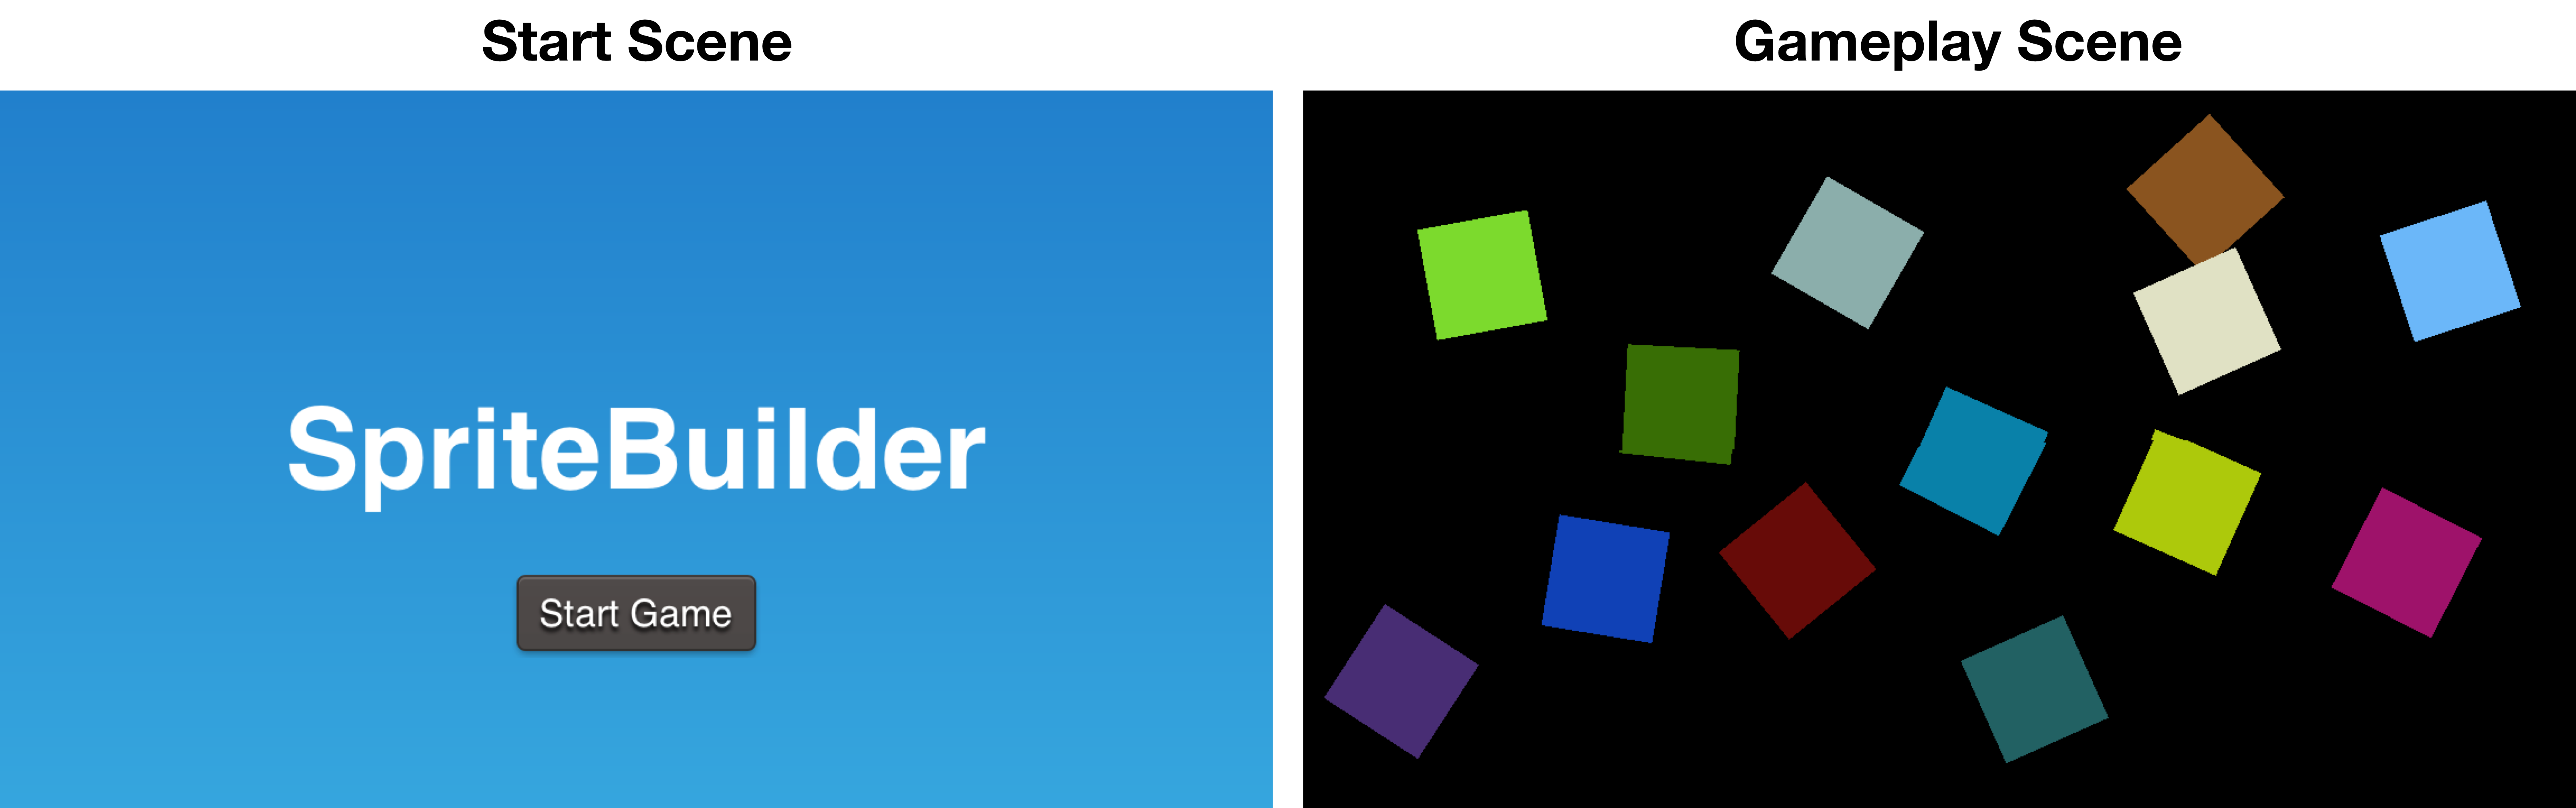
\includegraphics[width=0.9\linewidth]{images/firstproject/first_project.png}
		\caption{The project build throughout this chapter}
		%\label{labelstruct} 
\end{figure}
By creating this project you will learn all of the following:
\begin{itemize}
  \item Creating scenes in \SB{}
  \item Creating code connections (callbacks, variable assignments and custom
  classes)
  \item Switching between different scenes
  \item Manipulate a scene graph from code (add/remove nodes, load CCB Files and
  add them to the scene)
  \item Use the \cocos{} action system to create animations
  \item Use the \cocos{} touch handling system to capture touches
\end{itemize}

\subsection{Setting up the first scene}
%explain code connections in detail here
Now it is time to open the \textit{HelloSB} \SB{} project. We want to add a
\textit{Start Button} to the first scene. When this button is tapped we want to
switch to the second scene. 

\subsubsection{Positioning the first button}
Start by adding a button to the first scene:

\begin{figure}[H]
		\centering
		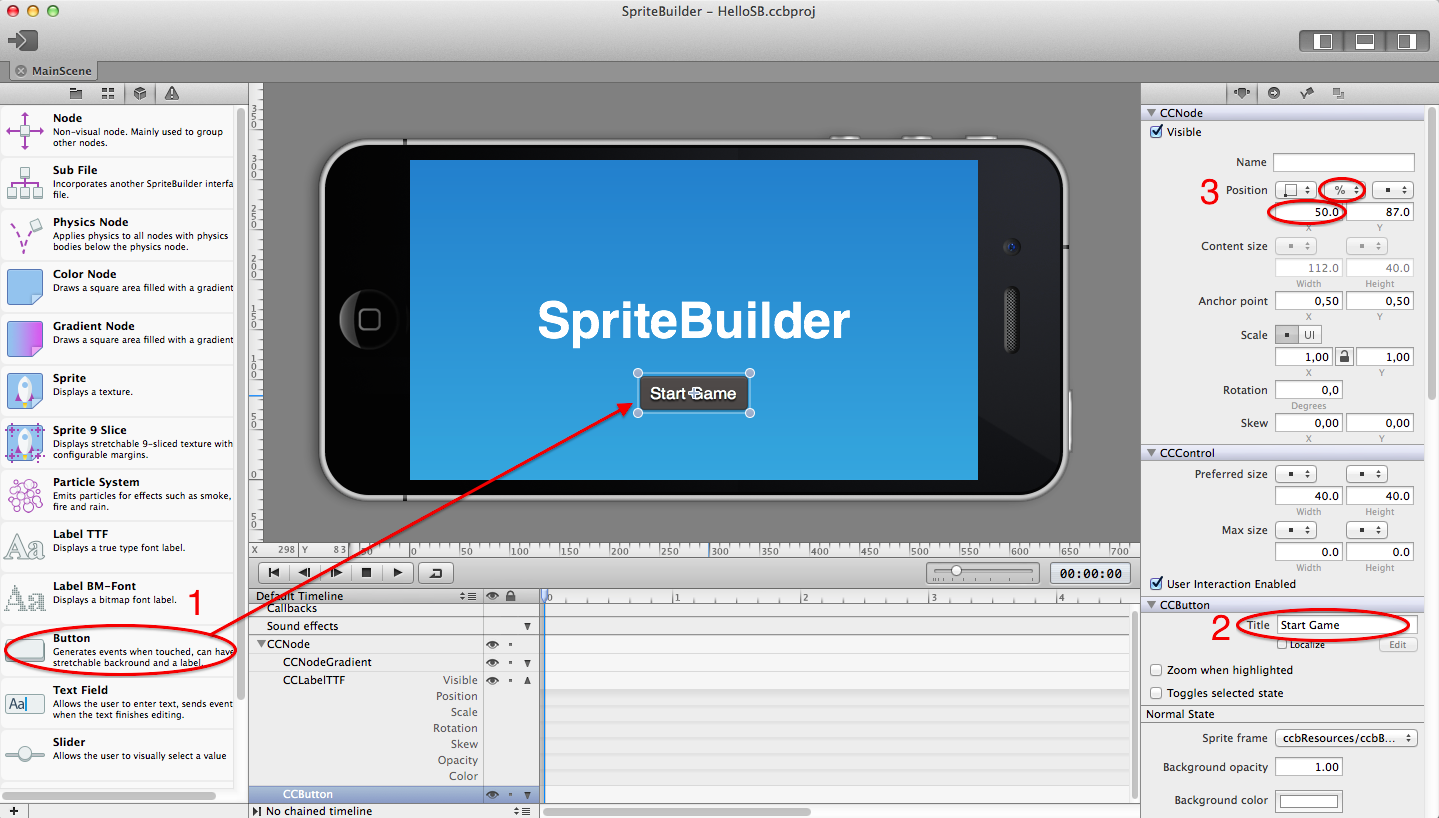
\includegraphics[width=0.9\linewidth]{images/firstproject/add_button.png}
		\caption{The project build throughout this chapter}
		%\label{labelstruct} 
\end{figure}

One simple button, but since this is your first action in \SB{} there's
\textit{lots} to explain about it. Let's look at the three steps highlighted in
the image above, one by one.

\begin{description}
\item[(1)] Open \textit{MainScene.ccb} by double clicking it in the left
resource pane. Then open the third tab in the left pane, the \textit{Node
Library}. Remember, this section shows you all the different node types
supported by \SB{}. Select the \textit{Button} and drag it over to the stage,
dropping it below the existing label. Dropping it on the stage will add this
node to your scene. Another way of adding a node to a scene is dropping it to
the timeline at the bottom of the screen - we will look at this later.
\item[(2)] Make sure the button is selected, because we want to change some
properties of it. Whenever you have selected a node the right pane will display
all the properties you can edit. Navigate to the \textit{Title} textfield in the
property pane and change the title of the button to \textit{Start Game}.
\item[(3)] So far - so simple. Step number three will expose you to a very
interesting feature of \SB{}: the positioning system. It will allow you to not
only use absolute positions but also positions that are relative to the size of
the parent node. We want to center the button horizontally so we choose the
position type for the X component to be \textit{in percent of parent
container} by selecting that option from the dropdown menu. Now we assign
\textit{50} as value, because that expresses the horizontal center of the parent
container. Whichever screen this button will be displayed on, it will always be
vertically centered (yes, even on an iPad)!
\end{description}

\begin{details}[frametitle={Positioning System in \cocos{} and \SB{}}] 
The positioning system in \cocos{} is designed from the ground up to make it
easy to design scenes and user interfaces for different screen sizes and
resolutions. The comfortable days where the 3.5-inch iPhone was the only 
available iOS device and defining layouts with absolute positions was acceptable
are finally over. Today app and game developers face a variety of different
devices and customers justifiably expect your software to work great on all of
them. \cocos{} offers the following properties on \ccnode{}s to allow developers
to design their interfaces with great flexibility:

\begin{itemize}
  \item Anchor Point
  \item Reference Corner
  \item Position Type
  \item Size Type
\end{itemize}

Check the extra chapter on dynamic layouts in \SB{}. %TODO: Add reference, etc.

\end{details}

Now the button is placed correctly. Next, we want to assign an action to it.
When the button is tapped we want to transition to our second scene.

\subsubsection{Setting up a code connection}

Earlier you learned that \SB{} has three types of code connections 
(\ref{CodeConnections}). Now we will use one of them in our project -
\textit{Callbacks}\index{Code Connections!Callbacks}. Callbacks are only
available to nodes that allow for some sort of user interaction (this means they need to be subclasses of
\inlinecode{CCControl}). Buttons, next to Sliders and Text Fields are one of
these types of nodes. Select the button we have added to the scene earlier and
select the third tab of the right pane:

\begin{figure}[H]
		\centering
		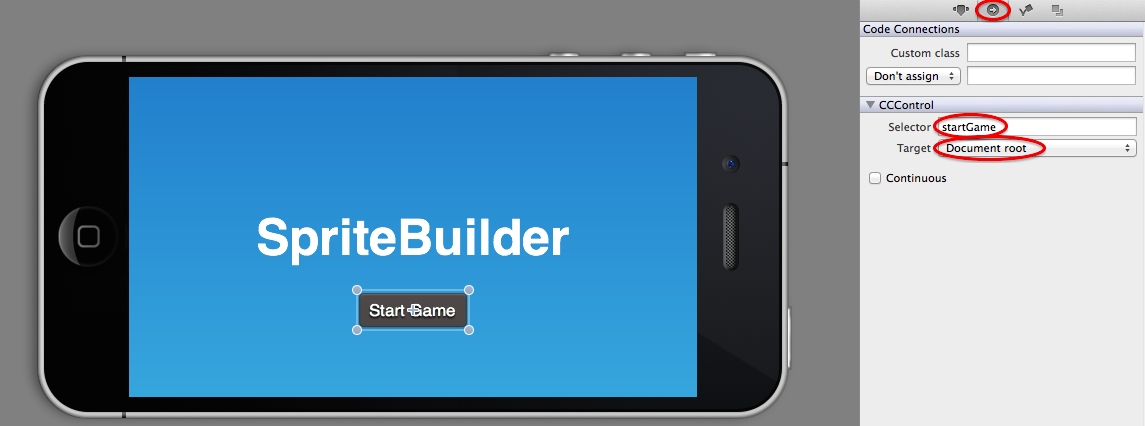
\includegraphics[width=0.9\linewidth]{images/firstproject/button_callback.png}
		\caption{Nodes that allow user interaction can use callback methods to
		connect to the code base}
		%\label{labelstruct} 
\end{figure}

Inside the CCControll section you can see two options called \textit{selector}
and \textit{target}. Here you can choose which method (selector) shall be
called on which object (target) when this button is tapped by a user. As
selector enter \inlinecode{startGame}. As target choose \textit{Document Root}.

\begin{details}[frametitle={Targets and Selectors}] 
The concept of targets and selectors is part of design pattern widely used
throughout the Cocoa framework (Target/Action pattern). A \textit{selector} is
a method name and a \textit{target} is the object that shall receive this method.
Further reading:
\url{https://developer.apple.com/library/ios/documentation/general/conceptual/Devpedia-CocoaApp/TargetAction.html}
\end{details}

As you can see you cannot choose an arbitrary object to be the target of this
callback, you can only choose between two different ones:
\begin{description}\label{DocumentRoot_Owner}
\item[Document Root] The document root\index{Document Root} is the highest node
within the current \ccbfile{}. The hierarchy of the \ccbfile{} is shown in the
\SB{} timeline: \begin{figure}[H]
		\centering
		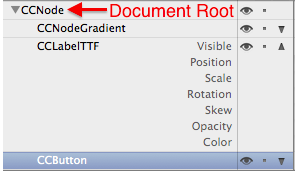
\includegraphics[width=150pt]{images/firstproject/documentroot_node.png}
		%\label{labelstruct} 
\end{figure}
If you select the document root as target, the \inlinecode{startGame} method
will be called on the top level \ccnode{}. 
\item[Owner] if you want the callback to call an object that is not part of your
\ccbfile{} you can use the \textit{owner} option. Later in this book you will
learn how to set up an owner object for a \ccbfile{}.
\end{description}

For our button we have decided that the \inlinecode{startGame} method should be
called on the document root when the button is tapped. Next, we will have to
implement this \inlinecode{startGame} method within our document root. But to
which \textit{class} could we add this method? In order to find that out we need to understand the
concept of \textit{Custom Classes} \index{Code Connections!Custom Classes}.
Think about it - by default our document root is an instance of a plain
\ccnode{} class.
Now we want to call a method called \inlinecode{startGame} on this object. Our
problem: the \ccnode{} class does not have a \inlinecode{startGame} method! This
is where custom classes come to rescue us, they allow us to tell \SB{} that our
document root node should \textbf{not} be a plain \ccnode{} but should be an
instance of a class that we have created and that knows about our
\inlinecode{startGame} method. To define a custom class for the document root
you need to select the document root (the top-level \ccnode{}) from the timeline
and open the third tab in the right pane:

\begin{figure}[H]
		\centering
		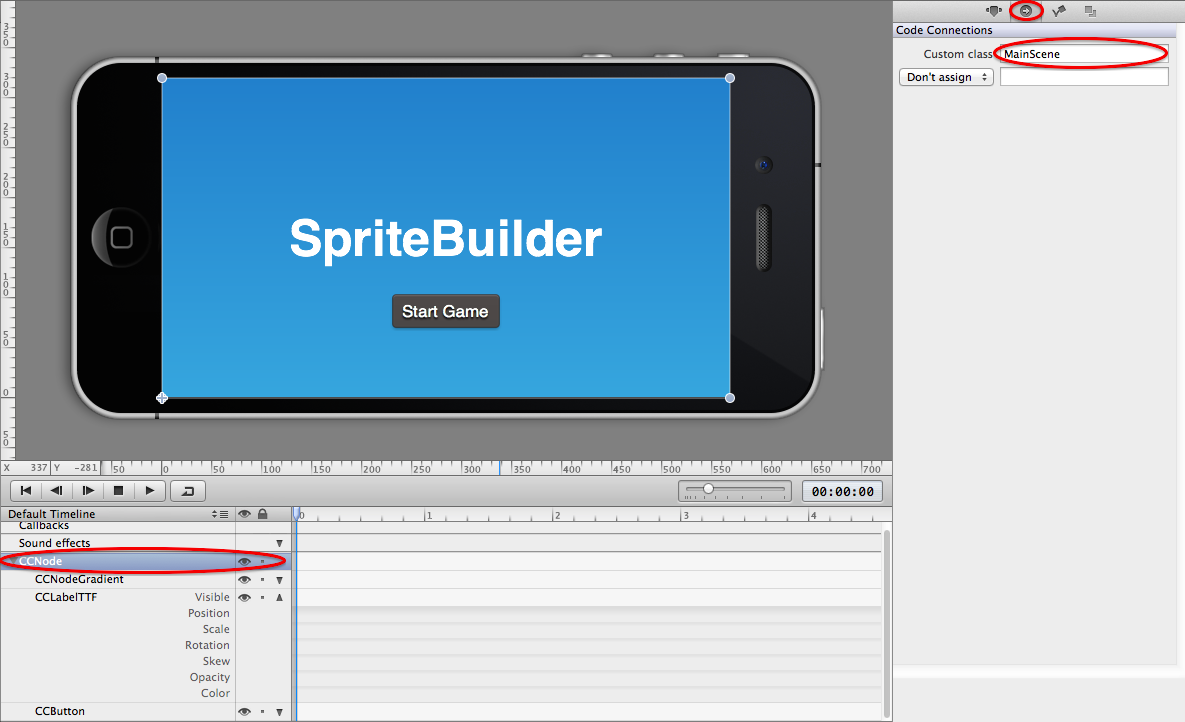
\includegraphics[width=0.9\linewidth]{images/firstproject/custom_class.png}
		%\label{labelstruct} 
\end{figure}

In the \textit{Custom class} textfield a developer can enter a class name. The
class entered here needs to be part of the \xcode{} project related to this
\SB{} project. As you can see every new \SB{} project already comes with a
custom class set up for the root node of \textit{MainScene.ccb}. When the
CCBReader loads this \ccbfile{} it will create an instance of \inlinecode{MainScene} instead of an instance of
\inlinecode{CCNode}.
Now our document root object is a \inlinecode{MainScene} object! That also means
that we have saved the puzzle of where to add the code for the
\inlinecode{startGame} method - it needs to be part of the
\inlinecode{MainScene} class.

\begin{details}[frametitle={Requirements for Custom Classes}] \index{Code
Connections!Custom Classes}
Every custom class has to be a subclass of the default class for a given node.
For example, the default class for the \textit{Sprite} node in \SB{} is
\ccsprite{}. If a developer wants to set a custom class for a Sprite node, that
class has to be a subclass of \ccsprite{}. \textbf{Why?} \SB{} expects custom
classes to only \textbf{add} behaviour to a default class. All the functionality
of the default class should remain available. If your custom class for a Sprite
node doesn't allow \SB{} to set an image, because it is a subclass of \ccnode{}
the CCBReader and finally also you will run into big problems!
\end{details}

\subsubsection{Adding Code to a \SB{} project}
When creating games with \SB{} we are always working with two tools. \SB{} to
create interfaces and scenes (our game content) and \xcode{} to add code (game
mechanics, etc.). Now we will add our first few lines of code to the
\inlinecode{MainScene} class. Now it's time to publish the changes in our \SB{}
project, so that they are available in our \xcode{} project. Use the publish
button in the top left corner of the \SB{} interface (\ref{Publish}). 

Now open the \xcode{} project (it's called \textit{HelloSB.xcodeproj} and is
located inside the \textit{HelloSB.spritebuilder} folder). You will see that
project contains two classes, \inlinecode{AppDelegate} and
\inlinecode{MainScene}. As part of the template for new \SB{} projects the
\inlinecode{MainScene} class has already been created for you. For any
subsequent custom classes you link in your \SB{} project you will need to create
the according class in \xcode{} on your own. 

Now it's finally time to implement the \inlinecode{startGame} method. Open the
\textit{MainScene.m} and file and add the following method:

\begin{lstlisting}
- (void)startGame {
  CCLOG(@"Start Button Pressed!");
}
\end{lstlisting} 

For now we will simply use the \inlinecode{CCLOG} macro to log a text to the
console once the button is pressed, this is an easy way to check if our code
connection is set up correctly.

\begin{lamp}[frametitle={Displaying the console in \xcode{}}] 
To display the console in \xcode{} select \textit{View -> Debug Area ->
Activate Console}.
\end{lamp}

Now, run the \xcode{} project by hitting the play button in the top left corner.
You should check that you have selected \textit{HelloSB} as target and are set
up to run the app on a simulator (indicated by a device description instead of
a device name):
\begin{figure}[H]
		\centering
		
\includegraphics[width=200pt]{images/firstproject/run_app.png}
\end{figure}
Hitting the run button will compile your app and launch it on an iOS simulator.
Once your app is launched, click on the start button and check the console for
the log message. You should see something similar to this:

\begin{figure}[H]
		\centering
		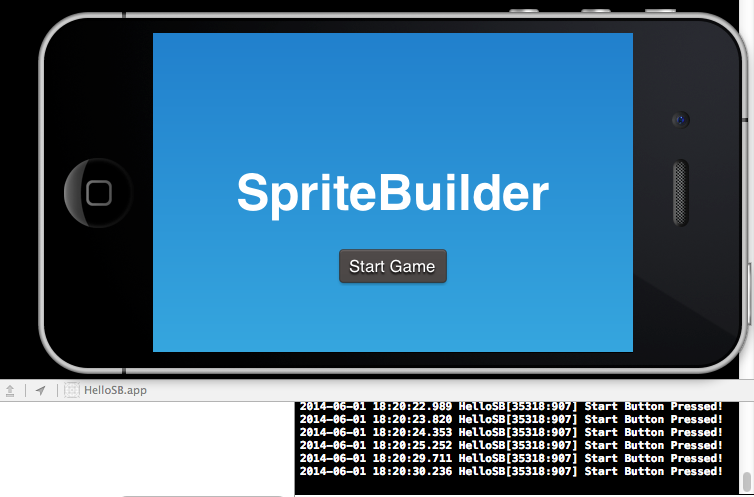
\includegraphics[width=0.9\linewidth]{images/firstproject/button_success_log.png}
		%\label{labelstruct} 
\end{figure}

You have successfully set up your first \SB{} scene and have created a working
code connection! Later on this button shall trigger a transition to the second
scene in the game. Before we can implement that we need to create the second
scene in our \SB{} project!

%TODO: potentially ad recap of how custom class works?

\begin{error}
If you are not getting the expected result, check for all of these common
errors:
\begin{itemize}
  \item Have you published your \SB{} before running in \xcode{}?
  \item Is the custom class of the root node of \textit{MainScene.ccb} set to
  \inlinecode{MainScene}
  \item Does the button in \textit{MainScene.ccb} have the correct target and
  selector?
\end{itemize}
\end{error}

\subsection{Creating the Gameplay Scene}
Now it's time to create your first scene using \SB{} from scratch. The scene we
are going to create is the Gameplay scene. To create a new scene (or any
other \ccbfile{}) select: \textit{File -> New -> File\ldots} from the \SB{} menu.
Then you will see the following dialog appear:

\begin{figure}[H]
		\centering
		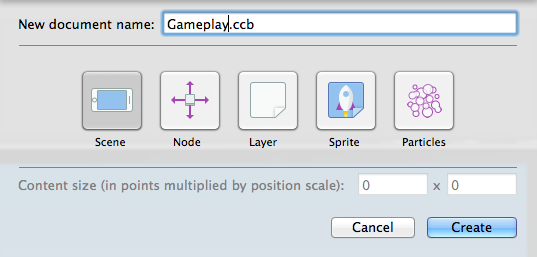
\includegraphics[width=250pt]{images/firstproject/new_scene.png}
		%\label{labelstruct} 
\end{figure}

The dialog will ask you for a name for the \ccbfile{} and a template type. For
now we are going to use the name \textit{Gameplay.ccb} and the type
\textit{Scene}. Once you hit the create button you will see the new, blank
scene appear.

Our Gameplay scene will remain empty. As you have seen in the outline
of the project, we want to dynamically add colored objects to the game, whenever
the user taps into our Gameplay scene - initially however, the scene will be
blank. Now that we have created the Gameplay scene, we can add the transition
from the Main scene to the Gameplay scene.

\subsection{Adding a Scene Transition}
Transitions \index{Scene Transition} are essential for any game. We use them
whenever we want to switch from one scene to another. Transitions cannot be configured in
\SB{}, they always need to be implemented in code. To implement this step,
you need to open your \xcode{} project again.

\cocos{} has one central class that is responsible for displaying the active
scene and generating transitions between different scenes:
\inlinecode{CCDirector}\index{CCDirector}. CCDirector is implemented as a
singleton - thus there's only one CCDirector per \cocos{} game. The instance can be accessed
through the class method \inlinecode{[CCDirector sharedInstance]}.

\begin{lamp}[frametitle={CCDirector is versatile!}] 
CCDirector is responsible for a lot more than only handling active scenes and
scene transitions. It is basically a collection of different global \cocos{}
settings. The scene handling methods however are the most frequently used
CCDirector methods.
\end{lamp}

CCDirector provides a large collection of methods to present scenes with and
without transitions, here are the most important ones:

\begin{lstlisting}
- (void)presentScene:(CCScene *)scene;
- (void)presentScene:(CCScene *)scene withTransition:(CCTransition *)transition;
- (void)pushScene:(CCScene*) scene;
- (void)pushScene:(CCScene *)scene withTransition:(CCTransition *)transition;
- (void)popScene;
- (void)popSceneWithTransition:(CCTransition *)transition;
- (void)popToRootScene;
- (void)popToRootSceneWithTransition:(CCTransition *)transition;
\end{lstlisting}

\cocos{} has two different approaches for displaying a new scene.
\textbf{Replacing} the current scene with a new one, using the
\inlinecode{presentScene:} methods, or \textbf{Pushing} the new scene on top of
the currently active one using the \inlinecode{pushScene:} methods. Whichever
type you choose, you always have the option to provide a transition effect for
presenting a scene, or not to provide a transition effect and display the new
scene instantaneously. If you want to provide an effect you need to create an
instance of \inlinecode{CCTransition}.

Before we look into using transition effects, let's take a look at the
differences between pushing and replacing a scene.

\subsubsection{Replacing scenes vs. pushing scenes}
When you simply want to replace the current scene with a new one you should use
the \inlinecode{presentScene:} method. Here's an example:
\begin{lstlisting}
[[CCDirector sharedDirector] presentScene:myNewScene];
\end{lstlisting}
Very simple! So why would one use the \inlinecode{pushScene:} method?
Let's assume the following scenario where we want to implement a menu with
multiple submenus. Whenever a player hits the back button, he wants to return
to the previous menu:
\begin{figure}[H]
		\centering
		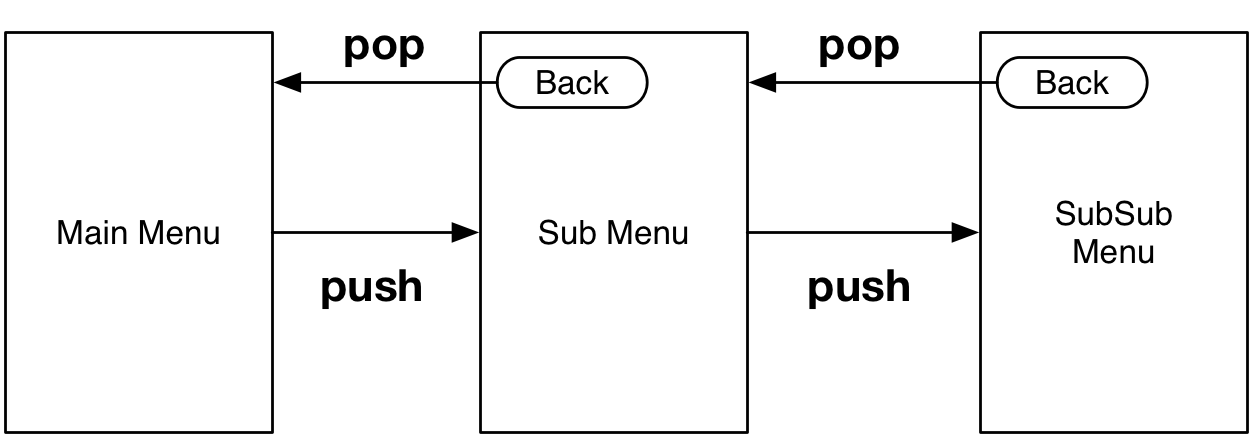
\includegraphics[width=250pt]{images/firstproject/navigation_stack.png}
		%\label{labelstruct} 
\end{figure}
This is a case where it is a lot easier to use \inlinecode{pushScene:} and
\inlinecode{popScene:} instead of simply replacing the currently running scene.
Whenever a player selects a button that opens a sub-menu, we call:
\begin{lstlisting}
[[CCDirector sharedDirector] pushScene:submenu];
\end{lstlisting}
And whenever a player hits the \textit{back} button in one of the sub-menus, we
simply call:
\begin{lstlisting}
[[CCDirector sharedDirector] popScene];
\end{lstlisting}
This works, because CCDirector will remember the scene that we pushed before the
current one and can easily return to it. This concept is called a
\textit{Navigation Stack}.

If you would try to implement the menu hierarchy using
\inlinecode{presentScene:} you would have to explicitly define which scene each
back button will present. The code for the back button of \textit{SubMenu}
would look like this:
\begin{lstlisting}
[[CCDirector sharedDirector] presentScene:mainMenu];
\end{lstlisting}
If you would ever change the menu hierarchy in your game, you would have to
change the code for each back button.

\begin{bestpractice}[frametitle={Scene transitions - the right way}] 
For \textbf{one time transitions} for example from a splash screen to the
gameplay of a game, use \inlinecode{presentScene:}. Whenever a user can navigate
between your scenes, e.g. by using a back button to return to the previous
scene, make use of the navigation stack by using the \inlinecode{pushScene:} and
\inlinecode{popScene:} methods.
\end{bestpractice}

\subsubsection{Adding transition effects}
For every scene replacement method there's one variation that takes an instance
of \inlinecode{CCTransition}. The CCTransition instance provides an animation
for transitions between different scenes. CCTransition provides multiple class
methods to easily create them. Here's an example of how to provide an animated
transition:
\begin{lstlisting}
CCTransition *transition = [CCTransition transitionCrossFadeWithDuration:1.f];
[[CCDirector sharedDirector] presentScene:gameplayScene
withTransition:transition];
\end{lstlisting}

\subsubsection{Implementing a scene transition for our game}
Now that you know the most important details about scene transitions, let's add
the transition from our start scene to our Gameplay scene. Open
\textit{MainScene.m} in \xcode{}. Earlier we have already implemented a test
version of the \inlinecode{startGame} method, where we printed a log message to
the console. Now replace the current implementation of \inlinecode{startGame}
with this one:
\begin{lstlisting}
- (void)startGame {
  CCScene *gameplayScene = [CCBReader loadAsScene:@"Gameplay"];
  CCTransition *transition = [CCTransition transitionFadeWithDuration:1.0];
  [[CCDirector sharedDirector] presentScene:gameplayScene withTransition:transition];
}
\end{lstlisting}
Now that you are familiar with scene transitions, the only interesting line
should be the one where we use the \inlinecode{CCBReader}\index{CCBReader} to
load a \ccbfile{}. The CCBReader class was briefly introduced at the beginning
of this chapter (\ref{CCBReader}). It is capable of reading \SB{}s
\textit{.ccbi} files and creating the according \cocos{} classes from the
information stored in them. Whenever we want to load a scene or any
other type of node that we created in \SB{} into code we use the CCBReader
class. In the lines shown above, we load the content of our
\textit{Gameplay.ccb} into a variable called \inlinecode{gameplayScene}. The
\inlinecode{loadAsScene:} method wraps whatever scene graph you load into an
instance of \inlinecode{CCScene}, use it whenever you want to load a \ccbfile{}
as a scene. %TODO: needs more explanation
Then we create a simple fade transition and store that object in
the \inlinecode{transition} variable. Finally we use the \inlinecode{CCDirector} to present our loaded scene with the transition we just created.

You are now ready to run this version of the game from \xcode{}! When you tap
the \textit{Start} button on the first scene, you should see a transition to our
black Gameplay scene that lasts for one second.

\textbf{Well done!} You have learned how to create a new scene in \SB{} and how
to implement transition between different scenes in a game. Now let's implement
the actual gameplay of our first example game!

\begin{details}[frametitle={.ccb and .ccbi}] 
The files with the file extension \textit{.ccb} are in XML-format and are used
by \SB{} to store and read information about a scene or node created in \SB{}.
When a \SB{} project gets published, \SB{} generates a binary version of
each \textit{.ccb} file. The file extension for these binary files is
\textit{.ccbi} and they are a lot smaller than their corresponding
\textit{.ccb} files. The CCBReader reads these smaller binary files.
\end{details}

\subsection{Implementing the Gameplay}
Now it's time to implement the actual gameplay. For our first project we want to
keep that fairly simple. Whenever a user touches the screen, we want to add a
rotating square with a random color to the gameplay scene. We position the
square at the location of the touch. 

\subsubsection{Creating the Square \ccbfile{}}

Let's start by creating the square we want
to spawn during the game in \SB{}. Create a new \ccbfile{} of type
\textit{Node}: 
\begin{figure}[H]
		\centering
		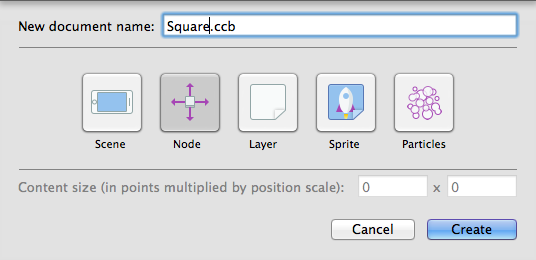
\includegraphics[width=250pt]{images/firstproject/square_ccb.png}
		%\label{labelstruct} 
\end{figure}
The squares we generate in the game shall have a color. A default \ccnode{}
cannot display a color. In order to display a color we need to use a
\inlinecode{CCNodeColor}. The \SB{} node for a CCNodeColor is called
\textit{Color Node}. The root node of every \ccbfile{} is a plain \ccnode{},
that cannot be changed. This means we need to add the \textit{Color Node} as a
child of the root node of \textit{Square.ccb}:
\begin{figure}[H]
		\centering
		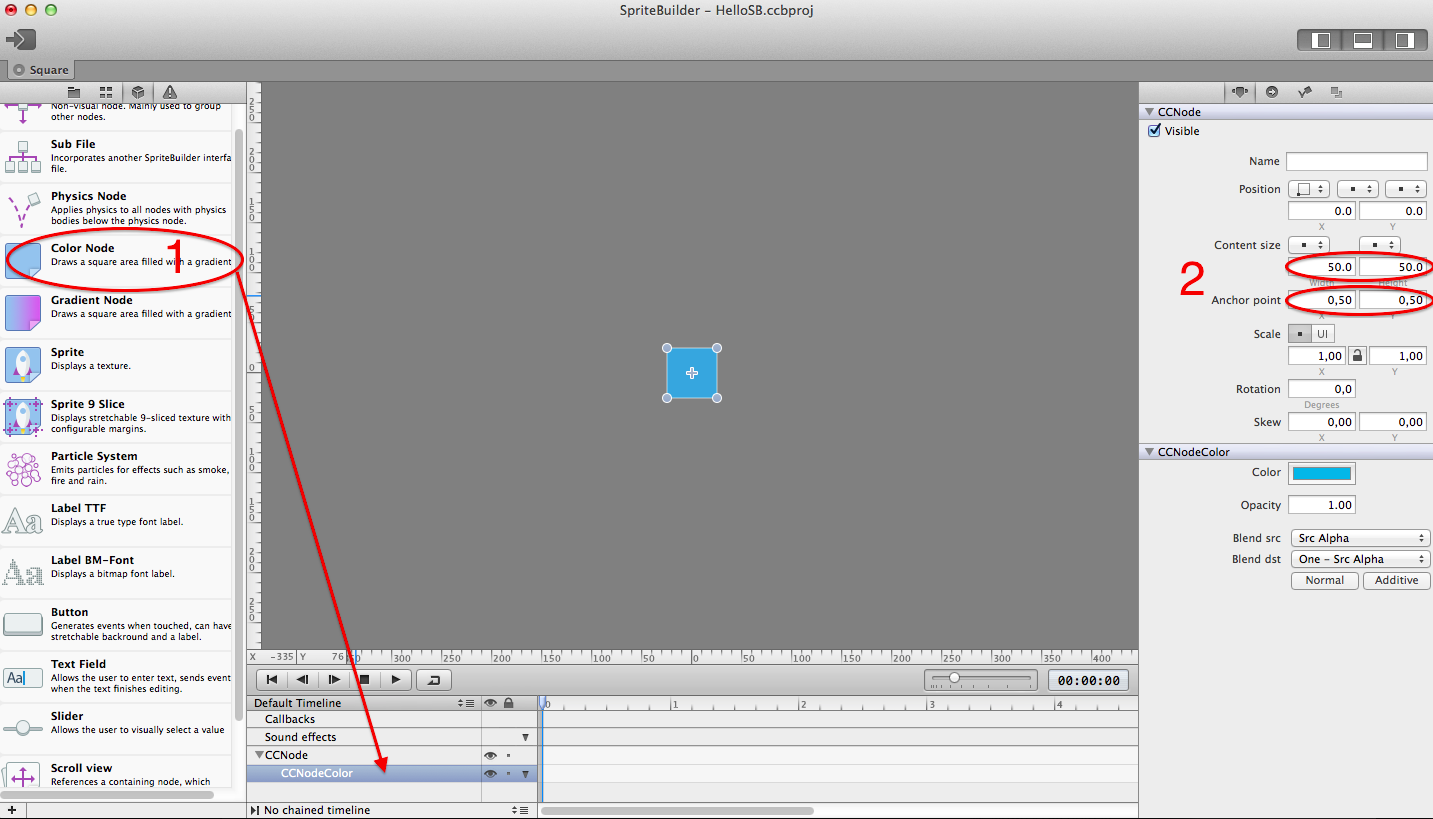
\includegraphics[width=0.9\linewidth]{images/firstproject/square_add_colornode.png}
		%\label{labelstruct} 
\end{figure}
\begin{description}
\item[(1)] Open the \textit{Node Library} and drag a \textit{Color Node} to the
stage or the timeline in order to add it to the root node of of
\textit{Square.ccb}.
\item[(2)] Center the new \textit{Color Node} on the root node by selecting an
\textit{Anchor Point} of (0.5, 0.5). Change the \textit{Content Size} of the
node to (50, 50).
\end{description}

Now the basic square is set up. Next, we need to set up a code connection. Earlier you have seen
the use of \textit{Custom Classes} and \textit{Callbacks}, now we will use the
third type of code connections supported by \SB{} a \textit{Variable
Assignment}.\index{Code Connections!Variable Assignment}. Variable assignments
are generally used when we want to access a part of our scene graph in code. In
our game, whenever a new square is created we want to set a random color for
this square. Generating a random color is something we need to do in code and
cannot do in \SB{}. This also means that we need a way to \textit{apply} the random color we
generate in code to our square that we have set up in \SB{}. The displayed color
is defined in the \textit{Color Node} that we just added. We will need a
reference to this \textit{Color Node} to change the color of our square from
code. \textbf{Select CCNodeColor from the timeline} (and make sure that you
have selected the Color Node and not the Root Node!) and open the connection tab
(the second tab on the right pane):
\begin{figure}[H]
		\centering
		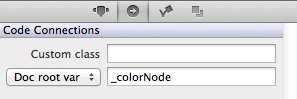
\includegraphics[width=250pt]{images/firstproject/square_code_connection.png}
\end{figure}
As the variable name (entered in the text field), choose \textit{\_colorNode}.
As the second option you need to choose the object to which this variable will be
assigned to. Just as for callbacks you can choose between the \textit{Document
Root} and the \textit{Owner} (\ref{DocumentRoot_Owner}). We choose the
\textit{Document Root}, which means that \SB{} will attempt to store a reference
to the \textit{Color Node} in an instance variable called \textit{\_colorNode}
 on the root node object of this \ccbfile{}. We now face the same 'problem' as earlier when we set up a
\textit{Callback}. The root node of \textit{Square.ccb} is a plain \ccnode{} and
a plain \ccnode{} does not have an instance variable called
\textit{\_colorNode}! We once again need to define a custom class for the root
node of this \ccbfile{}.

\begin{lamp}[frametitle={Variable Assignments, Callbacks and Custom Classes}] 
Always remember that you practically cannot set up a \textit{Variable
assignment} or a \textit{Callback} for the \textit{Document Root} without also
setting a custom class for the root node of the corresponding \ccbfile{}. %TODO:
%flesh out?
\end{lamp}

\textbf{Select the root CCNode node} from the timeline and set the custom class
for this node to \textit{Square}:
\begin{figure}[H]
		\centering
		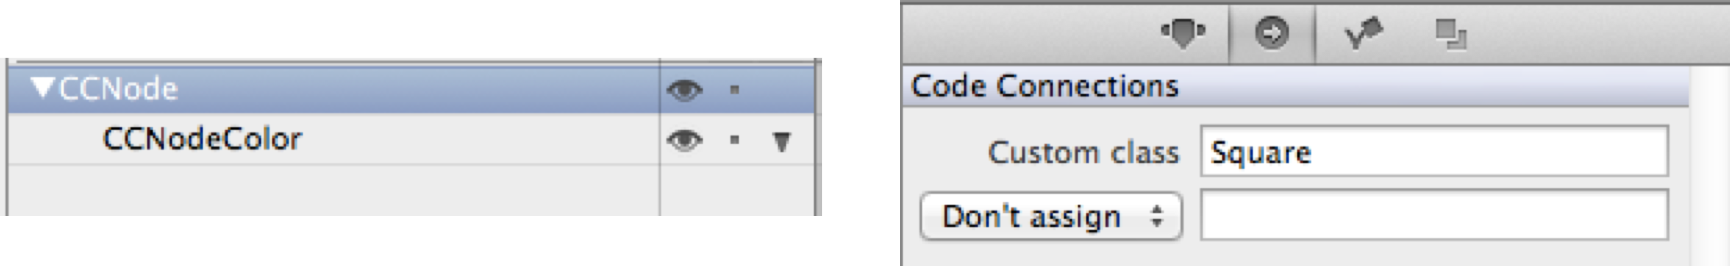
\includegraphics[width=350pt]{images/firstproject/square_custom_class.png}
\end{figure}
When the \textit{CCBReader} reads this \ccbfile{} it will create instance of the
class \textit{Square} as the root node and it will assign a reference to the
\textit{Color Node} to an instance variable of \textit{Square} called
\textit{\_colorNode}. This way we will be able to access the \textit{Color Node}
and change the color of our square programmatically!

\subsubsection{Setting up a custom class for the Gameplay}
In our \textit{Gameplay} scene we want to respond to touches and spawn squares.
All of that functionality needs to be implemented in code. Therefore we need to
define a custom class for the root node of our \textit{Gameplay.ccb} (if you
struggle with the following instructions you can double check how we set up a
custom class for \textit{Square.ccb}).

\begin{enumerate}
  \item Open \textit{Gameplay.ccb}
  \item Select the root \ccnode{} from the timeline
  \item Open the code connections tab (the second tab on the right pane)
  \item Define the \textit{Custom Class} to be \textit{Gameplay}
\end{enumerate}

We've set up multiple code connections throughout this chapter. In order for all
of them to work, we need to \textbf{publish the \SB{} project} and switch to the
\xcode{} project and create the classes and instance variables that we are referencing in the \SB{} project.

\subsubsection{Creating the Square class}
Open \xcode{} and create a new Objective-C class by selecting \textit{File ->
New File\ldots} and choosing \textit{Objective-C class}. As class name choose
\textit{Square} and define it to be a subclass of \ccnode{}. Remember, a custom
class always has to be a subclass of the node type you have selected in \SB{}.
The node type of the root node of \textit{Square.ccb} is a \ccnode{} therefore
\inlinecode{Square} needs to be a subclass of \ccnode{}.

Now open \textit{Square.m} and add the instance variable
\inlinecode{\_colorNode} to the \inlinecode{Square} class. This variable is the
one that we defined in \SB{} to store the reference to the
\inlinecode{CCNodeColor} that displays the color of our square:

\begin{lstlisting}
#import "Square.h"

@implementation Square {
  CCNodeColor *_colorNode;
}

@end
\end{lstlisting} 
After adding the instance variable the code for \textit{Square.m} should look as
shown above. Now that we have a reference to the \inlinecode{CCNodeColor} we
need a position in code where we can set a random color for that node.

The requirements for this projects state that we need to choose a random color
for our Square as soon as it is added to the Gameplay scene. \textbf{How can we
be informed about the square being added to the Gameplay scene?} Therefore we
need to take a closer look at what we call the \textbf{Node
Lifecycle}\index{Node Lifecycle}.

We have five important methods that inform us about certain lifecycle events on
\ccnode{} subclasses. All of the methods below are called on all nodes that are
part of the scene that is being loaded/presented/hidden:

\begin{description}
  \item[didLoadFromCCB] this method is called when the \inlinecode{CCBReader}
  has created the complete node graph from a CCB file and all code connections
  are set up. You implement this method to access and manipulate the content of
  a node. You cannot access child nodes of the node or code connection
  variables before this method is called. Note that this method is only called
  on nodes that are loaded from \ccbfile{}s.
  \item[onEnter/onEnterTransitionDidFinish] are called as soon as a node enters
  the stage. If you are presenting a scene with an animated transition,
  \inlinecode{onEnter} will be called on that scene as soon as the transition
  starts and \inlinecode{onEnterTransitionDidFinish} will be called when the transition
  completes. If a scene or node is being presented/added without an animated
  transition both methods are called directly after each other.
  \item[onExitTransitionDidStart/onExit] are called as soon as a node leaves the
  stage. If you are hiding a scene with an animated transition,
  \inlinecode{onExitTransitionDidStart} will be called on that scene as soon as
  the transition starts and \inlinecode{onExit} will be called when the
  transition completes. If a scene or node is being hidden/removed without an
  animated transition both methods are called directly after each other.
\end{description}

You will get to see lots of examples of how to use the lifecycle methods
throughout this book, for now we know that we need to override
\inlinecode{onEnter} to pick and apply a random color for our square as soon as
it gets added to the Gameplay scene. It is also important to know that you need
to call the \inlinecode{super} implementation if you override any of the 
\inlinecode{onEnter\ldots} or \inlinecode{onExit\ldots} methods. \ccnode{}
has its own implementation of these methods and they are important for the
functionality of the framework - if you do not call them this will result in
unexpected behaviour throughout your game. 
\begin{details}[frametitle={Overriding \cocos{} lifecycle methods}]
As of \cocos{} 3.1 not calling \inlinecode{super} when overriding one of these
lifecycle methods will result in a compiler warning - this can save a lot of
debugging time. You are interested in how that can be done? \cocos{} makes use
of a nice compiler feature to implement this requirement. You simply need to
add an according \inlinecode{\_\_attribute\_\_} to the method definition:

\begin{lstlisting}
 -(void) onEnter __attribute__((objc_requires_super));
\end{lstlisting}

\end{details}
Add this implementation of
\inlinecode{onEnter} to \textit{Square.m}:
\begin{lstlisting}
- (void)onEnter {
  [super onEnter];
  
  // arc4random_uniform(N) generates a random number between 0 and N-1
  float red =   arc4random_uniform(256) / 255.f;
  float green = arc4random_uniform(256) / 255.f;
  float blue =  arc4random_uniform(256) / 255.f;
  
  _colorNode.color = [CCColor colorWithRed:red green:green blue:blue];
}
\end{lstlisting}
The lines above generate three random numbers, one for each color component
with a value between 0.0 and 1.0. These three numbers are used to create an
instance of \inlinecode{CCColor} and set it as the color of our node. 

Now the square will appear in a random color as soon as we add it to a scene.
The second requirement for our square is that it shall rotate while on the
screen. One of the ways to move and/or animate a node in \cocos{} is using the
\cocos{} Action System\index{Action System}. The Action System provides a simple
and expressive way for developers to implement animated changes like:
\textit{Move the main character to the top left corner in 2 seconds}. 

The Action System consists of
dozens of subclasses of \inlinecode{\ccaction{}} - a majority of these actions represent some type of animated movement or
transformation. \inlinecode{CCActionMoveTo} for example moves a node to a
target position within a provided time interval. This is how to use it:
\begin{lstlisting}
CCAction *move = [CCActionMoveTo actionWithDuration:2.f position:ccp(20, 100)];
[aSimpleNode runAction:move];
\end{lstlisting}
All actions can be run by calling the \inlinecode{runAction} method and
providing the action as an argument. 

\begin{details}[frametitle={More about the
\cocos{} Action System}] The \cocos{} Action System is one of the most
important building blocks for most games and we will discuss it in detail
throughout this book. If you want to learn more about the \cocos{} action system
right away, you can check the according chapter in the \cocos{} documentation:
\url{https://www.makegameswith.us/docs/#!/cocos2d/1.0/animations-movements}
\end{details}

The Action System also provides several actions that take other actions as
arguments. One example is \inlinecode{CCActionReverse} that reverses the action
it is initialized with - for example moving a node backwards instead of
forwards. Another example is \inlinecode{CCActionRepeatForever} that takes
another action and - exactly, repeats it forever!

Add the following lines to the \inlinecode{onEnter} method of \textit{Square.m}
to make the square rotate endlessly:
\begin{lstlisting}
CCActionRotateBy *rotate = [CCActionRotateBy actionWithDuration:2.f angle:360.f];
CCActionRepeatForever *repeatRotation = [CCActionRepeatForever actionWithAction:rotate];
[self runAction:repeatRotation];
\end{lstlisting}
One of the nicest aspects of the Action System is that it produces very readable
code, just as the one shown above. We rotate our square by 360 degrees in 2
seconds and repeat that forever!

Finally our implementation of \inlinecode{Square} is complete. Along the way you
have learned about code connections, generating random numbers and using the
action system. Now let's move on to implement the \inlinecode{Gameplay} class so
that we can see our delightfully colored and rotating squares in action.

\subsubsection{Creating the Gameplay class}

After we have set up all the code for the square it's now time to implement the
gameplay. In \SB{} we have already created the \ccbfile{} \textit{Gameplay.ccb}
and set up the custom class for the root node to be \inlinecode{Gameplay}. Now we need to add the
\inlinecode{Gameplay} class in \xcode{} and implement touch handling code that
creates a square and adds it to the gameplay scene as soon as a player touches
the screen.

Create the new class just as you have created the \inlinecode{Square} class. In
\xcode{} select \textit{File -> New -> File\ldots} and select
\textit{Objective-C} class. Again, this class needs to be a subclass of
\ccnode{} since the root node of \textit{Gameplay.ccb} is a \ccnode{}.

\subsubsection{Adding Touch Handling to the Gameplay}
Now we need to add touch handling to the Gameplay scene. This will be the first
time you will add User Interaction to a \cocos{} game! 

The \cocos{} touch handling system works on a \textit{per node
basis}\index{Touch Handling}.
This means that every \ccnode{} instance can choose to receive touches or not. You
can activate touch handling on any node using the
\inlinecode{userInteractionEnabled} property. If
\inlinecode{userInteractionEnabled} is set to \inlinecode{YES}, \cocos{} will
automatically check if your node is touched by the user. In \cocos{} the front
most node receives touch events first.

Each touch in \cocos{} has a lifecycle. That lifecycle consists of four
different states and four corresponding methods that are called on your
\ccnode{}:

\begin{description}
\item[touchBegan:] called when a touch begins
\item[touchMoved:] called when the touch position of a touch changes
\item[touchEnded:] called when a touch ends because the user stops touching the
screen
\item[touchCancelled:] called when a touch is cancelled because user moves touch
outside of the touch area of a node
\end{description}

You can override all of these methods in any \ccnode{} subclass in order to
respond to these lifecycle events. For our simple example now, we only need to
respond to the \inlinecode{touchBegan:} method.

\begin{details}[frametitle={The \cocos{} Touch System}]
We will see more complicated use cases of the \cocos{} touch system throughout
other examples in this book. If you are interested in more details right away
you should
read:\url{https://www.makegameswith.us/docs/#!/cocos2d/1.1/user-interaction} and
\url{https://www.makegameswith.us/gamernews/366/touch-handling-in-cocos2d-30}.
\end{details}

Now that you know the basics, let's implement touch handling for the
\inlinecode{Gameplay} class. First, we need to enable user interaction. A great
place to do this is in the \inlinecode{onEnterTransitionDidFinish} method. Why?
If you have an animated transition that presents your gameplay scene you will
likely not want to the player to interact with your game before this transition
has finished entirely. Add the following method to \textit{Gameplay.m}:
\begin{lstlisting}
- (void)onEnterTransitionDidFinish {
    [super onEnterTransitionDidFinish];
    
    self.userInteractionEnabled = YES;
}
\end{lstlisting}
As discussed earlier you need to call the \inlinecode{super} implementation of
the lifecycle method you are overriding. In the second step we are setting
\inlinecode{userInteractionEnabled} to \inlinecode{YES}. Now \cocos{} knows that
this node wants to receive touch events. 

In the next step we need to decide to which touch events we
want to subscribe and implement the corresponding method. For this simple game
we only need to know when a touch begins, because we will add a square to the
screen immediately. This means we only need to implement the
\inlinecode{touchBegan:} method. Add the following implementation to
\inlinecode{Gameplay.m}:
\begin{lstlisting}
- (void)touchBegan:(UITouch *)touch withEvent:(UIEvent *)event {
    CGPoint touchPosition = [touch locationInNode:self];
    CCNode *square = [CCBReader load:@"Square"];
    [self addChild:square];
    square.position = touchPosition;
}
\end{lstlisting}
We have now implemented the \inlinecode{touchBegan:} method. It will be called
every time the user taps onto the gameplay scene. As one parameter of this
method we receive a \inlinecode{UITouch}. The \inlinecode{UITouch} stores all
information about the touch. \cocos{} adds a method called
\inlinecode{locationInNode:}. This method returns the touch position
relative to the provided node. In the first line we call this method to receive
the touch location within the gameplay scene (referred to by \inlinecode{self}).
In the next line we load one \inlinecode{Square} node using the
\inlinecode{CCBReader}. Then we add that loaded square as a child to the
gameplay scene. The \inlinecode{addChild:} method of \ccnode{} will add the
square to the node hierarchy of the gameplay scene. As soon as node becomes part
of the node hierarchy of the currently active scene it will be displayed on the
screen. Finally we choose a position for the square.
We provide the touch position that we determined in the first line - this way the square will be spawned exactly at the position touched by
the player. Now it's time to run your project again. Once the game started,
select the \textit{Start} button to go to the gameplay scene then click onto the
screen multiple times to simulate touches. Every time you simulate a touch you
should see a new square spawn at the touch position:
\begin{figure}[H]
		\centering
		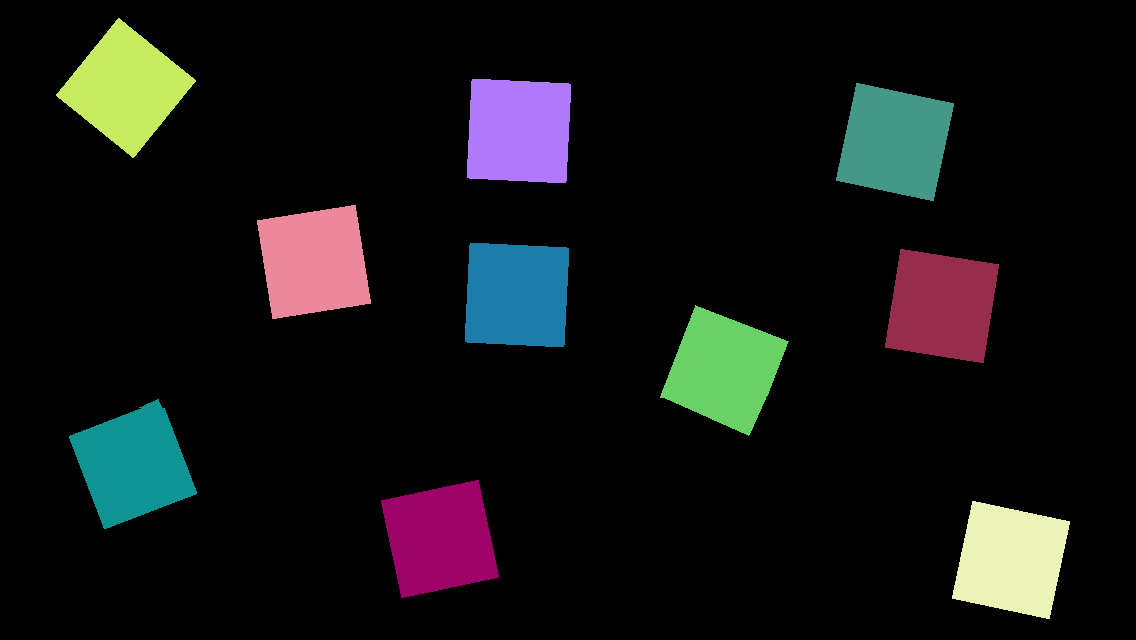
\includegraphics[width=350pt]{images/firstproject/spinning_squares.png}
\end{figure}
\textbf{Well done!} You have come a very long way from the blank project to a
first simple game that uses scene transitions, actions and the \cocos{} touch
system. But this is only the very beginning. In the next chapter we will start
working on a much more complex game that will teach you many more important
concepts of \SB{} and \cocos{}. 

\chapter{A Game with Assets in SpriteBuilder}

Graphics and Sounds are the essence of every good game. In the first chapter
you have learned the very basics of \SB{} and \cocos{} by building a game that only
uses plain colored shapes. In this chapter you will learn how \SB{} helps you to
integrate assets into your game. Learning by example is the most fun, so we will
build a small game throughout this chapter that uses all aspects of asset
management.

\section{Adding Assets to a SpriteBuilder project}
Start by creating a new \SB{} project for this game. I have called the
project \textit{FallingObjects}.

Now you should download the assets from
\url{https://dl.dropboxusercontent.com/u/13528538/SpriteBuilderBook/assets.zip}.
Once the download completes you add the assets to the project by dragging the
entire folder into the left \textit{File View} in the left panel of
\SB{}:\index{Assets!Adding Assets}

\begin{figure}[H]
		\centering
		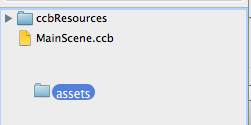
\includegraphics[width=200pt]{images/Chapter2/DragAssets.png}
\end{figure}

Great, now we have some assets to use in our game. Now is a good time to take a
close look at how \SB{} and \cocos{} handle assets.

\section{Asset Handling in \SB{} and \cocos{}}
One of the main goals of \SB{} is to make game development for multiple device
types as easy as possible. This means that games should automatically be able to
run on differently sized iPhones, iPads and Android Devices. Since each of these
devices has a different resolution \cocos{} and \SB{} allow developers to use different assets to target them. \SB{}
provides four different resolution categories:
\begin{description}
\item[phone] resolution for non-retina iPhone and Android devices
\item[phone-hd] retina resolution for iPhone and Android
\item[tablet] resolution for non-retina iPad and Android tablets
\item[tablet-hd] resolution for retina iPad and Android tablets
\end{description}

Luckily using \SB{}, there is no need to provide four resolutions for each asset
thanks to \textbf{automatic downscaling}\index{Assets!Automatic Downscaling}.
Per default \SB{} assumes that all assets added to a project are provided in \textit{tablet-hd} resolution, then
\SB{} generates downscaled images for the other resolutions. While you can
provide different images for four targets, \SB{} only knows three resolution
types:
\begin{description}
\item[1x] non-retina images
\item[2x] retina images
\item[4x] double sized retina images
\end{description}

By default \SB{} maps these resolution types to the different devices in a way
that every asset has the same size (in relation to the screen size) on every
device. This means games running on an iPad will look very similar to games
running on an iPhone, except that the have a slightly different aspect ratio.
Here is an example from on of our tutorials showing what a game looks like on
different device types:

\begin{figure}[H]
		\centering
		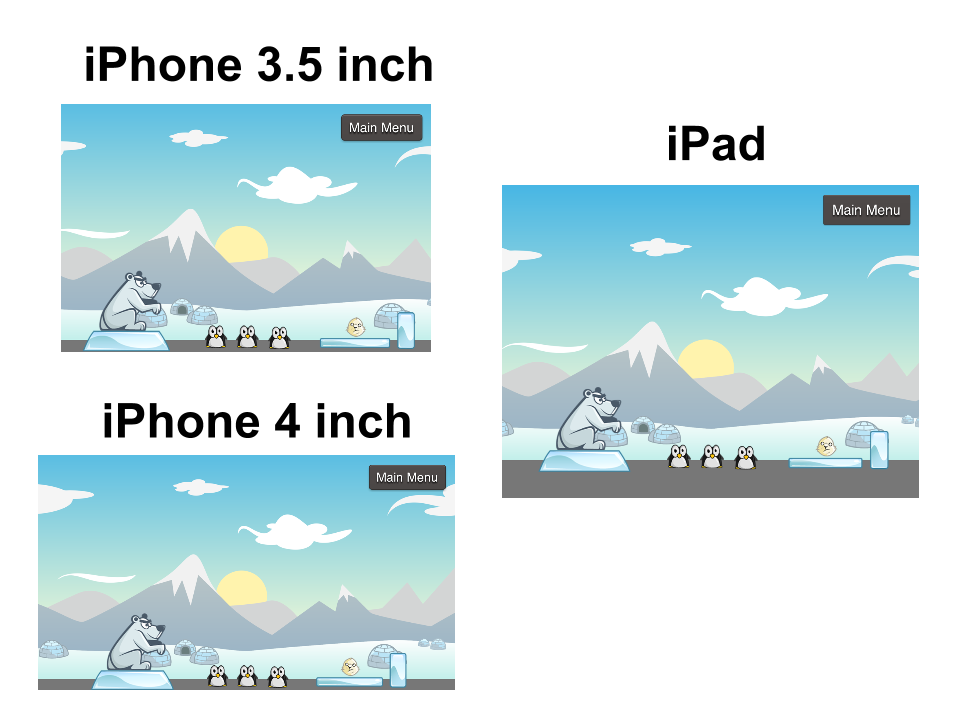
\includegraphics[width=0.9\linewidth]{images/Chapter2/ResultsFlexibleScaleMode.png}
		\caption{From our tutorial \textit{Dynamic Layouts with SpriteBuilder and
		Cocos2D}}
\end{figure}

Let's take a look at where all the settings I mentioned are visible in the \SB{}
UI. When you open the project settings (\textit{File -> Project Settings\ldots})
you can see the available downscaling options:

\begin{figure}[H]
		\centering
		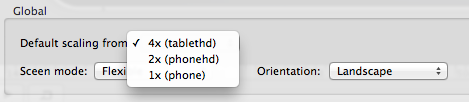
\includegraphics[width=300pt]{images/Chapter2/DownScalingGlobal.png}
\end{figure}

This setting defines the \textit{global} downscaling option. Individual assets
can define their own behaviour, thereby overriding this global setting. To make
support of multiple devices as easy as possible you should provide all of your
assets in \textit{4x} resolution and keep this default setting.

When you select an individual asset from the File View you can see different
downscaling settings:

\begin{figure}[H]
		\centering
		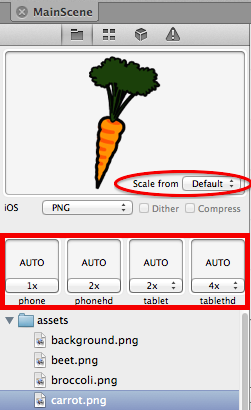
\includegraphics[height=200pt]{images/Chapter2/DownScalingPerAsset.png}
\end{figure}

Each asset can have its own \textit{Scale from} setting. \textit{Default} means
that the global project setting applies (in this project: downscaling from
\textit{4x}). Additionally you can see how the different resolution types are
mapped to the different device types. Here you could for example choose that a
certain asset should not be scaled up on retina tablets by choosing a
\textit{2x} resolution for \textit{tablethd} - however, the default settings
work best most of the time.

For future reference, this is an example that shows you which sizes your assets
will have on the different devices by default:

\begin{table}[H]
\begin{tabular}{llll}
\textbf{Device} & \textbf{Default Resolution Type} & \textbf{Size on Screen (points)} & \textbf{Size in Pixels} \\
iPhone          & 1x                               & 50x50                            & 50x50                   \\
iPhone Retina   & 2x                               & 50x50                            & 100x100                 \\
iPad            & 2x                               & 100x100                          & 100x100                 \\
iPad Retina     & 4x                               & 100x100                          & 200x200                
\end{tabular}
\end{table}

You can see, if you have a size in mind for a certain asset on an iPhone you
should provide the asset in four times larger resolution.

A last interesting case are background images that you want to work for
all 4 resolutions. A solution is discussed in
the Q\&A section (\ref{background_all_resolutions}).

\begin{details}[frametitle={Different images for different devices}] 
You can not only change the scaling option for an asset on different devices,
you can even use an entirely different image for a certain resolution. You can
do that by dragging an image \textbf{that is currently not part of the \SB{}
project} from Finder into one of the four boxes below the asset preview:
%TODO: note this fact in docs as well
%TODO: ask viktor why this displays the image for tablet and not for phone in SB
\begin{figure}[H]
		\centering
		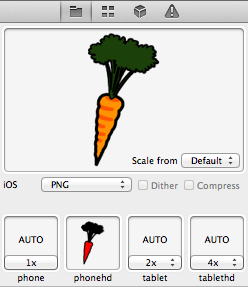
\includegraphics[height=140pt]{images/Chapter2/DifferentImageDevice.png}
\end{figure}

Note that images you add this way will be displayed in exactly the size you have
added them and will not be downscaled.

\end{details}

\begin{details}[frametitle={Behind the scenes}] 
If you are interested in how \SB{} and \cocos{} organize assets you can take a
look at the resource package
(\textit{/Packages/\allowbreak{}SpriteBuilder Resources\allowbreak{}.sbpack}) by
right-clicking and selecting \textit{Show Package Contents}:
\begin{figure}[H]
		\centering
		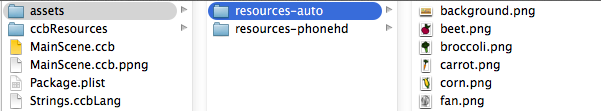
\includegraphics[width=280pt]{images/Chapter2/behindscenes_resourcepack.png}
\end{figure}
You will see that \SB{} groups images inside the assets folder into a
\textit{resources-auto} folder, all images in that folder are subject to
automatic downscaling. If you explicitly add images for a certain resolution as
shown with the carrot in the above example, a new folder for that resolution
(e.g. \textit{resources-phonehd}) is created.

In \cocos{} a class called \inlinecode{CCFileUtils} is responsible for loading
the correct images for the current device during runtime. \SB{} uses a special
configuration of \inlinecode{CCFileUtils} that is set up in
\inlinecode{[CCBReader configureCCFileUtils]}. \index{Framework
Classes!CCFileUtils}
\end{details}

\section{Adding the background image}
Now that we have a basic understanding of how asset management works, lets get
started working on our game. For now our game will only consist of one scene, so
we can start working in the \textit{MainScene.ccb} that is part of the \SB{}
template. First, remove the existing content so that we can start with a blank
scene. Now we can add the background image. To add a sprite to a scene we can
simply drag the asset to the stage, \SB{} will automatically create an instance
of \ccsprite{}. Add the \textit{background.png} image to the stage.

How should we position this background image? We already have briefly discussed
the \SB{} positioning system (\ref{PositioningSystem}). Using the positioning
system correctly is especially important when we create games for phones and tablets -
which we always should try to do. In most cases - like in this game it is the
best to center the background image. That way phones and tablets will display a
very similar portion of the background image. You can center the image by
choosing a \textit{normalized} position type (\textit{in \% of parent
container}) and setting the position to (50, 50).

\begin{figure}[H]
		\centering
		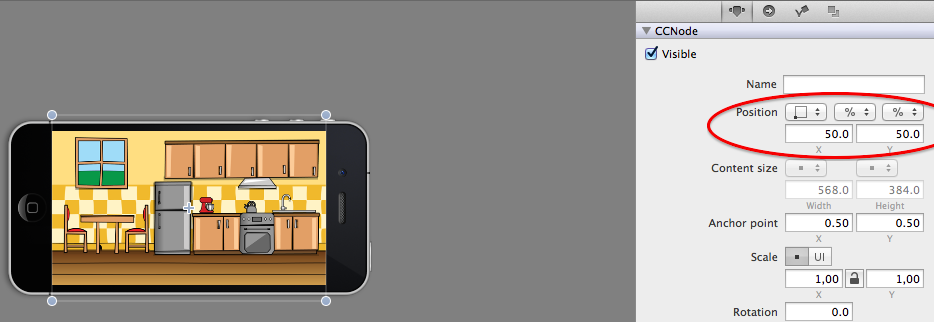
\includegraphics[width=0.9\linewidth]{images/Chapter2/center_background.png}
\end{figure}

You can preview what your game will look like on different device types directly
in \SB{}, without the need to compile and run the game - you should do this as
often as possible! The option is available from the menu \textit{Document ->
Resolution}. You can also use the CMD+1, CMD+2 and CMD+3 shortcuts. This feature
will allow you to preview the game on a 3.5-inch iPhone, a 4-inch iPhone and an
iPad.

\section{Create falling objects}
Now let's dive into the implementation of the actual game. The next step should
be adding falling objects. Our game will have two categories of objects, ones
that should be caught (food) and ones that shouldn't (electronic devices).

In total we have over ten different objects in our game but these just exist as
visual enhancement, actually we are only differing between two types of objects.
One way to implement the falling objects would be creating a \ccbfile{} for each
object but that isn't actually necessary for this game. We need to create all
falling objects dynamically, while the game is running, and for each object we
only need to store if it should be caught or not. That can be best accomplished
by a subclass of \ccsprite{} that we create in code. This way you will also
learn how to use assets you added in \SB{} to create \ccsprite{}s in code.
Open the \xcode{} project of the game to get started.

\subsection{Create a falling object class}
In general we have two ways to differentiate objects a player should catch and
ones he shouldn't catch. We could:
\begin{itemize}
  \item Create two distinct subclasses of \ccsprite{}, each representing one
  type of object
  \item Only have one subclass and add a \inlinecode{type} property to it
\end{itemize}
Since our falling objects won't have any type-specific behaviour, creating two
distinct subclasses is not necessary in this case. Instead, as of now, one
subclass with a \inlinecode{type} property is the better solution.

Create a new class called \inlinecode{FallingObject} and make it a subclass
of \ccsprite{}. The best way to represent different types in Swift is
using enumerations. Add this enum definition to \textit{FallingObject.swift},
inside of the \inlinecode{class} block:

\begin{lstlisting}
enum FallingObjectType: Int {
  case Good
  case Bad
}
\end{lstlisting}

Swift supports multiple types of enumerations and enumeration values.
In the example above we are creating an enumeration with \textit{Raw Values}.
When we use an enumeration with raw values we need to assign a type as part of
the enum definition, as shown in the first line (\inlinecode{enum
FallingObjectType: Int}). Each enum value will be mapped to one value of this
provided type. In the example shown above, the raw value for
\inlinecode{FallingObjectType.Good} will be 0 and the value for
\inlinecode{FallingObjectType.Bad} will be 1. Thanks to auto-increment we do not
need to map entries to numbers explicitly. Associating enum values with raw values is optional,
throughout this chapter you will see why this feature is useful to us.

\begin{details}[frametitle={Enumerations in Swift}] 
You can read everything about the different ways of creating enumerations in
Swift in the official documentation
(\url{https://developer.apple.com/library/ios/documentation/
Swift/Conceptual/Swift_Programming_Language/Enumerations.html}).
\end{details}

Additionally we add an instance variable to store the object type. Later we will
add an initializer to set the type of the falling object. For now your class
should look as follows:

\begin{lstlisting}
import Foundation

class FallingObject: CCSprite {

  enum FallingObjectType: Int {
	case Good
	case Bad
  }
    
  private(set) var type:FallingObjectType
  
}
\end{lstlisting}

We define the instance variable to be \textit{readonly} because we will not
support changing the type of a falling object after it has been created. In Swift we can 
define variables as \textit{readonly} by marking the \textit{setter} as private.

Note that the code will not compile at this point. Since \inlinecode{type} isn't
declared as an optional value, Swift requires us to provide an initializer that
sets this value. We will fix this in the next chapter.

\subsection{Choose an asset for a falling object}
We want the game to spawn entirely random falling objects. As you remember we
have a couple of assets for both types of objects. Whenever we spawn an object
we will need to choose a random asset, based on the object type. A good place to
implement this functionality is directly in the \inlinecode{FallingObject}
class. We can provide a custom initializer that allows the class to be initalized with an object type.
When this initializer gets called we choose a random asset and apply it as a
texture to the \inlinecode{FallingObject}.

How can we create a list of images for objects that should be caught (e.g.
food) and ones that shouldn't (e.g. radios)? One way of implementing this would
be creating two arrays, one for each object type, and storing filenames for 
different assets in these arrays. As good game developers however, we try to
keep game content and code as separated as possible. That makes it easier to
update the list of assets later on and it keeps our codebase small and well
structured. So instead of creating these arrays in code we could use some sort
of resources file that stores information on available images. A very common 
format for storing such type of information in Cocoa Touch is a \textit{plist} 
(Property List). You can create a \textit{plist} by selecting \textit{File ->
New -> File\ldots} from \xcode{}'s menu. 
Then you need to select \textit{Resource} from the left panel and choose
\textit{Property List} on the right:

\begin{figure}[H]
		\centering
		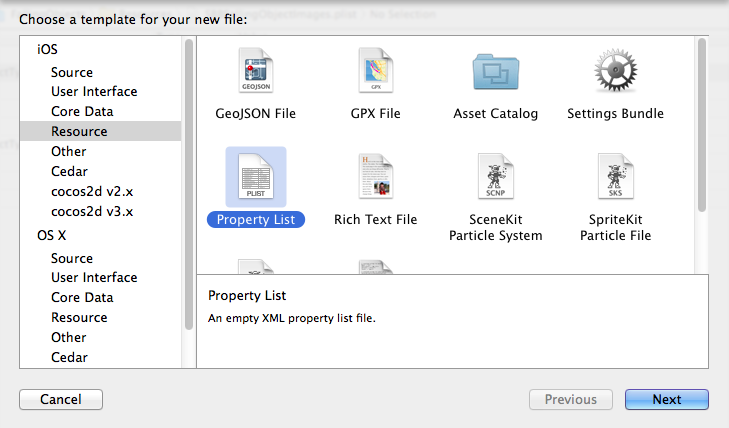
\includegraphics[width=300pt]{images/Chapter2/create_plist.png}
\end{figure}

As the name choose \textit{FallingObjectImages}. Now fill the \textit{plist}
with two arrays that contain the filenames of the assets that we added in \SB{}.
When accessing assets from a \SB{} project you always need to include folder
names. Instead of referencing the tomato with \inlinecode{tomato.png} you need
to use \inlinecode{assets/tomato.png} since the asset is in the
\inlinecode{assets} folder in the \SB{} project:

\begin{figure}[H]
		\centering
		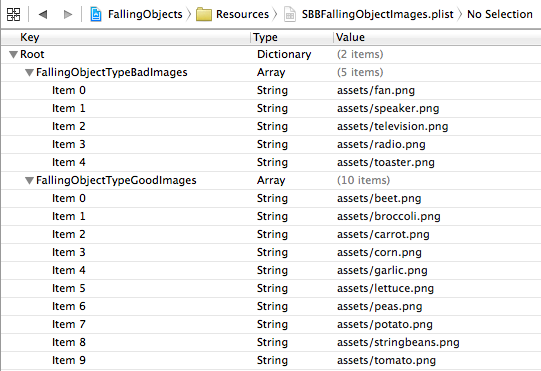
\includegraphics[width=0.7\linewidth]{images/Chapter2/plist_setup.png}
\end{figure}
Now we have a list of all asset names grouped into the two object type
categories. Time to implement the \inlinecode{FallingObject} class.

When a falling object is initialized we want to
choose random image from the \textit{plist} that we just created.
The first step is loading the \textit{plist} in code. Luckily \textit{plists}
consist of Dictionaries, Arrays, Strings, etc. and all of these types exist in
Swift as well - there are some very convenient methods to load
\textit{plists}. 

During each playing session we are going to create hundreds of
falling objects. Since the images that represent these objects won't change it
would be a waste of resources to load the \textit{plist} every time we create a
new instance of \inlinecode{FallingObject}. Instead we should only load it
once and then keep a reference to it for future use. A good way of doing this is
using a class constant to store the \textit{plist} reference once it is loaded.

\begin{details}[frametitle={Class variables in Swift}] 
While class constants and non-computed class variables are already specified as
part of the Swift language they aren't implemented in the Swift compiler yet 
(as of Xcode version 6.1.1), therefore we need to use a workaround. 
\end{details}

As described in the detail box above, Swift does not yet support class
constants, therefore we need to use a workaround. Here is the code that loads
the plist and stores the content in a class variable. You should place it within
the class definition of \inlinecode{FallingObject} (no worries, we will discuss
the code in detail right away):

\begin{lstlisting}
  private class var imageNames:ImageNames {
    struct ClassConstantWrapper {
      static let instance = ImageNames()
    }
    return ClassConstantWrapper.instance
  }
  
  private struct ImageNames {
    var good: [String]
    var bad: [String]
    
    init () {
      let path = NSBundle.mainBundle().pathForResource("FallingObjectImages", ofType: "plist")!
      let imageDictionary:Dictionary = NSDictionary(contentsOfFile: path)!
      good = imageDictionary["FallingObjectTypeGoodImages"] as [String]
      bad = imageDictionary["FallingObjectTypeBadImages"] as [String]
    }
  }
\end{lstlisting}

First, we are defining a private class variable. Currently Swift only supports
computed class variables, that means we need to provide a getter that will
return a generated value and does not rely on a class storage variable. We
provide that getter through the closure that is placed directly after the 
variable declaration. Whenever the class variable is accessed
this closure is called. Inside of this closure we place the workaround mentioned
earlier. We declare a struct called \inlinecode{ClassConstantWrapper} with a
static constant called \inlinecode{instance}. This static constant is initialized with an instance of
the structure \inlinecode{ImageNames} which we declare a few lines later. Since
\inlinecode{instance} is a static constant, the expression will only be
evaluated once and only one instance of \inlinecode{ImageNames} will ever be
created, independently of how often the class variable is accessed.

Inside of the \inlinecode{ImageNames} struct, the actual work happens. First we
declare two array variables that store strings. They store the filenames of the
\textit{good} object assets and the \textit{bad} object assets. Inside of the
initializer we fill these variables.

The initializer takes no parameters. The first line gets the path of the
\textit{FallingObjectImages.plist} file. Then we use a convenience initializer
on \inlinecode{NSDictionary} called \inlinecode{contentsOfFile:}. That
initializer creates a dictionary from a provided plist. This only works because
the root element of our plist is a dictionary! 
Earlier we've set up our plist to contain two arrays of strings,
\textit{FallingObjectTypeGoodImages} and \textit{FallingObjectTypeBadImages}
below the root element.
We can now extract these two arrays from our dictionary and assign them to the 
\inlinecode{good} variable and \inlinecode{bad} variable, respectively. During
this assignment we need to cast the arrays into \inlinecode{[String]} arrays
using the \inlinecode{as} operator. This is necessary because we are receiving
an Objective-C Array (\inlinecode{NSArray}) that cannot store type information
about the elements it contains. We however know that this array only contains
strings so we want to treat it as a \inlinecode{[String]} array in Swift.

Due to the necessary workaround this is quite a bit of code, but things will
improve as Swift matures. 

Now we have successfully set up a class constant that will load the required
image names when it is accessed the fist time and store these images on a class
level. That will avoid reloading the plist for every instance of
\inlinecode{FallingObject} that we create.
  
Now that we have access to the image names we can implement the actual
initializer of \inlinecode{FallingObject}. We need to:
\begin{itemize}
  \item Pick a random image based on the object type
  \item Call the designated initializer of our superclass \ccsprite{}
\end{itemize}

This is what the initializer should look like:
\begin{lstlisting}
  init(type: FallingObjectType) {
    self.type = type
    
    var imageName:String? = nil
    
    if (type == .Good) {
      let randomIndex = randomInteger(FallingObject.imageNames.good.count)
      imageName = FallingObject.imageNames.good[randomIndex]
    } else if (type == .Bad) {
      let randomIndex = randomInteger(FallingObject.imageNames.bad.count)
      imageName = FallingObject.imageNames.bad[randomIndex]
    }
    
    let spriteFrame = CCSpriteFrame.frameWithImageNamed(imageName) as CCSpriteFrame
    super.init(texture: spriteFrame.texture, rect: spriteFrame.rect, rotated: false)
    
    anchorPoint = ccp(0,0)
  }
\end{lstlisting}
We start of by storing the type we receive in an instance variable.
Then we create a local variable called \inlinecode{imageName} that we will use
to load the correct texture for this object type. Next, we check whether we are
initializing a good or a bad object. In each case we generate a random number,
using our helper function \inlinecode{randomInteger}, that picks one image name
from the set of available image names in the arrays. %TODO: mention how to add
% helper functions
Next, we need to call an initializer of our superclass \ccsprite{}. Here we run
into another limitation of the current version of Swift: we can only call
\textit{designated} initializers of our superclass, but not any
\textit{convenience} initializers. This means instead of calling:
\begin{lstlisting}
CCSprite(imageNamed: String!)
\end{lstlisting}
We have to call the designated initializer:
\begin{lstlisting}
CCSprite(texture: CCTexture!, rect: CGRect, rotated: Bool)
\end{lstlisting}
This unfortunately means some extra code! We create a \inlinecode{CCSpriteFrame}
with the image name that we have selected from one of our lists, then we use
that sprite frame to call \ccsprite{}'s designated initializer. Finally, we set
the anchor point of our object to the bottom left corner, that will make it
easier to determine the spawn position later on.

That's all we need in order to create a \inlinecode{FallingObject}! Now we
can move on and spawn some objects.

\section{Spawn falling objects}
Now it's time to implement one of the core mechanics of the game: Spawning
objects and make them fall from the top of the screen to the bottom. We are
going to implement this in \textit{MainScene.swift}. 

We will spawn objects after a certain time period. The spawning objects will
start at the top of the screen and fall to the bottom. To not use an
increasing amount of memory we will need to take care of removing objects that
have fallen below the bottom edge of the screen. A good way to do this is
creating an array to store all the objects we spawn. Swift lets us define a
private instance variable and initialize the array stored in it in a single line
of code:

\begin{lstlisting}
class MainScene: CCNode {

  private var fallingObjects = [FallingObject]()

}
\end{lstlisting}

We also need to define a falling speed and an interval at which we want to spawn
objects. A good way to do this is by defining constants - we want to avoid to
have these numbers all over our code. Add the two constants so that your class
definition looks as following:

\begin{lstlisting}
class MainScene: CCNode {

  private var fallingObjects = [FallingObject]()

  private let fallingSpeed = 100.0
  private let spawnFrequency = 0.5
}
\end{lstlisting}

We are going to spawn falling objects with the frequency that we have defined in
the constant \inlinecode{spawnFrequency}. Through the \inlinecode{CCNode} class
\cocos{} provides convenient methods for scheduling repeating events without the
need to instantiate a timer. We schedule that timer in the
\inlinecode{onEnterTransitionDidFinish} method:

\begin{lstlisting}
  override func onEnterTransitionDidFinish() {
    super.onEnterTransitionDidFinish()
    
    // spawn objects with defined frequency
    schedule("spawnObject", interval: spawnFrequency)
  }
\end{lstlisting}

Remember, \textit{onEnterTransitionDidFinish} is called as soon as the
presentation transition is completed and the current scene is fully visible.
This is when we want to kick of the spawning mechanism. 
All we need to provide is a \textit{selector}, which simply means a method name
as a string, and a frequency at which it shall be called. Now, as soon as the
\inlinecode{MainScene} is presented on the stage, the \inlinecode{spawnObject}
method will be called twice a second.
To complete the spawning functionality we will have to implement the
\inlinecode{spawnObject} method and additionally move the spawned objects from
the top of the screen to the bottom.

We want to randomly spawn either positive objects that should be caught or
negative ones that should not, for that we will generate a random number. Based
on the random number we will generate a falling object. We will place that
spawning object just above the screen at a random X position. Here is how we can
implement that:

\begin{lstlisting}
  func spawnObject() {
    let randomNumber = randomInteger(2)
    
    let fallingObjectType = FallingObject.FallingObjectType(rawValue:randomNumber)!
    let fallingObject = FallingObject(type:fallingObjectType)
    
    // add all spawning objects to an array
    fallingObjects.append(fallingObject)
    
    // spawn all objects at top of screen and at a random x position within scene bounds
    let xSpawnRange = Int(contentSizeInPoints.width - CGRectGetMaxX(fallingObject.boundingBox()))
    let spawnPosition = ccp(CGFloat(randomInteger(xSpawnRange)), contentSizeInPoints.height)
    fallingObject.position = spawnPosition
    
    addChild(fallingObject)
  }
\end{lstlisting}

As you can see here, defining the \inlinecode{FallingObjectType} enumeration
with a raw integer value allows us to create a type directly from a number.
Here that comes very handy. Besides that the spawning code is not too exciting,
it primarily consists of a little math and type conversions.

This is a schematic diagram of where we are spawning
objects with the code shown above:

\begin{figure}[H]
		\centering
		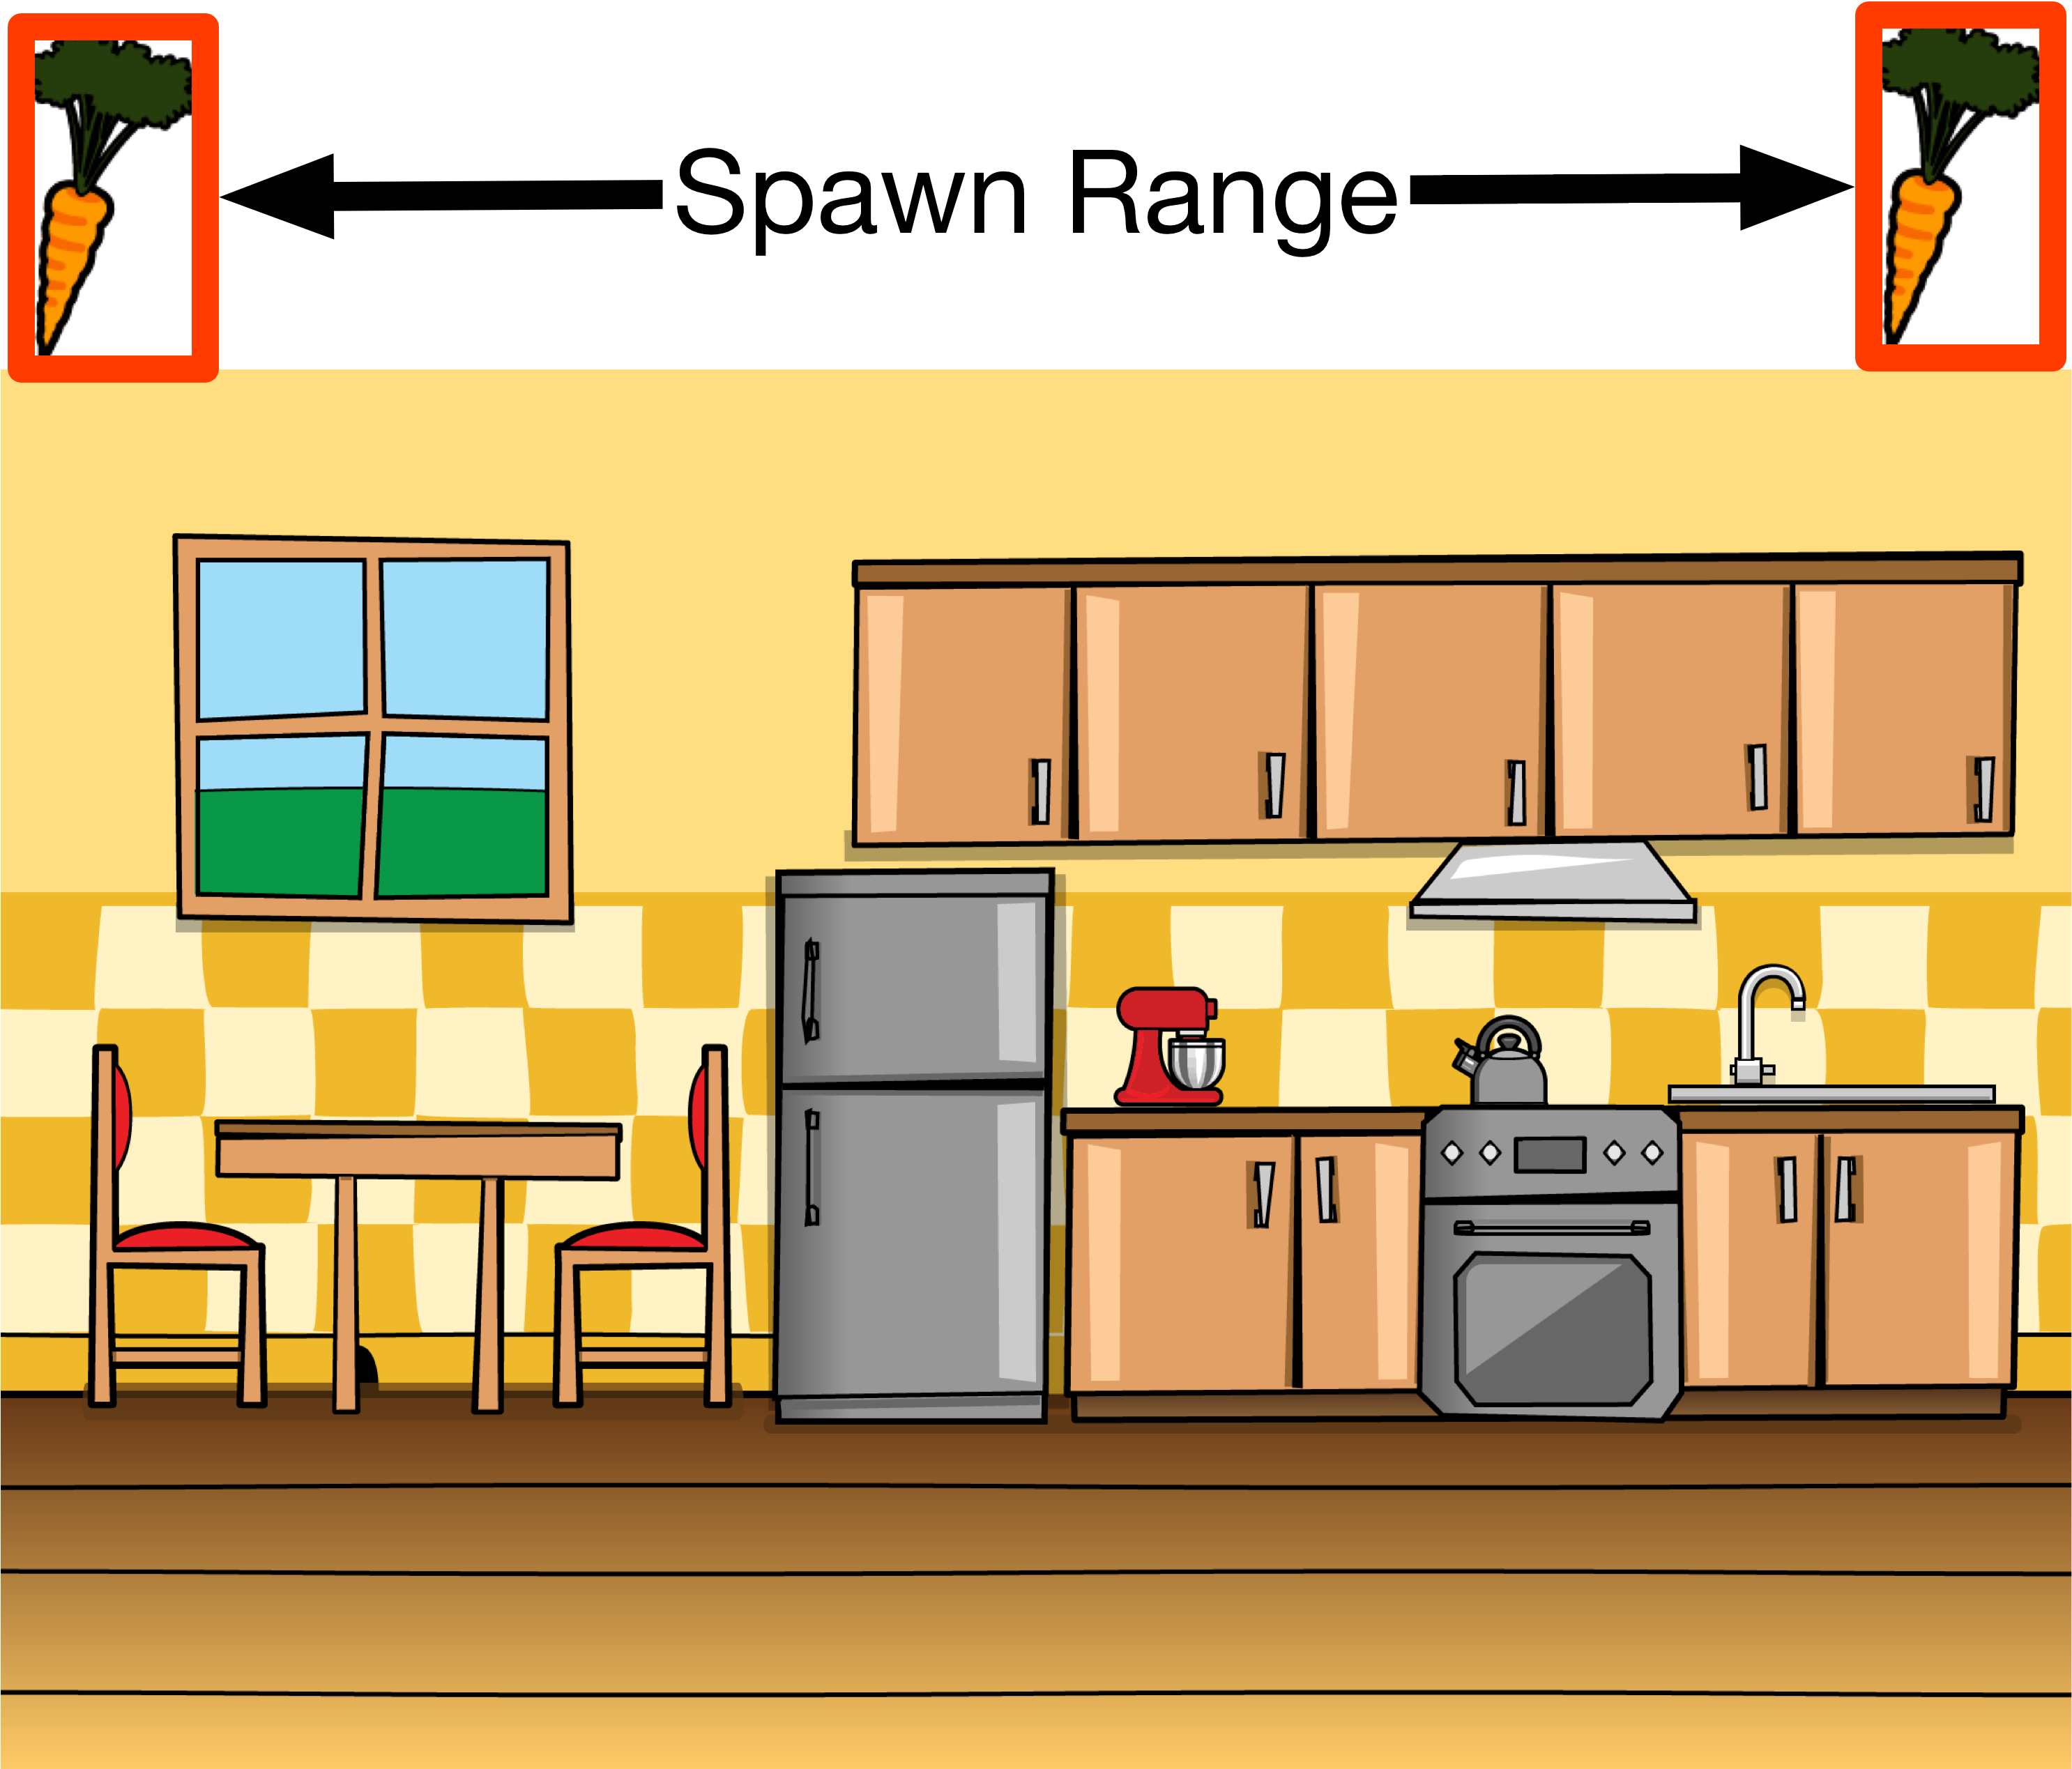
\includegraphics[width=200pt]{images/Chapter2/SpawnObjects.png}
\end{figure}

Our current version of the game spawns new objects twice a second at the top of
the screen and at a random X position. However, these objects don't move yet so
you won't be able to see them falling down. Let's implement the falling code to
complete the entire spawning functionality!

\section{Move falling objects}
The last step for this chapter will be moving the objects we are spawning to the
bottom of the screen. While building your very first \SB{} game you have learned
to use the \cocos{} action system to move nodes. The action system lets us
describe changes over time, e.g. \textit{move 100 points to the right over 2
seconds}. Another option to move nodes that we haven't
discussed yet is using the \cocos{} \textit{update loop}\index{Update Loop}.

\subsection{Update Loop}
When we build games with \cocos{} the engine attempts to render 60 frames a
second and draws theses rendered frames to the screen of the device. When we
move objects between rendering frames, they will appear as moving objects to the
user. \cocos{} provides a method that is called directly before a frame is
rendered, the \inlinecode{update} method.

The \inlinecode{update} method is defined as part of the
\inlinecode{CCSchedulerTarget}\index{Framework Classes|CCSchedulerTarget}
protocol. \inlinecode{CCNode} implements this protocol, that means any subclass
of \inlinecode{CCNode} can override the method. This is the signature of the
\inlinecode{update} method:
\begin{lstlisting}
func update(delta: CCTime)
\end{lstlisting}
We receive one parameter called \inlinecode{delta} from the \cocos{} framework.
The delta parameter contains the milliseconds since the \inlinecode{update}
method was called last. Most of the time this value will be \textit{0.0167}
milliseconds, which is 1/60 of a second. If the performance of our game drops
below 60 FPS this value will be higher, because the time between two rendered
frames will increase. If we want our objects to move at the same speed,
independent of the current framerate, we can use this delta parameter to
calculate how far we need to move nodes between two given frames.

Enough of the theory - let's implement our update method, that will help you
understand the details.

\subsection{Implementing the update method}
Here is what we want to do in the update method:

\begin{itemize}
  \item Iterate over all falling objects
  \item For each object check if it is within the screen boundaries
  \item If the object is outside of the screen, remove it
  \item If the object is inside of the screen boundary, let it fall to the
  bottom
\end{itemize}

And here is how we can implement it:

\begin{lstlisting}
  override func update(delta: CCTime) {
    // use classic for loop so that we can remove objects while iterating over the array
    for (var i = 0; i < fallingObjects.count; i++) {
      let fallingObject = fallingObjects[i]
      
      // check if falling object is below the screen boundary
      if (CGRectGetMaxY(fallingObject.boundingBox()) < CGRectGetMinY(boundingBox())) {
        // if object is below screen, remove it
        fallingObject.removeFromParent()
        fallingObjects.removeAtIndex(i)
      } else {
        // else, let the object fall with a constant speed
        fallingObject.position = ccp(
          fallingObject.position.x,
          fallingObject.position.y - CGFloat(fallingSpeed * delta)
        )
      }
    }
  }
\end{lstlisting}

The interesting aspect of the code snippet above is how we check if the
falling object is out of bounds and how we move the falling object. Note that we
are using the \inlinecode{CGRectGetMaxY} and \inlinecode{CGRectGetMinY}
functions to determine the top and the bottom of the bounding boxes of the
falling object and the gameplay scene. The \inlinecode{CGRectGetMaxY} function
returns the largest Y value of the bounding box. Using these functions is preferred over accessing values
directly (e.g. \inlinecode{fallingObject.boundingBox.origin.y}) because they
also work for rectangles with negative sizes.

If we detect that the top border of the falling object is below the bottom
border of the screen, we remove the falling object from the scene.

If the falling object is within the screen boundary we move it to the bottom
with the constant speed that we defined earlier.

Now the falling mechanic is entirely implemented! In the next and last
subchapter you will learn how to add sound assets to the game.

\begin{details}[frametitle={Update vs. Fixed Update}] 
This chapter discusses the \inlinecode{update:} method of \cocos{} in detail.
\cocos{} provides a second similar method called
\inlinecode{fixedUpdate:}\index{Fixed Update}.
Unlike the \inlinecode{update:} method, the \inlinecode{fixedUpdate:} method is
\textbf{guaranteed} to be called at a specified interval (per default 1/60) and
is not dependent on the framerate the game is running at. The physics engine
integrated in \cocos{} uses the
\inlinecode{fixedUpdate:} method to perform all of its calculations. For you as
developer that means that you should implement code that changes physical
attributes in the \inlinecode{fixedUpdate:} method and \textbf{not} in the
\inlinecode{update:} method. We will discuss the physics engine of \cocos{} in
later chapters in detail. A nice blog post about the \inlinecode{fixedUpdate}
method is available here:
\url{http://kirillmuzykov.com/update-vs-fixedupdate-in-cocos2d/}.
\end{details}

\section{Adding sound effects}
The goal of this chapter is for you to learn how to use assets with \SB{} and
\cocos{}. Obviously images are the most important assets in games, but sound
effects also play a big role in creating games that your players enjoy. In this
section you will learn how to add a sound effect that gets played whenever one
of the falling objects drops out of the screen.

Start by downloading the sound file here:
\url{https://dl.dropboxusercontent.com/u/13528538/SpriteBuilderBook/drop.wav}.

All sound files need to be added to your \SB{} project in the \textit{Wave}
format. \SB{} will then generate compressed versions of that sound in different
formats for the iOS and the Android app. You can add the sound effect - just
like any other asset - by dragging it from Finder to the resource pane (in the
bottom left) of \SB{}.

\begin{figure}[H]
		\centering
		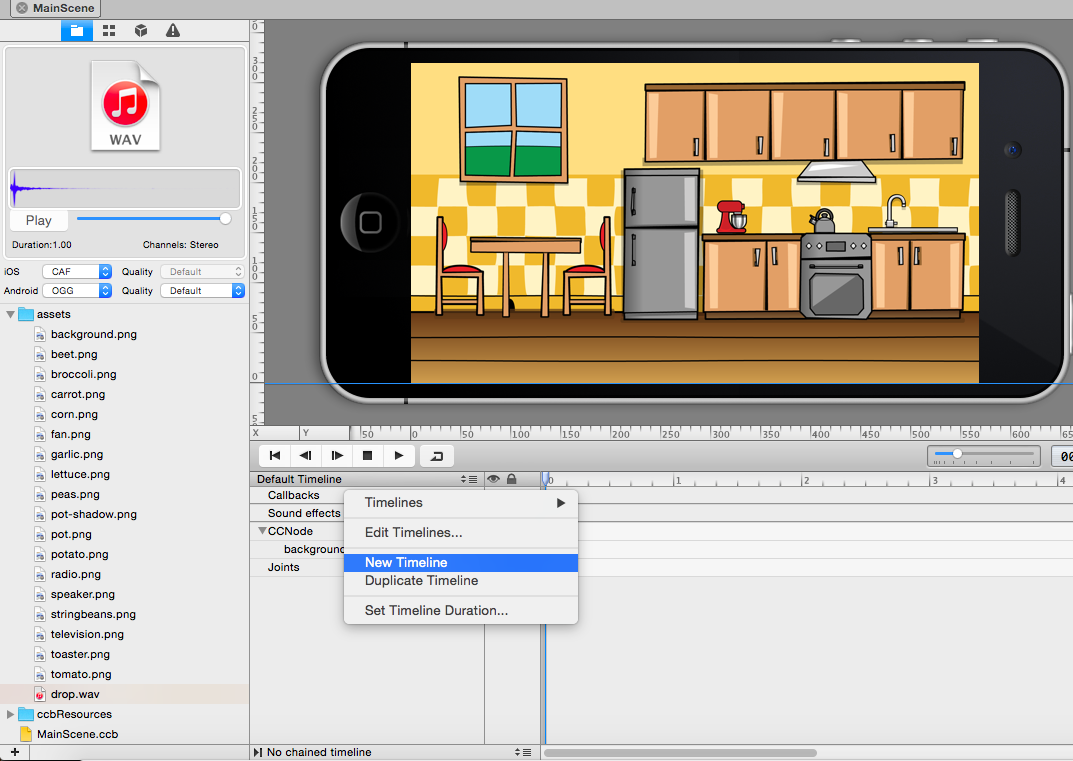
\includegraphics[width=0.9\linewidth]{images/Chapter2/new_timeline_audio.png}
		\caption{WAV files can be added by dragging them to the resource
		pane}\label{fig:audio_new_timeline}
\end{figure}

There are different ways to play sound effects added to your \SB{} project: you
can add a sound effect to a \SB{} timeline or you can play a sound effect
directly from code. We will first look at the timeline approach, implementing the code
approach will be an exercise at the end of this chapter. Before we set up the
sound effect I want to give you a basic introduction to the timeline feature
of \SB{} since it is one of the most important ones!

\subsection{\SB{}'s timeline feature}\index{\SB{} timeline}
The \SB{} timeline is a tool that allows developers to create animations and
sequences of sound effects without writing code. Every \ccbfile{} has one
\textit{Default Timeline} associated with it as soon as it is created. However,
a \ccbfile{} can, and often will, have multiple different timelines. Each
timeline is a sequence of sound effects, callbacks and most importantly
keyframes.

\ldots

%TODO: discuss keyframes, sound effects, callbacks, autoplay, etc.

\subsubsection{Adding the sound effect to a timeline}

Start by creating a new timeline for the sound effect as show in figure
\ref{fig:audio_new_timeline}. Once the timeline is created you can drag the
sound effect from the asset library in the left panel to the \textit{Sound
effects} row of \SB{}'s timeline (the second row from the top).

\begin{figure}[H]
		\centering
		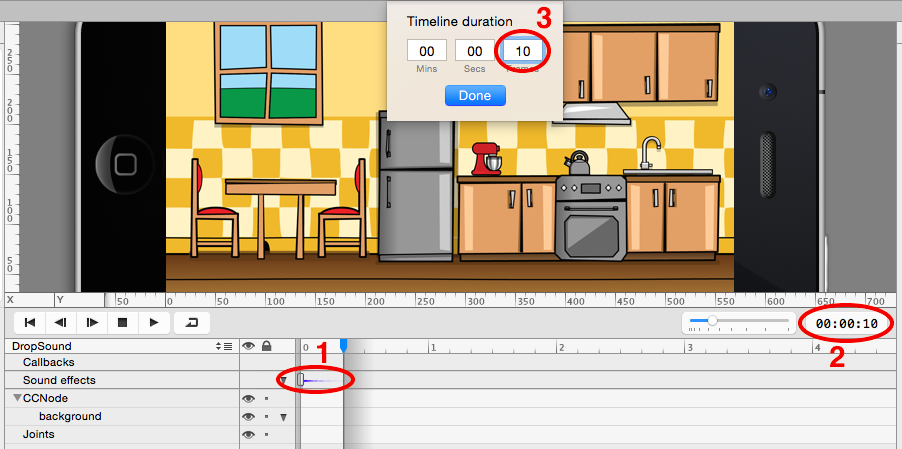
\includegraphics[width=0.9\linewidth]{images/Chapter2/audio_timeline.png}
		\caption{(1) Audio file added to timeline\newline{} (2)
		Button to change timeline duration\newline{} (3) Timeline
		duration dialog\newline{}}\label{fig:change_timeline_duration}
\end{figure}

When the sound is added to the timeline it will be displayed in wave form. You
should adjust the duration of the timeline to match the duration of the sound
effect. Figure \ref{fig:change_timeline_duration} shows how you can change the
duration. You should set it to 10 frames.

Now the sound is ready to play! The last step is assigning a unique name to this
timeline which we can reference from code. You can rename a timeline by either
choosing \textit{Animation -> Edit Timelines\ldots} or selecting the dropdown
button next to the timeline name:

\begin{figure}[H]
		\centering
		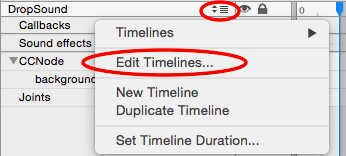
\includegraphics[width=200pt]{images/Chapter2/edit_timeline.png}
		\caption{\textit{Edit Timelines\ldots} allows you to change the name of a
		timeline}
\end{figure}

I have chosen \textit{DropSound} for the name of this timeline. Now everything
is set up and you can hit the publish button in \SB{}.

\subsection{Triggering a Sound Effect}
Now we have set up the sound effect in \SB{} and published the project, all that
is left to do is to open the \xcode{} project and play the sound effect as soon
as an object falls below the screen boundary.

We are going to implement this in \textit{SBBMainScene.m}. \cocos{} provides a
very simple API call to run a timeline animation from code. The following line
added to \inlinecode{SBBMainScene} will run the timeline animation and thus play the
sound we added to the project:
\begin{lstlisting}
animationManager.runAnimationsForSequenceNamed("DropSound")
\end{lstlisting}
The animation manager of the root node of a \ccbfile{} provides us access to the
different timelines and allows us to run, pause them and to react to their
completion - we will use these capabilities extensively throughout this book.

As mentioned earlier we want to play the sound effect when an object falls off
the screen. We already have code that checks for that condition in our
\inlinecode{update} method, all we need to do this to add the line that runs the
timeline. Extend the relevant part of the \inlinecode{update} method to look as
following:
\begin{lstlisting}
// check if falling object is below the screen boundary
if (CGRectGetMaxY(fallingObject.boundingBox()) < CGRectGetMinY(boundingBox())) {
	// if object is below screen, remove it
    fallingObject.removeFromParent()
    fallingObjects.removeAtIndex(i)
    // play sound effect
    animationManager.runAnimationsForSequenceNamed("DropSound")
} else {...}
\end{lstlisting}
Now you can compile and test the project. Every time an object falls of the
screen you should hear the drop sound play!
\section{Wrapping up}
In this chapter you have learned how to work with an essential component of all
video games - image and audio assets. You have learned how to design scenes with
sprites in \SB{}, how to load and change sprite textures in code. You got to
know how \SB{} handles different asset resolutions for different screen and
device types and you have played your first sound effect. You have learned some
of the most important essentials of game development with \SB{} and \cocos{}.

The focus of the next chapter is \textit{User Interaction}. You will learn how
to implement Drag and Drop functionality, how to use the Accelerometer as an
alternative control scheme and how to use gestures to make your games more
enjoyable. Before you move on you should complete the exercise for this chapter.

\section{Exercises}
Now it's time for an exercise. For this exercise you will have to use internet
research.
\begin{description}
\item[2.0] Play the 'drop' sound without using a \SB{} timeline. Tips: you will
have to use \inlinecode{OALSimpleAudio} to play the sound and
\inlinecode{CCFileUtils} to find the location of the sound file. Note that this
approach that avoids using a \SB{} can often be the more convenient approach to
playing sound effects in your game!
\end{description}
\chapter{User Interaction and Collision Detection}

In this chapter you will incorporate User Interaction into the object catching
game. The first step will be implementing a drag and drop mechanism that lets
the user move the pot in order to catch objects. To detect if the player has
caught or missed an object we will implement basic collision detection - note
that you will later learn how to use the \cocos{} physics engine that provides
collision detection out of the box. Whether you want to implement your own
collision detection or use the physics engine will depend a lot on the type of
game you are developing and we will discuss the advantages of both approaches
throughout this book.

When we've implemented the first control scheme we will add a second option for
players - controlling the game with the accelerometer of the device, another
common way to interact with mobile games.

As a byproduct of implementing these features we will work with translating
positions and sizes between different node spaces and the world space, so we
will be discussing that important concept throughout this chapter as well.

\section{Add the pot to the game}
The goal of our game will be to move a pot across the screen and try to catch
all the vegetables while avoiding catching inedible objects. Before we can
implement the drag and drop mechanism we need to add the pot assets to our game,
we're going to do that in the \SB{} project, open it now.

Typically we use individual \ccbfile{}s for each type of object in our game,
however for this game we need to make an exception due to the specific way in
which order \cocos{} renders our objects in the game.

\subsection{Working with the z-order}\index{Z-Order}
Throughout this book we are working with a 2D engine. In a 2D engine depth can
only be represented by certain objects being placed in front or behind of other
objects. \cocos{} uses the following criteria to decide which nodes are rendered
in front of other nodes:
\begin{enumerate}
  \item Child nodes are rendered in front of their parent nodes
  \item Siblings (nodes with the same parent) are rendered in order of their
  \inlinecode{zOrder} property; nodes with higher \inlinecode{zOrder} are
  rendered in front of nodes with a lower one
  \item If two siblings have the same \inlinecode{zOrder} the siblings are
  rendered in reverse order of how they have been added (the latest added node
  is rendered in front of all other nodes)
\end{enumerate}

As you can see from the description above the \inlinecode{zOrder} only affects
how siblings are ordered, \cocos{} currently does not have a global
\inlinecode{zOrder}. For our game we want to create the illusion of objects
dropping into a pot, we can do that using the \cocos{} Z-order as shown in
the figure below. 

\begin{figure}[H]
		\centering
		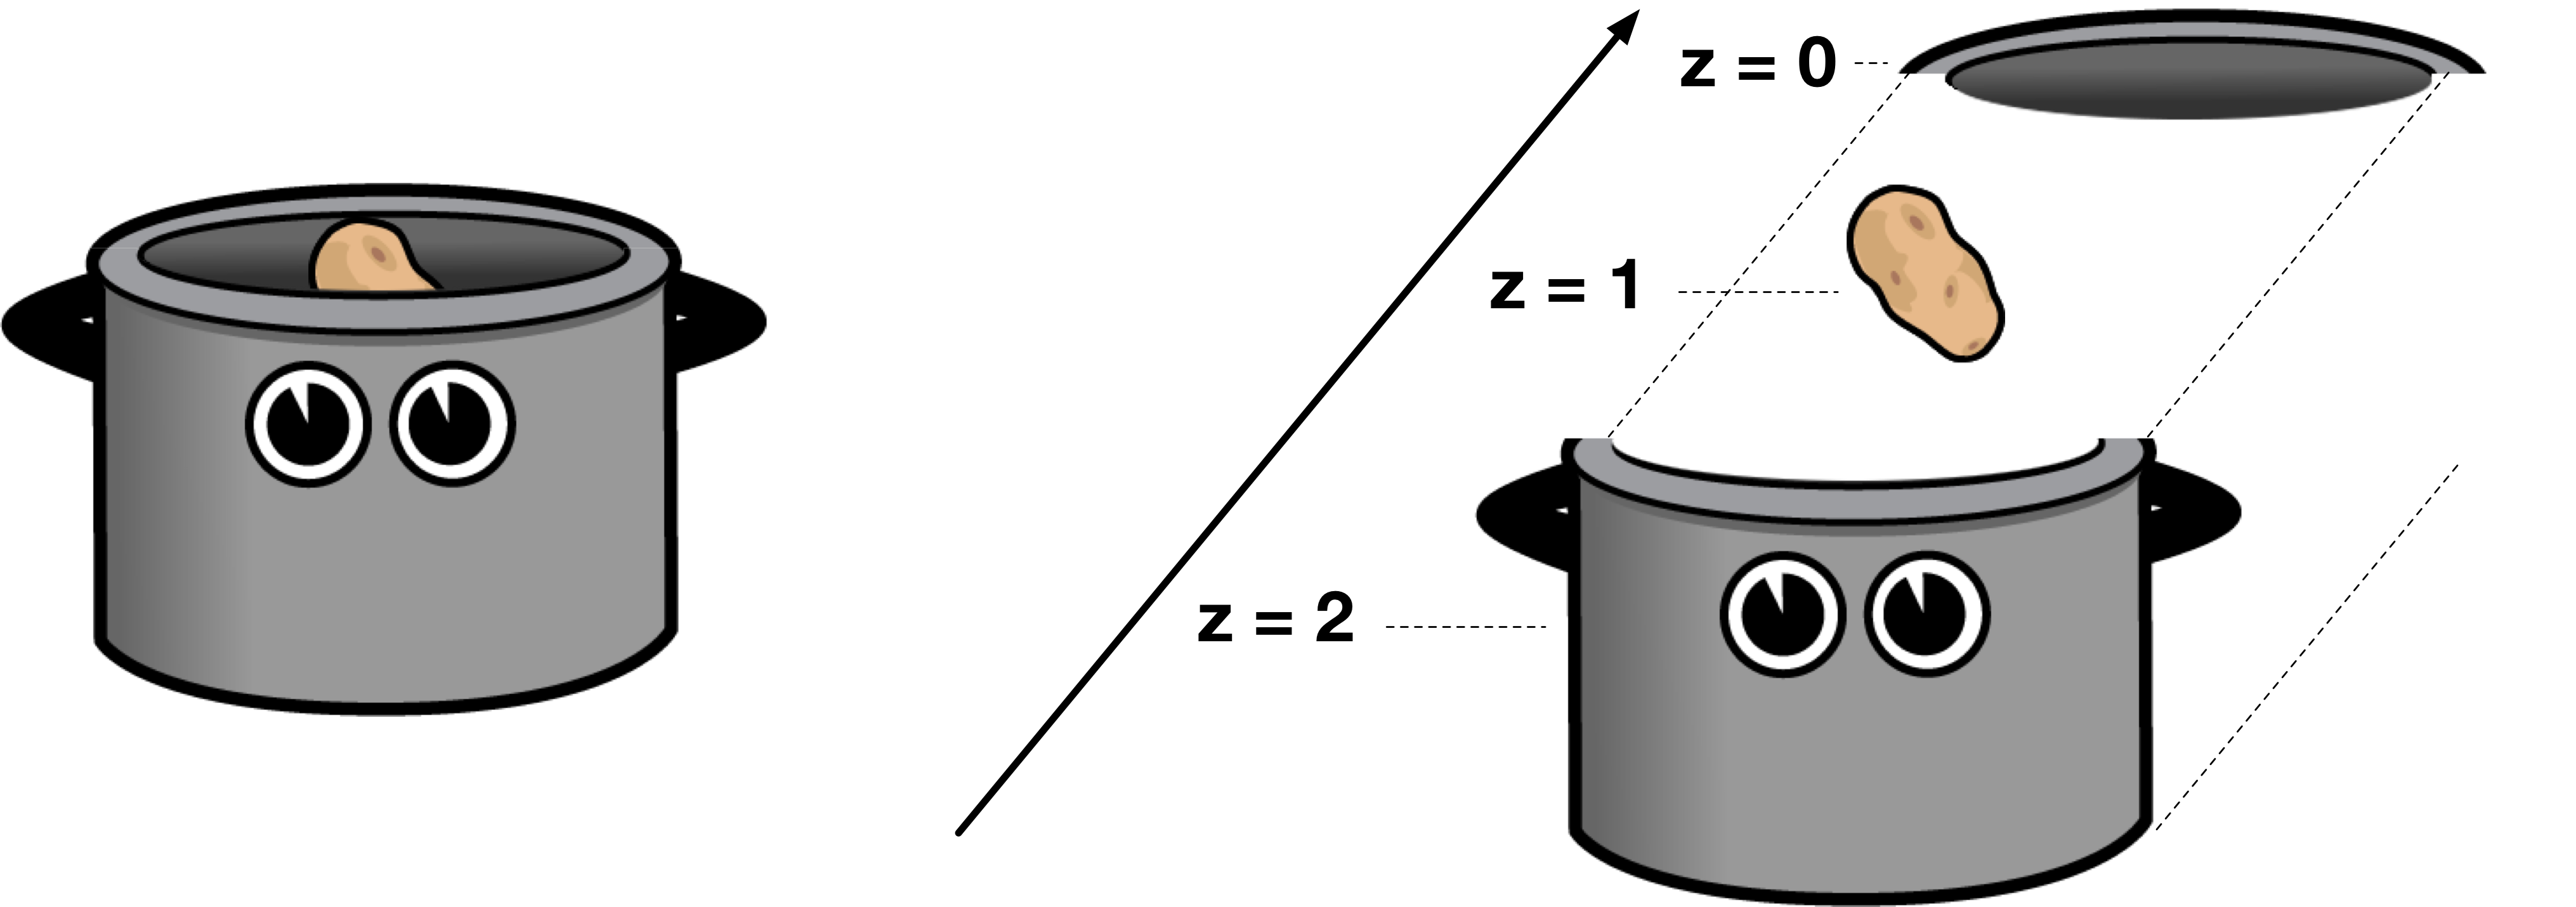
\includegraphics[width=0.9\linewidth]{images/Chapter3/drawing_order.png}
		\caption{Left: Objects on different Layers, Right: How the Z-Order influences
		on which Layer a node is rendered}
\end{figure}

For this solution to work all the falling objects and the bottom and top part of
our pot need to have the same parent node, otherwise we would not be able to use
the Z-Order to place the falling objects between the two parts of the pot. 

That is the reason why we are not creating a separate \ccbfile{} for the pot
object and instead place it inside of \inlinecode{MainScene.ccb}. There would be
other ways to work around this issue but adding the pot to the Main Scene is a
good solution for this game.

\begin{details}[frametitle={Global Z-order in \cocos{}}] 
While \cocos{} does not have support for global Z-order at the moment, it is
being discussed as a potential feature for future releases. Many games run into
issues as discussed above due to the lack of this feature. You can follow the
discussion on GitHub: \url{https://github.com/cocos2d/cocos2d-swift/issues/662}.
\end{details}

\subsection{Setting up the pot assets}
Equipped with everything we need to know about Z-order let's add the pot assets
to our Main Scene in \SB{}:

\begin{figure}[H]
		\centering
		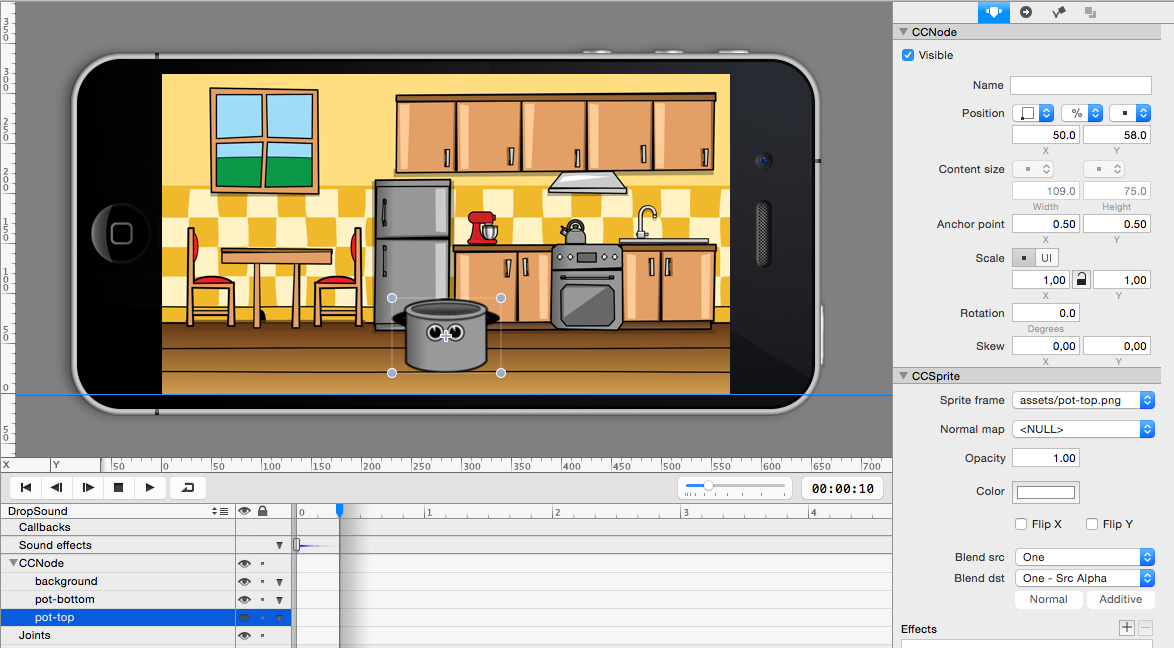
\includegraphics[width=0.9\linewidth]{images/Chapter3/add_pot.png}
		\caption{Add both pot parts to the main scene}
\end{figure}

\begin{leftbar}
The assets of both pot parts have exactly the same dimensions.
 Place both of them at 50\% X position and at a Y position of 58
Create code connections for both pot parts, linked to the \textit{Document Root}. 
Name them \inlinecode{potBottom} and \inlinecode{potTop} respectively.
Publish the \SB{} project
\end{leftbar}

Next, move to the \xcode{} project to set up the code connection variables and
implement the touch handling code.

\begin{leftbar}
Open \inlinecode{MainScene.swift} and add instance variables for our code
connections at the top of the class:
\begin{lstlisting}
weak var potTop: CCSprite!
weak var potBottom: CCSprite!
\end{lstlisting}
\end{leftbar}
There are three important things to remember about these code connections.
Firstly, all code connections should be marked as \inlinecode{weak}.
\inlinecode{MainScene} has a reference to the pot sprites but does not
\textit{own} them. Instead they are owned by their parent node. For any
references that don't mark an ownership, \inlinecode{weak} should be used. 

Secondly, we always want to declare code connections as \textit{forcefully
unwrapped optionals} as denoted by the bang (!) after the type. Swift
requires that all instance variables that aren't optionals are either
initialized with a default value or get set to a value in one of the
initializers of the class, that way the compiler can guarantee that these
variables never contain a \inlinecode{nil} value. Code connections however are
set up after the object is initialized (they are guaranteed to be set up
when \inlinecode{didLoadFromCCB} is called on the node), so technically these
should be optional values. Adding a lot of code for \inlinecode{nil} checking
would clutter our classes, that's why we prefer using the bang notation which
basically says: \textit{I am confident that this value will never be nil when I
am trying to access it}. This is true for code connections as we now that
\cocos{} guarantees to have set them up by the time \inlinecode{didLoadFromCCB}
is called.

Lastly, be careful not to mark these variables as \inlinecode{private}.
Otherwise \cocos{} will not have access to them and won't be able to set up the
code connections.

Okay, now we have the basics set up and are ready to dive into the details of
implementing a drag and drop mechanism!

\section{Implement a Drag and Drop mechanism}
For the very first project in this book we have already implemented a basic
touch mechanism. You should remember that \inlinecode{userInteractionEnabled} is
the property that activates/deactivates touch handling for a node and that
\cocos{} provides four different callbacks for different state transitions in
the lifecycle of a touch. Here's the recap:

\begin{description}
\item[touchBegan:] called when a touch begins
\item[touchMoved:] called when the touch position of a touch changes
\item[touchEnded:] called when a touch ends because the user stops touching the
screen
\item[touchCancelled:] called when a touch is cancelled because user moves touch
outside of the touch area of a node
\end{description}

Knowing that, how can we implement a drag and drop control scheme for our game?
Dragging and dropping includes three different steps:
\begin{enumerate}
  \item Pick up object
  \item Drag object
  \item Drop object
\end{enumerate}

\subsection{Picking up an Object}
In order to pick up an object we need to detect a user's touch and determine if
the touch is within the boundaries of our object, if that is the case,
we start dragging the object.

First of all, let's turn on user interaction for the \inlinecode{MainScene}
class, so that we receive touch events.

\begin{leftbar}
Add the required line to the \inlinecode{onEnterTransitionDidFinish} method:
\begin{lstlisting}
  override func onEnterTransitionDidFinish() {
    super.onEnterTransitionDidFinish()
    
    self.userInteractionEnabled = true
    
    // spawn objects with defined frequency
    schedule("spawnObject", interval: spawnFrequency)
  }
\end{lstlisting}
\end{leftbar}

Next, we need to add the touch handling method. The touch handling method will
need to check if the touch is within our pot. If that is the case, the method
will need to set a state variable that remembers that we are currently dragging
this object. If the user moves a finger across the screen and we are currently
in object dragging mode, it is important that the object follows the finger of
the user.

\begin{leftbar}
Add this implementation to \inlinecode{MainScene.swift}:
\begin{lstlisting}
  override func touchBegan(touch: CCTouch, withEvent event: CCTouchEvent) {
    if (CGRectContainsPoint(potBottom.boundingBox(), touch.locationInNode(self))) {
      isDraggingPot = true
      dragTouchOffset = ccpSub(potBottom.anchorPointInPoints, touch.locationInNode(potBottom))
    }
  }
\end{lstlisting}
\end{leftbar}

Let's discuss this implementation briefly. You already have seen the usage of 
\inlinecode{touch.locationInNode(self)} in the first chapter of this book,
where we briefly discussed touch handling
(\ref{Introduction_FirstTouchHandling}). This method returns the touch position
within a given node. In this specific case we are receiving the touch position
within \inlinecode{MainScene}.

Next, we are using a utility function, \inlinecode{CGRectContainsPoint}, to
check if this touch is within the pot. Remember,
that \inlinecode{potBottom} and \inlinecode{potTop} are placed at exactly
the same position, so we can choose either of them for this check.
\inlinecode{CGRectContainsPoint} takes a rectangle as its first argument and a
point as its second. It returns true if the point is within the rectangle.

If the touch position is inside of the pot, we set our state variable,
\inlinecode{isDraggingPot}, to \inlinecode{true}. 

There is one last line that we didn't discuss upfront:
\begin{lstlisting}
dragTouchOffset = ccpSub(potBottom.anchorPointInPoints, touch.locationInNode(potBottom))
\end{lstlisting}

In order to drag an object smoothly we need to remember where we touched that
object when starting dragging. Take a look at the following diagram:
\begin{figure}[H]
		\centering
		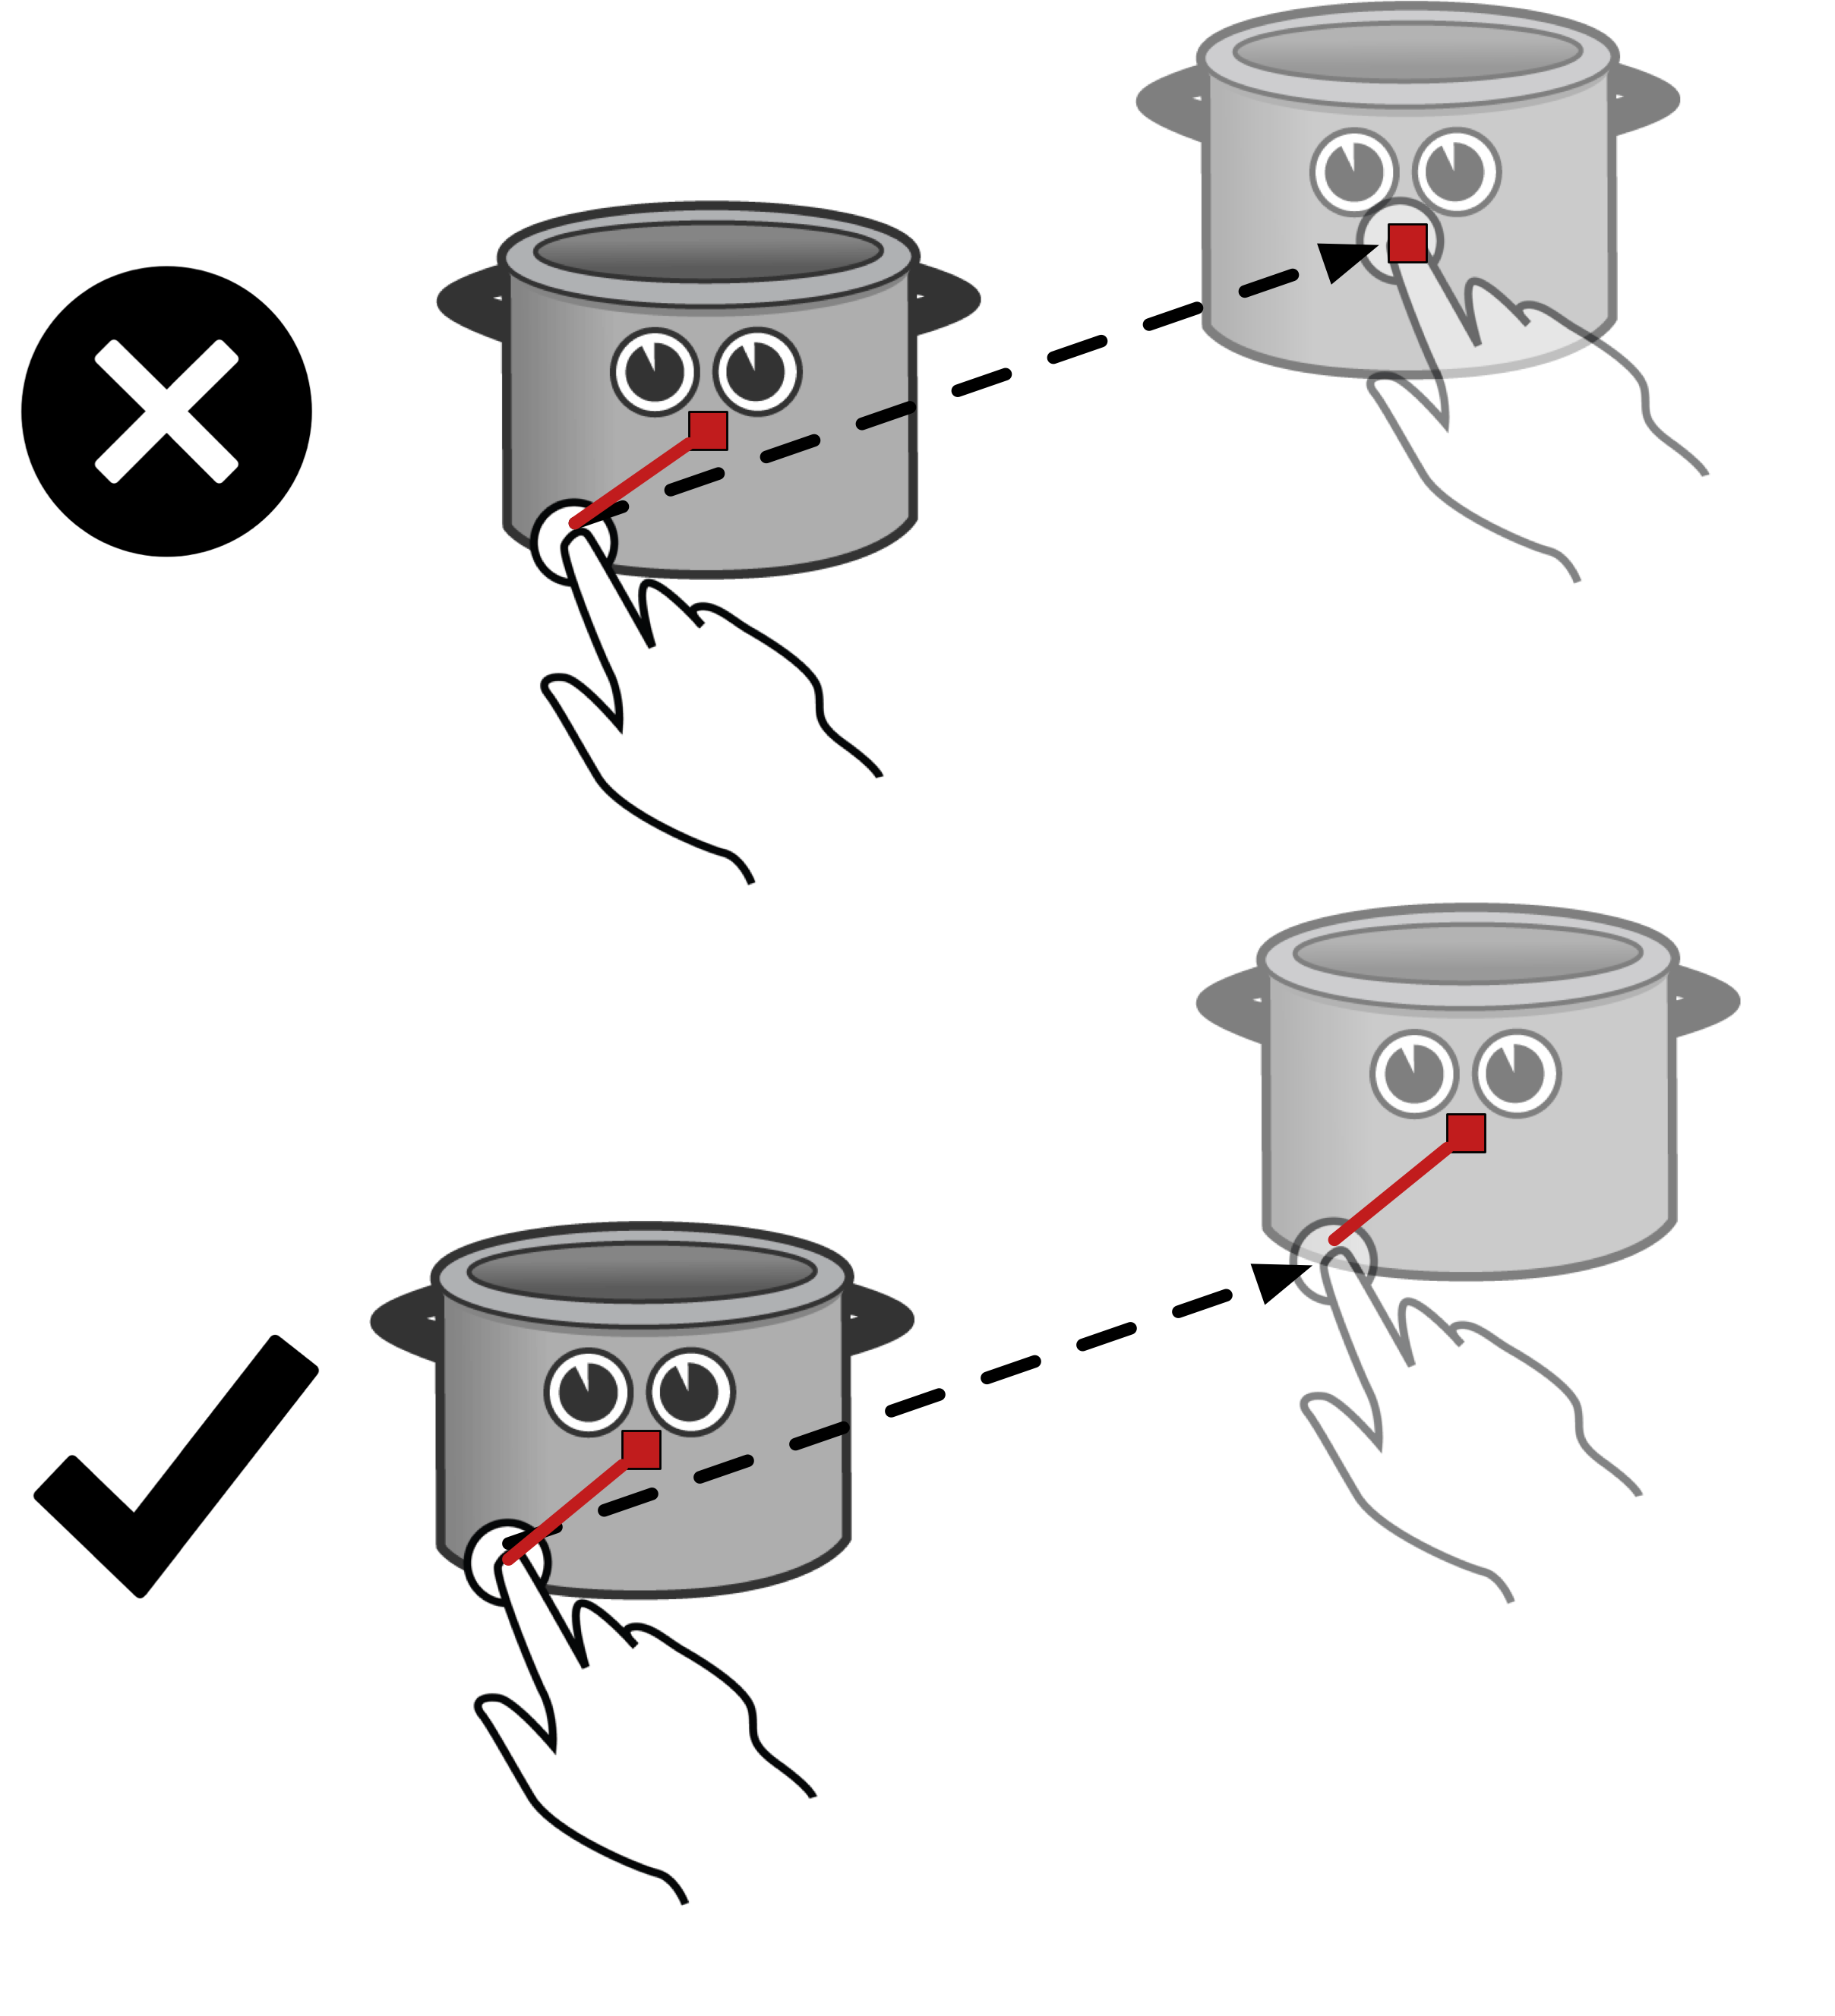
\includegraphics[width=0.4\linewidth]{images/Chapter3/dragging_offset.png}
		\caption{\textit{Top Image:} incorrect implementation, object jumps to touch
		position. \textit{Bottom Image:} correct implementation, touch offset is
		maintained while dragging the object.}
		\label{user_interaction_touch_offset}
\end{figure}
As the user moves the finger, we move the object along. However, the position of
the object is not exactly the touch position. Instead it is the touch position
\textit{plus} the touch offset determined when we started dragging. We determine
that offset by calculating the distance between the anchor point (that's the
reference point for positioning a node, typically it's in the center of the
node) of the touched object and the exact touch position. 
No we know why it is important to store the touch offset!

\begin{leftbar}
To wrap up the implementation of \inlinecode{touchBegan} let's add the two
instance variables we have referenced: \inlinecode{isDraggingPot} and
\inlinecode{dragTouchOffset}. Your list of iVars should now look like this:
\begin{lstlisting}
  weak var potTop:CCSprite!
  weak var potBottom:CCSprite!
  
  private var fallingObjects = [FallingObject]()
  private let fallingSpeed = 100.0
  private let spawnFrequency = 0.5
  private var isDraggingPot = false
  private var dragTouchOffset = ccp(0,0)
\end{lstlisting}
\end{leftbar}

\subsection{Moving an Object}
Now we'll implement the code that actually moves the pot. That code needs to run
whenever a user's finger moves. That means we need to implement the
\inlinecode{touchMoved} method.
\begin{leftbar}
Add the \inlinecode{touchMoved} method below the \inlinecode{touchBegan} method:
\begin{lstlisting}
  override func touchMoved(touch: CCTouch, withEvent event: CCTouchEvent) {
    if (!isDraggingPot) {
      return
    }
    
    var newPosition = touch.locationInNode(self)
    // apply touch offset
    newPosition = ccpAdd(newPosition, dragTouchOffset);
    // ensure constant y position
    newPosition = ccp(newPosition.x, potBottom.positionInPoints.y);
    // apply new position to both pot parts
    potBottom.positionInPoints = newPosition;
    potTop.positionInPoints = newPosition;
  }
\end{lstlisting}
\end{leftbar}
In the first line we check if we are currently in dragging mode. If not, we do
nothing and return immediately. This prevents the pot from jumping to the latest
touch position if it has not been picked up beforehand.

If we are in dragging mode we continue. First we get the new touch position.
Then we apply the offset that we discussed in figure
\ref{user_interaction_touch_offset} to that new position. The next line ensures
that the y position of the pot stays constant, we want to allow horizontal
movement only. Finally, we apply that new position to both pot parts. Great,
we're pretty close to finishing the drag and drop functionality.

If you test the app in the current state you'll see that there's one simple yet
important step missing\ldots

\subsection{Dropping an object}
Right, the user will also want to drop the pot by releasing the finger from the
screen. Otherwise we stay in dragging mode forever and the pot will keep jumping
to whichever position the user taps on the screen.

Luckily this can be easily implemented. All we need to do is to set
\inlinecode{isDraggingPot} to false as soon as the user stops touching the
screen.
\begin{leftbar}
Add the \inlinecode{touchEnded} method below the \inlinecode{touchMoved} method:
\begin{lstlisting}
  override func touchEnded(touch: CCTouch, withEvent event: CCTouchEvent) {
    isDraggingPot = false
  }
\end{lstlisting}
\end{leftbar}
Awesome! Our drag and drop code is complete! Drag and drop mechanisms can be
used in many types of games, so what you have learned in this chapter is very
valuable.

Now we can move on to the hardest (thus most interesting) part of this chapter
- catching objects.

\section{Catching objects}
Implementing drag and drop was a great warm up. In this section we are going to
solve a bunch of problems that will bring our little project a large step closer
to being a real game. By the end of this section the user will be able to catch
and miss objects by dragging the pot below objects with the right timing.

Before we dive into coding let's think about what we actually need to implement.
There are three important aspects that need to be covered through our
implementation:
\begin{enumerate}
  \item detecting if the user has caught an object
  \item detecting if the user has missed an object
  \item visualizing catching / missing correctly
\end{enumerate}

\subsection{Thinking in states}
Our feature outline describes that objects start out as falling objects,
directly after they have been spawned. At some later point in time the user can
catch or miss these objects. In each of these situations we need our falling objects to behave differently. If they are
falling we want them to move down the screen with a constant speed. If they are
caught we need some sort of visualisation - ideally the objects move into the
pot and disappear. If the user tries to catch an object too late and misses it
closely we want to visualize that, too.

From the paragraph above we can extract three different states in which a
falling object can be:
\begin{figure}[H]
		\centering
		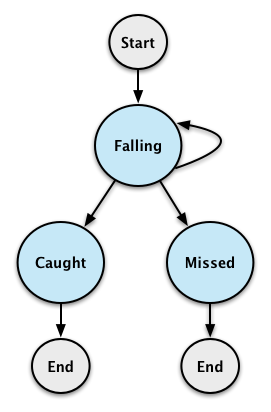
\includegraphics[width=0.3\linewidth]{images/Chapter3/falling_object_states.png}
		\caption{Objects start in falling state, then they end up caught or missed}
\end{figure}
As the diagram shows, a falling object can either stay a falling object or turn
into a caught or missed object. It is up to us developers to decide the criteria
for a state change. We also need to decide when we want to check for state
changes.

For our game I suggest that we check whether a player has caught an object or
not in the \inlinecode{update} method. As soon as that object reaches the y
position of the top of the pot we decide based on the x position whether the
object has been caught or missed 
\begin{figure}[H]
		\centering
		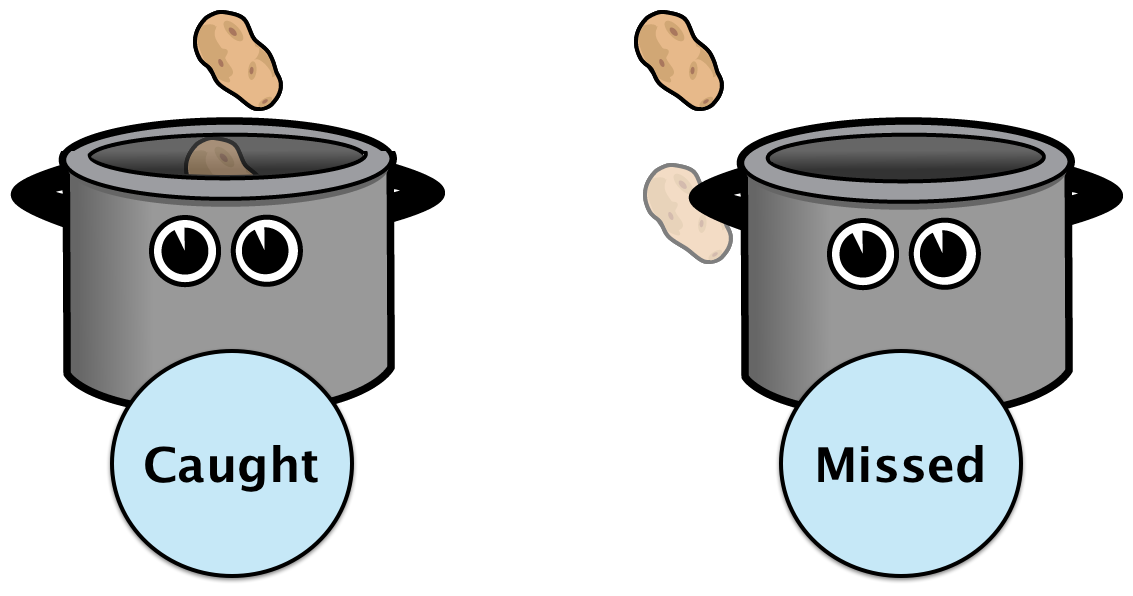
\includegraphics[width=0.3\linewidth]{images/Chapter3/catch_test.png}
		\caption{Caught objects fall into the pot, missed objects fall behind}
		\label{CaughtMissedDefinition}
\end{figure}
Since we are building a 2D game we only have limited ways of expressing that a
player missed a falling object - I suggest that we render missed objects behind
the pot. That way players can quickly see whether they caught an object or not.

Now we have a good starting point for some coding; we need to store
different states for falling objects and we need to write specific behavior
code for each of these states. Additionally we need to write code that checks if
we have caught or missed an object so that we can assign the correct states to
falling objects.

\subsection{Storing state}
Now we'll start implementing everything described earlier. Let's start by adding
a \inlinecode{fallingState} to \inlinecode{FallingObject.swift}. That state
variable will remember whether an object is currently falling, has been caught
or has been missed.

The best way to represent states in Swift is to use an enumeration!
\begin{leftbar}
Add this enum definition to \inlinecode{FallingObject.swift} below the
\inlinecode{FallingObjectType} enum:
\begin{lstlisting}
  enum FallingObjectState {
    case Falling
    case Caught
    case Missed
  }
\end{lstlisting}
\end{leftbar}
As mentioned earlier, associating enum entries with a type is not
mandatory. In this case our entries don't need a type (e.g. Int) since the
entries will only represent a state - they are values in their own right.

\begin{leftbar}
Next, add an instance variable to store the current state:
\begin{lstlisting}
  var fallingState = FallingObjectState.Falling
\end{lstlisting}
\end{leftbar}
This variable should not be private, we want to change the value as
the object gets caught or missed. Our default state is \inlinecode{.Falling}, we
assign it as part of the variable declaration.

Now we can store a \inlinecode{fallingState} for each falling object; next,
let's implement different behaviour based on that state.

\subsection{Implement state specific behaviour}
The majority of our gameplay code is currently inside of the \inlinecode{update}
method of \inlinecode{MainScene}. This is fairly common for simple games.
Currently we are doing to things in the update method: moving the objects down
the screen and checking whether they have left the stage entirely (in which
case we delete them). Now however, we are going to add code that will only run
for falling objects in certain states. That will add quite a lot of complexity.
Instead of squashing everything into the update method I suggest that we
create one method for each of the three states. These methods will contain
all state specific code and will be called from the update method.

\begin{leftbar}
Replace your existing update method with the following one:
\begin{lstlisting}
    override func update(delta: CCTime) {
    // use classic for loop so that we can remove objects while iterating over the array
    for (var i = 0; i < fallingObjects.count; i++) {
      let fallingObject = fallingObjects[i]
      
      // let the object fall with a constant speed
      fallingObject.position = ccp(
        fallingObject.position.x,
        fallingObject.position.y - CGFloat(fallingSpeed * delta)
      )
      
      switch fallingObject.fallingState {
      case .Falling:
        performFallingStep(fallingObject)
      case .Missed:
        performMissedStep(fallingObject)
      case .Caught:
        performCaughtStep(fallingObject)
      }
    }
  }
\end{lstlisting}
\end{leftbar} 
Now the update method is really easy to read. We loop over all falling objects.
In all cases we move the falling object towards the bottom of the screen. After
that we check in which state an object is and invoke a method that contains code
specific for that state. We are going to implement these methods throughout the
remainder of this chapter.

\subsection{Implementing the falling state}
Let's start implementing the default state: falling. In this state we will need
check whether an object has been caught, has been missed or simply remains
falling. 

Later in this book you will learn how to use the \cocos{} physics
engine and its built in collision detection - for this game however we are not
using the physics engine and will implement catch detection code ourselves.

In figure \ref{CaughtMissedDefinition} we have illustrated what we consider a
caught/missed object. So how can we implement this? Basically all we need to do
is compare the frame of the falling object to the frame of the pot. However,
there is one small issue. The frame of \ccsprite{} is always a rectangle that
contains the entire texture, here's what the dimensions of the frames of our pot
and a falling object looks like:
\begin{figure}[H]
		\centering
		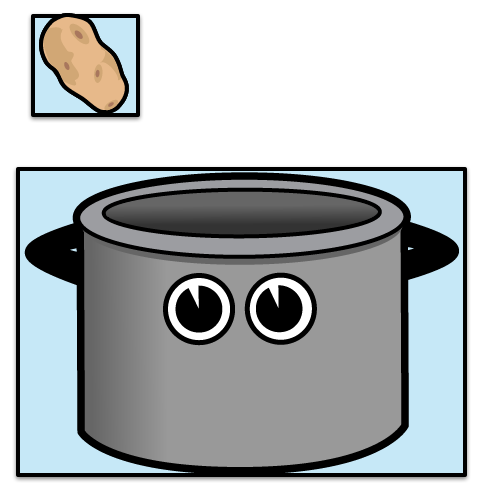
\includegraphics[width=0.3\linewidth]{images/Chapter3/frame_pot_falling_object.png}
		\caption{The pot frame is too large to use it for collision detection}
\end{figure}
From the illustration above you can see that the frame of the pot is too large
to use it for collision detection. It could easily happen that an object
landing on the handle of the pot would still be considered a catch.

Instead of using the pot dimensions we will need to add a separate, smaller,
node in \SB{} that marks the catch area. 
\begin{leftbar}
Open the \SB{} project and open \filemention{MainScene.ccb}.
\ldots
Now publish the \SB{} project and switch back to the \xcode{} project.
\end{leftbar}
Next, we need to add a variable for the code connection we just set up.
\begin{leftbar}
Add the catch container variable to the other code connection variables:
\begin{lstlisting}
weak var catchContainer: CCSprite!
\end{lstlisting}
\end{leftbar}
Now we have a reference container set up that will allow us to test if objects
have been caught. We can start implementing falling step function.
\begin{leftbar}
Add the method stub for the falling step to \filemention{MainScene.swift}:
\begin{lstlisting}
  func performFallingStep(fallingObject:FallingObject) {

  }
\end{lstlisting}
\end{leftbar}
Before we can dive into collision detection we will have to take a little detour
and talk about node transformations.\index{Node transformation!Bounding Box} As
part of the introduction to \cocos{} we have discussed that nodes are always positioned
relative to their parent node (chapter: \ref{Introduction_CCNode}). The catch
container that we just added in \SB{} is a child of the \inlinecode{potBottom}
node. We chose that setup so that the catch container always moves together
with the pot. 

For our collision detection algorithm we want to compare the position of a
falling object to the position of our catch container. \textbf{Here the problem
arises: falling objects and the catch container have different parent nodes,
that means we cannot compare their positions and frames directly.} Since the
position is relative to the parent node, comparing nodes with different parents
would resolve in unexpected behavior. Take the following illustration as an
example:
\begin{figure}[H]
		\centering
		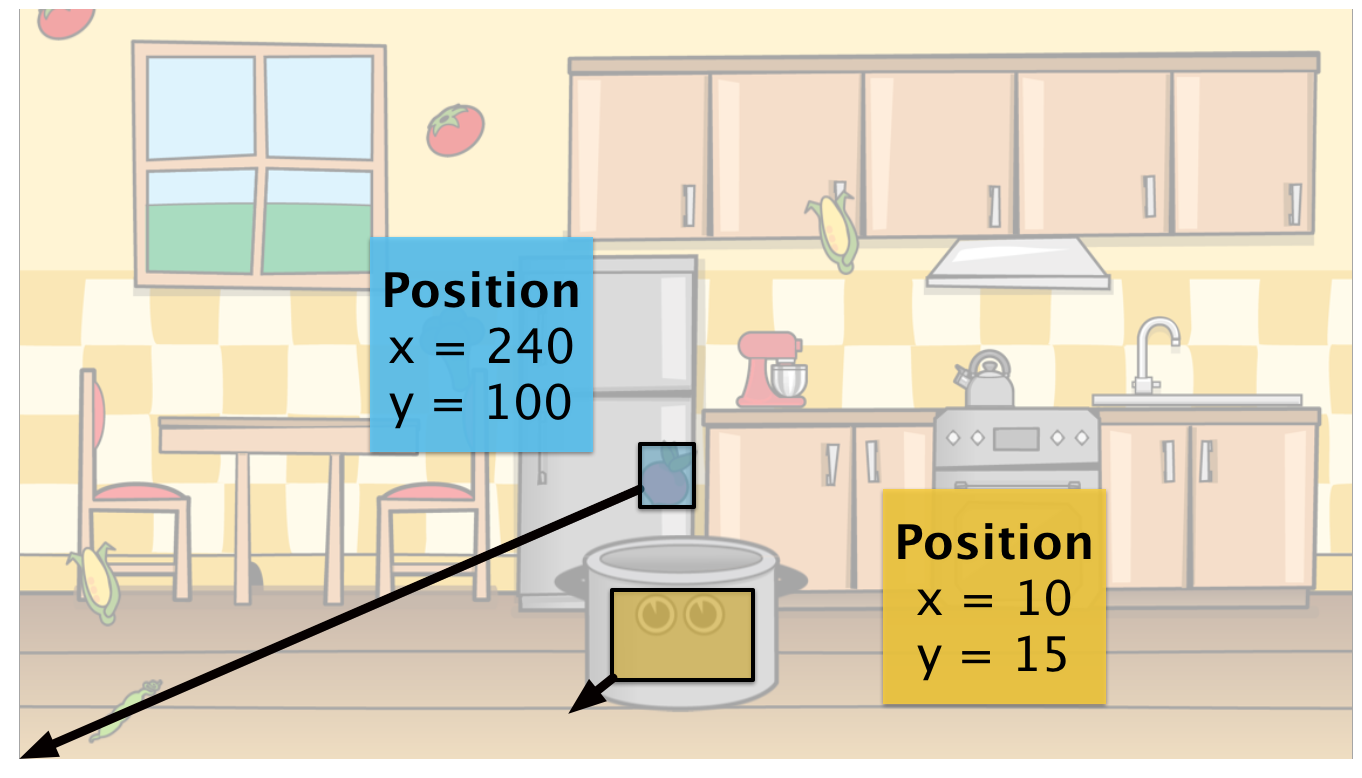
\includegraphics[width=0.7\linewidth]{images/Chapter3/parent_transform.png}
		\caption{Even though the two nodes illustrated above are close to each other,
		their position values are entirely different, since they are placed relative
		to different parents}
\end{figure}
How can we work around this? Luckily \cocos{} exposes a couple of variables and
methods that allows us to transform positions and frames between different
\textit{node spaces}. Each node lives in the \textit{node space} of its parent.
In our example the catch container is in the node space of the pot and the pot is
in the node space of the main scene.

If we want to know the position and size of the catching container in the main
scene node space, we need to apply the following transform:
\begin{lstlisting}
let containerWorldBoundingBox = CGRectApplyAffineTransform(
  catchContainer.boundingBox(), catchContainer.parent.nodeToParentTransform()
);
\end{lstlisting}
We are transforming the bounding box of the catch container using the
\inlinecode{nodeToParentTransform} of the catch container's parent node (the
pot). The \cocos{} documentation describes the
\inlinecode{nodeToParentTransform} as following: \textit{Returns the matrix that
transform the node's (local) space coordinates into the parent's space coordinates.}

This means after applying the transform we know the position of the catch
container in the main scene space. 

If you are new to graphics programming this concept will likely seem a little
confusing; frankly you won't need it too often when working with \cocos{}. If
you aren't getting a hold of transforms yet, don't worry too much!

\begin{details}[frametitle={The role of transforms in graphics programming}]
Transforms are an essential part of all graphics engines - also of \cocos{}.
When determining the positions for all nodes in a scene, \cocos{} starts with
the root node. After the root node is laid out, the engine moves to the children
of the root node, calculates their position and places them \textit{relative to
the root node}. This is repeated all the way down the node hierarchy:
\begin{figure}[H]
		\centering
		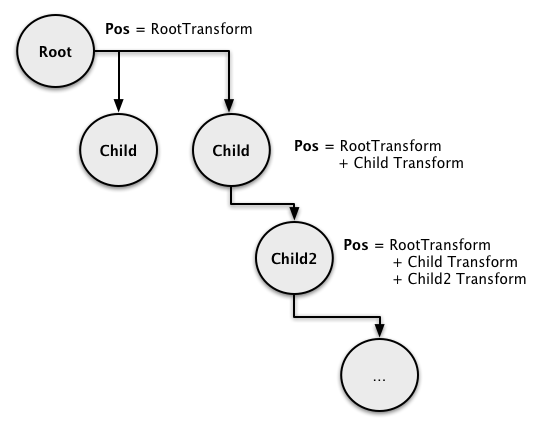
\includegraphics[width=0.5\linewidth]{images/Chapter3/parent_transform_rendering.png}
\end{figure}
\end{details}

Now that we have a solution for the transformation issue, the rest of the
code that we need for the falling step is not too complicated.
\begin{leftbar}
Here's the entire function that implements the stub that you added earlier:
\begin{lstlisting}
  func performFallingStep(fallingObject:FallingObject) {
    let containerWorldBoundingBox = CGRectApplyAffineTransform(
      catchContainer.boundingBox(), catchContainer.parent.nodeToParentTransform()
    );
    
    let yPositionInCatchContainer = CGRectGetMinY(fallingObject.boundingBox()) < CGRectGetMaxY(containerWorldBoundingBox)
    let xPositionLargerThanLeftEdge = CGRectGetMinX(fallingObject.boundingBox()) > CGRectGetMinX(containerWorldBoundingBox)
    let xPositionSmallerThanRightEdge = CGRectGetMaxX(fallingObject.boundingBox()) < CGRectGetMaxX(containerWorldBoundingBox)
    
    // check if falling object is inside catching pot, trigger this when object reaches top of pot
    if (yPositionInCatchContainer) {
      if (xPositionLargerThanLeftEdge && xPositionSmallerThanRightEdge) {
          // caught the object
          let fallingObjectWorldPosition = fallingObject.parent.convertToWorldSpace(fallingObject.positionInPoints)
          fallingObject.removeFromParent()
          fallingObject.positionInPoints = potTop.convertToNodeSpace(fallingObjectWorldPosition)
          potTop.addChild(fallingObject)
          fallingObject.fallingState = .Caught
      } else {
        fallingObject.fallingState = .Missed
      }
    }
  }
\end{lstlisting}
\end{leftbar}

We have already discussed the first statement extensively, we transform the
bounding box of our catch container. That allows us to compare its position to
the position of falling objects. 

The next three lines are each used to
determine if the falling object is within the relevant boundaries of our transformed catch container. The
\inlinecode{CGRectGetMin\ldots} utility functions are used to get the
lowest/highest value on a certain axis from the bounding box. These three
statements check for the conditions outlined in figure
\ref{CaughtMissedDefinition}. If all three are true the player has caught the
object.

Next, we have an if statement that combines the three boolean variables. The
first if statement checks if the falling object is in the
\textit{critical area} using the \inlinecode{yPositionInCatchContainer}
constant. Here the y position of the falling object is the only relevant metric.
If we aren't in the critical area we do nothing at all - the object is still too
far above the pot for us to decide whether the player caught it or not.

If the object is in the critical area we now need to determine if it has
been caught or missed. This is where we need the two x position variables. If
the object is outside of the bounds we set the \inlinecode{fallingState} to
\inlinecode{.Missed}.

If the object is inside of the bounds we set the \inlinecode{fallingState} to
\inlinecode{.Caught}. Additionally we need to ensure that once the object is
caught it stays within the pot. Without additional code the caught objects are
not attached to the pot. The player could move the pot left or right and the
objects would fall out to the side of the pot. As soon as an object is caught we
need to turn it into a child node of the pot, that way they will stick together.

Here we once again need a transform.\index{Node transformation!Position} We
want to turn the falling object into a child of the pot instead of being a
child of main scene. That means we are moving the object to a different node
space. We don't want the player to see this move happen; visually the object
should stay at exactly the same position. 

In such situations we need to use a two step transform. First, we need to find
the \textit{world space} position of the node that we are moving to a
different node space. The position in the world space is expressed relative to
the world root (in most cases the bottom left corner of the screen) and not
relative to the parent node. You can think of the position in world space as a
global or absolute position. We can use the world position to find the
corresponding relative position in any node space.

Let's take a look at our specific code. First we call:
\begin{lstlisting}
let fallingObjectWorldPosition = fallingObject.parent.convertToWorldSpace(fallingObject.positionInPoints)
\end{lstlisting}
This line asks: \textit{What is the global position, independent of the parent
node, of this falling object?} The node that receives this question needs to be
the parent node of \inlinecode{fallingObject}, because that is the node
responsible for placing the \inlinecode{fallingObject} node by applying its
transform.

Now that we have saved the position, we remove the node from its parent. Next we
perform the second step of the transformation:
\begin{lstlisting}
fallingObject.positionInPoints = potTop.convertToNodeSpace(fallingObjectWorldPosition)
\end{lstlisting}
This line asks: \textit{Dear pot, I have a global position for this falling
object, could you tell me what the relative position to you would need to be? I
want the falling object to remain at the same global position after adding it to
you as a child.}
After we have determined the right position we finally add the falling object to
the pot. The object will now switch to a different node space and become a child
of the pot without that the player will realize it, awesome!

This was a pretty intense implementation so here's recap what we did to
implement the code that runs while our object is in the \textit{falling state}:
\begin{enumerate}
  \item We added a catch container do define the area in which a player can
  catch objects. We did this because the frame of the entire pot is too large to
  serve as catch area
  \item We transformed this catch container from the pot space into the main
  scene space. We did that because we need the falling object and the catch
  container to be in the same space in order to compare their positions
  \item When determine that an object has been missed we set the state of the
  falling object to \inlinecode{.Missed}
  \item When we determine that an object has been caught we set the state of the
  falling object to \inlinecode{.Caught}. Additionally we add the caught object
  as a child to the pot, to ensure that the object stays within the pot after it
  has been caught. Before we add the object as a child to the pot we use a two
  way transform to figure out the position the object needs to have as a child
  of the pot node
\end{enumerate}

This concludes almost all the features we need for the \textit{falling} step.
Later we will come back for some visual tweaks but for now can move on to the
missed state. This is also a great time for a break and your favorite hot
beverage!
\subsection{Implementing the missed state}
Good news: the remain two steps are a lot simpler. The missed step only consists
of code that we have already written.
\begin{leftbar}
Add the method for the \textit{missed} step:
\begin{lstlisting}
  func performMissedStep(fallingObject:FallingObject) {
    // check if falling object is below the screen boundary
    if (CGRectGetMaxY(fallingObject.boundingBox()) < CGRectGetMinY(boundingBox())) {
      // if object is below screen, remove it
      
      fallingObject.removeFromParent()
      let fallingObjectIndex = find(fallingObjects, fallingObject)!
      fallingObjects.removeAtIndex(fallingObjectIndex)
      // play sound effect
      animationManager.runAnimationsForSequenceNamed("DropSound")
    }
  }
\end{lstlisting}
\end{leftbar}
All of this code was part of the \inlinecode{update} method earlier. All we do
here is move it into a separate method. As soon as an object is in the missed
state we now that it has fallen below the pot opening and can be no longer
caught. Now all we need to do is to wait until the object falls below the
screen boundary, then we play our sound and remove it.

\subsection{Implementing the caught state}
The last state is the simplest of all. When we have caught an object we want to
create the illusion of the object disappearing into the pot. The first step is
adding the object as a child to the pot, we've already done that in the
\textit{falling} step. 

All we need to do in the \textit{caught} state is wait until the object
disappears into the pot entirely; then we can remove it.

\begin{leftbar}
Add the method for the \textit{caught} step:
\begin{lstlisting}
  func performCaughtStep(fallingObject:FallingObject) {
    // if the object was caught, remove it as soon as soon as it is entirely contained in the pot
    if (CGRectContainsRect(catchContainer.boundingBox(), fallingObject.boundingBox())) {
      fallingObject.removeFromParent()
    }
  }
\end{lstlisting}
As soon as the catch container bounding box fully encloses the caught object we
can remove it. For the player it will seem that the object disappeared into the
inner darkness of our bottomless pot.
\end{leftbar}

\subsection{Time to test}
Now we're finally back to a state where we can run and test the game.

\chapter{Q\&A}

\section{Designing for multiple devices}

\subsection{Which size does a background image for all four resolutions need to
have?}\label{background_all_resolutions}
Since the iPad and the iPhone have different aspect ratios your
background images need to be high enough for the iPad and wide enough for the
iPhone (assuming you have a landscape game). The perfect image size is 2272px X
1536px, here is an image that explains why:

\begin{figure}[H]
		\centering
		\includegraphics[height=200pt]{images/Q_A/FullScreen_AllResolutions.png}
\end{figure}

In blue you can see the outline of an iPad. An iPad has a resolution of
1024px x 768px, \SB{} uses \textit{2x} resolution for the iPad. To get the
required \textit{4x} resolution we need to multiply the value by 2, resulting in 2048px x 1536px.
In black you can see the outline of an iPhone. A 3.5-inch iPhone has a resolution
of 480px x 320px, but we want our image to also fit the 4-inch iPhone therefore
we calculate with a resolution of 568px x 320px. This is a \textit{1x}
resolution, to get to a \textit{4x} resolution we need to multiply the values by
4, resulting in a required resolution of 2272px x 1280px. You can see, the
iPhone requires a wider image, the iPad a higher one. A resolution of 2272px X
1536px satisfies both requirements. 

% \chapter{First steps with \cocos{} 3.0}
\cocos{} is a framework built upon OpenGL ES 2.0. It is designed for 2D games
and abstracts all the complicated rendering work involved in OpenGL programming.
It provides you with a clean and simple API.

If you have never written gaming code before, a few concepts will be new to you.
We will start at the highest level most gaming engines now - the scene graph.

\section{Scene graph in \cocos{} 3.0}
A scene graph is a general computer graphics concept that allows us to
hierarchically organize game objects in a game world. For an example a vehicle can be contained in a game world, a
person can be contained in a vehcile and so forth.
Let's brake this theoretical concept down to \cocos{} terminology. In
\cocos{} we have to key players in our scene graphs: CCScenes and CCNodes. Since
a picture \textit{can} be worth a thousand words, let's start with this diagram:

\begin{figure}[H]
		%\centering
		\includegraphics[width=400pt]{images/scenegraph.png}     
		\caption{\textit{Scene graph} in \cocos{}.}
		%\label{labelstruct} 
\end{figure}
 
The diagram represents three different scenes of which each contains
multiple nodes (all buttons, characters, etc. you can see). There are a couple
of takeaways from this diagram:

\begin{itemize}
  \item \textbf{CCDirector} is the highest instance in \cocos{}. It will control
  which scene is presented. You can tell CCDirector to present your main menu,
  your gameplay scene or your highscore scene. CCDirector will allow you to
  present one scene at a time.
  \item \textbf{CCScenes} are used to build a logical group of objects. In
  \cocos{} this almost always means - one scene represents one screen. You will
  have scenes for menues, leaderboards, gameplay, etc. Scenes itself don't have
  a representation, their sole goal is to group CCNodes.
  \item \textbf{CCNodes}. Simply speaking anything that is visible in \cocos{}
  is a subclass of CCNode. We will get to know a diverse range of CCNode
  subclasses very soon, including UI Elements and Sprites\footnote{Sprite
  basically is the game developer word for an image}.
\end{itemize}

The games we write in \cocos{} consist of different scenes. We define the
structure of our game by telling the CCDirector when which scene shall be
presented (menu first, then gameplay, then leaderboard). We create the content
of our scenes using CCNodes.

A CCNode can again contain other CCNodes. We are speaking of a scne graph when
we refer to the strucutre of our CCNodes.

\section{CCNodes in \cocos{} 3.0}
We just learned: \textit{Every visible object in \cocos{} is a subclass of
CCNode}. These are the CCNode subclasses you should know for now:

\begin{description}
  \item[CCSprite] Represents an image or an animated image. Used for characters,
  enemies, etc. in your gameplay.
  \item[CCAnimatedSprite] A convinience class that allows to create animated
  Sprites in just a few lines of code.
  \item[CCNodeColor] A plain colored node.
  \item[CCLabelTTF] A node than represent text in any TTF font.
  \item[CCButton] A interactive node that allows to respond to touch input
  easily.
  \item[CCLayoutBox] A unvisible node that layouts its children.
\end{description}

\section{Let's code}
The easiest way to prove, that \cocos{} is an easy-to-learn, powerful framework
is by starting to write some code. What you have learned so far is enough to
build a simple App with multiple scenes.

Here are the code snippets for the concepts we have already discussed:
\begin{lstlisting}[title=examples/introduction.clj]
[CCDirector sharedDirector]
basically, create a menu scene, create a gameplay scene, add a animated
character to the gameplayscene
\end{lstlisting} 


\begin{error}
Having problems installing \cocos{}? Visit\ldots.
\end{error}
% \newpage
% \chapter{Getting started with \spriteb{} 1.0}
Spritebuilder is a tool that derived from Cocosbuilder which originally was
written by Victor Lidholt at Zynga. The goal of Spritebuilder is to provide a
WYSIWYG editor for \cocos{} games. 

In the creation of many scenes you can save a lot of time if you don't
have to layout your menus in code, and instead can place them visually.

If you decide to you use \spriteb{}, you will start your game by creating a new
\spriteb{} project instead of starting of with a Xcode project. Whenever you
start a new \spriteb{} project, it will create and maintain a Xcode project for
you.

Similar to Xcode's Interface Builder you will create interface files using
\spriteb{} and you will be able to connect the interface files with classes you
have created in Xcode.

Interface files in \spriteb{} are called \textit{CCB} files. Each 
CCB file maintains a own scene graph. This means a CCB file can be interpreted
as a CCScene or a CCNode.

If you work on a project using \spriteb{} you workflow will look like this:
\begin{itemize}
  \item Create a project in \spriteb{}
  \item Add images and other resources to your \spriteb{} project.
  \item Create multiple CCB files for the different scenes in your project.
  \item \textbf{Publish} your project in \spriteb{}. This will create or update
  the Xcode project related to your \spriteb{}. 
  \item Add code to your classes in Xcode.
\end{itemize}

Here's a diagram that shows how \spriteb{} and Xcode work together in your
\spriteb{} projects:

\begin{figure}[H]
		\centering
		\includegraphics[width=400pt]{images/spritebuilder_publishing.png}     
		\caption{Spritebuilder creates and organizes a Xcode project for you. Adding
		all the resources and scenes you have created.}
		%\label{labelstruct} 
\end{figure}

For those that are interested in a behind the scenes tour, I will give a short
explanation of how \spriteb{} works. In \spriteb{} you create CCB Files, these
store a scene graph; the hierarchy and positions of your nodes. When publishing
in \spriteb the CCB Files and all other resources stored in your \spriteb{}
project are copied to your Xcode project.
When running the project in Xcode a class called CCBReader wil parse your CCB
files and create the according CCNode subclasses to reconstruct the scene graph
you have designed in \spriteb{}.

When you use \spriteb{}, you still implement the navigation in code. The highest
level you will be using CCB files at, are one scene. 
Ok, now let's start by creating our first project using \spriteb{}!

\section{The first Spritebuilder project}
Open \spriteb{} and select \textit{File->New->Project}. Select a folder for your
new project. 

\begin{figure}
		\centering
		\includegraphics[width=100pt]{images/spritebuilder_project_folderstructure.png}     
		\caption{Typical folder structure after creating a Spritebuilder project. You
		have a \spriteb{} project (.ccbproj)  and a Xcode project (.xcodeproj)}
		%\label{labelstruct} 
\end{figure}

\section{The Spritebuilder User Interface}

\section{Layouting in Spritebuilder}

\section{Custom classes in Spritebuilder}
- How custom classes for scenes?

\section{Inheritance using Spritebuilder}
% \newpage
% \chapter{Working with Sprites}
Sprites are likely the most important component of any 2D game. A Sprite is
simply the representation of a game object on the screen. If you add a Sprite to
a Scene in \cocos{} it will be rendered and the texture of the Sprite will be
visible within the game. 

Almost all \cocos{} classes use a \inlinecode{CC} prefix. The class that is used
to create Sprites in \cocos{} is called \inlinecode{CCSprite}. Whenever you want
to draw an object to the screen you will use a \inlinecode{CCSprite}.

In this chapter you start working on your first game! Throughout setting the
game you will learn all the basics about Sprites in \cocos{}. Let's get started!

\section{Setting up your first \cocos{} project}
We are going to create this game entirely in \xcode{} not using SpriteBuilder. You
will learn how to use SpriteBuilder throughout the next example games. 
Setting a \cocos{} project up is easy - open \xcode{} and select \textit{File >
New Project}:

\begin{figure}[H]
		\centering
		\includegraphics[width=280pt]{images/sprites/xcode_new_project.png}     
		\caption{Your first \cocos{} project!}
\end{figure}

Now you need to choose a project template. You need to select the \cocos{}
template. The \cocos{} template will set you up with a project that already has
\cocos{} and and two scenes included.

\begin{figure}[H]
		\centering
		\includegraphics[width=280pt]{images/sprites/new_cocos_project.png}     
		\caption{Your first \cocos{} project!}
\end{figure}

We're not completely through the setup process yet. In the next step you need to
choose a name for your project. It is going to be \textit{Falling Apples}:

\begin{figure}[H]
		\centering
		\includegraphics[width=280pt]{images/sprites/xcode_fallingapples.png}     
		\caption{Your first \cocos{} project!}
\end{figure}

Now there's one last step and we're finally ready to code! Choose a location on
your hard drive to store the project. I always recommend having a
\textit{Development} folder to keep all your coding projects in one place.
Choose whichever location you like and select the \textit{Create} button.

Now you will see the \cocos{} template project in \xcode{}. Let's run the
project to see that everything works. In the top left corner you will see an
area that is dedicated to run apps on different devices or simulators. You need
to run the \textit{FallingApples} project on the \textit{iPhone Retina (4-inch)
> iOS 7} Simulator. If a different iPhone simulator is selected you can change
that by clicking onto the displayed name of the current iPhone simulator.

\begin{figure}[H]
		\centering
		\includegraphics[width=280pt]{images/sprites/run.png}     
		\caption{Your first \cocos{} project!}
\end{figure}


You now should be ready to run the game! Once you hit the run button you get to
see this:

\begin{figure}[H]
		\centering
		\includegraphics[width=280pt]{images/sprites/template_screenshot.png}     
		\caption{The first scene in our game}
\end{figure}

This is the first scene of your game (We will get into the concept of scenes
later on)! The content you can see on the screen has been created by the
\cocos{} template.

The code for this first scene is within the class called
\inlinecode{IntroScene}. Open \textbf{IntroScene.m} to take a look at it.

We want to start with a blank project and learn everything from scratch. So the
first thing we will do is remove most of the content from \textbf{IntroScene.m}.
 
\begin{lstlisting}[title=IntroScene.m]
#import "IntroScene.h"
#import "HelloWorldScene.h" 

@implementation IntroScene

+ (IntroScene *)scene
{
  return [[self alloc] init];
}

- (id)init
{
  self = [super init];  
  if (self) {
    // we will place our setup code here
  }
  return self;
}
@end
\end{lstlisting}

Once you applied the changes and removed most of the code in
\inlinecode{IntroScene} we are ready to start working on our falling objects
game!

\begin{lamp}[frametitle={About Code Snippets}]
Most Code Snippets in this book will only contain code and other relevant parts
of a file. In many cases we will omit some of the comments in the source file to
make the code more readable in a book format.
\end{lamp}

\section{Adding Resources to your game}
This chapter is all about Sprites and displaying images within a game. The first step we need to tackle is actually adding
some images to our game that we can use to texture Sprites. We have prepared some
assets for this game, you can download them from \ldots. \todo{Add actual links to the resources that should be downloaded}

Once you have downloaded the images you need to add them to your Xcode project.
\todo{Explain with screenshots once we have images}

Well done! Now we can use the images within our game.

\section{Creating a Sprite}
Now it's time to actually create a Sprite and render it on the screen. 
The easiest way to setup a textured Sprite is the following line of
code. Add it to the \inlinecode{init} method within the \inlinecode{if
(self){\ldots}} block:

\begin{lstlisting}
CCSprite *fallingObject = [CCSprite spriteWithImageNamed:@"apple.png"];
\end{lstlisting}

The code for this is really simple, using the \inlinecode{spriteWithImageNamed}
method \cocos{} will automatically search for the image in all subfolders you
have included in your project and initialize a \inlinecode{CCSprite} with that
texture.
\begin{error}
It is very convenient that you don't have to provide a path to the images you
want to use. But be careful, you should never add multiple images with the same
name otherwise there will be no way for \cocos{} to decide which image you are
referring to.\todo{Verify if path can be provided optionally to differentiate
two images with the same name}.
\end{error}

Now we have created a Sprite but we still need to let \cocos{} know that it
shall be rendered. By default \cocos{} renders everything that is part of the
current scene graph - that means it will render all children (and children of
children, etc.) of the current scene. Scenes will be discussed in detail
throughout this book, for now it is important to know that:
\begin{itemize}
  \item Scenes are represented by the class \inlinecode{CCScene}
  \item Scenes always have the size of the full screen
  \item The only scene we are using in the current project is
  \inlinecode{IntroScene}
  \item Scenes can have children. All children of an active scene will be
  displayed on the screen.
\end{itemize}

Now that we have created a sprite we need to add it to the
\inlinecode{IntroScene} so that we can see it on the screen. 
\begin{lstlisting}
[self addChild:fallingObject];
\end{lstlisting}
Add the above line to the \inlinecode{init} method, after the line that creates
the falling object.

Now your \inlinecode{init} method should look like this:
\begin{lstlisting}
- (id)init
{
  self = [super init];
    
  if (self) {
    CCSprite *fallingObject = [CCSprite spriteWithImageNamed:@"apple.jpeg"];
    [self addChild:fallingObject];
  }
  
  return self;
}
\end{lstlisting} 
\inlinecode
\subsection{Different devices - different resources}

\texttt{spriteWithImageNamed:} utilizes \texttt{CCFileUtils} to
automatically find the image in the right resolution, you do not have to
specify the resolution manually. The line above also works for images
contained in \emph{Smart Sprite Sheets} created by SpriteBuilder. In
case you are using folders in SpriteBuilder you need to include the
complete path to the image, e.g.:

\begin{verbatim}
CCSprite *hero = [CCSprite spriteWithImageNamed:@"gameAssets/hero.png"];
\end{verbatim}

The content size of the sprite will automatically be the size of the
texture.

\subsection{Changing the texture of an existing
Sprite}\label{changing-the-texture-of-an-existing-sprite}

To change the texture of an initialized Sprite the \emph{spriteFrame}
property can be used:

\begin{verbatim}
hero.spriteFrame = [CCSpriteFrame frameWithImageNamed:@"hero_dead.png"];
\end{verbatim}

% \newpage
% \chapter{Animations and Movements}
We have multiple different ways to add activity to scenes in \cocos{}. First, it
is important to know two different forms of activity:
 
\begin{description}
  \item[Movement] If the position of one of our nodes changes over time, we
  consider this a movement.
  \item[Animation] When we iterate through a set of different images, we call
  this an animation.
\end{description}

Let's take a look at movements first.

\section{Implementing Movements}
Since we are using \spriteb{}, we have two different ways to implement this:
In code or through \spriteb{}'s keyframe animations. Implementing physics for
your game is another way to add movement to Nodes, but we are going to spare
that one for later.

\subsection{Implementing Movement manually in code}
We will first try this the hard way - which is always the best way to learn
something new. Since I assume that many readers are new to game development, we
are going to take a small step back and take look at the bigger picture.

One core concept of games is the \textit{game loop}. The game loop takes care of
giving any object in the game, to implement a time based behaviour, by calling
certain methods in a regular interval. In \cocos{} the game loop by itself is
not visible, the only aspect of it we use, is an \textit{update} method. The
update method is called every render cycle. Any CCNode can override this update
method.

This update method is where we can implement any time-based actions. The method
signature looks like this:

\begin{lstlisting}
-(void)update:(CCTime)delta {
	//implement any custom movement/animation here
}
\end{lstlisting}

The one parameter we get passed in is the time that has passed since the update
method has been called last. Whichever action we perform/trigger in the update
method, we need to consider this time factor.

Let's once again implement this by example. We now want to move a simple
unanimated Sprite over the screen with a constant speed:

\begin{lstlisting}
-(void)update:(CCTime)delta {
	//TODO: implement movement code
}
\end{lstlisting}

\subsection{Implementing Movement using CCActions}
When developing games we are mostly confronted with very similar problem sets.
\cocos{} provides a lot of functionality for common use cases. One of these
convinience concepts are \textit{CCActions}. CCNodes can run CCActions. The
CCActions a CCNode runs can affect different properties of the CCNode such as
position, color or scale.

So for the use case we have seen above, moving a sprite across the screen, we
don't need to implement custom movement code, we can use CCActions.

There are a large amount of CCAction types in \cocos{}:
\begin{description}
  \item[CCActionMove] ...
\end{description}

We will first take a look at how we can implement the movement using a
CCActionMove, then we will take a clooser look at the other CCAction types and
how and when they can be used.

Actually, implementing this is amazingly easy. We create a CCActionMove and let
our CCNode run this action:
\begin{lstlisting}
	CCActionMove *move = [CCActionMove actionWithTargetPosition:pos duration:1.f];
	[ship runAction:move];
}
\end{lstlisting}

\subsection{Implementing Movement with \spriteb{}}

\section{Implementing Animations}
This section will have to challenges. First we will need to learn a new tool, to
create images in a way, that we can use them for sprite animations. Second we
will learn how to implement these animations in code and in \spriteb{}.

In \cocos{}, as in many 2D game engines, animations consist of a group of
frames. For example a running animation will be a set of 5 different pictures
showing a character in 5 different stages of a running movement. Basically all a
game has to do is to switch between these 5 different images with a certain
delay that makes the animation believable. This is the same approach as used by
GIF-File animations (these things that splattered the first generation of the
world wide web).

\section{Creating an animation Spritesheet}
\section{Implementing animations in code}
\subsection{Implementing an animation using CCActions}
\subsection{Implementing an animation using a convenience class}
\section{Implementing animations using \spriteb{}}


% \newpage
% \chapter{User Interaction}
User Interaction is another important foundation for any game. This chapter
concludes the minimum basic understanding you need to build an actual game - and
we have a lot to discuss.

New input capabilities have revolutionized the gaming experience on mobile
devices and have created completely new genres of games. In order to create
great mobile games you need to be able to work with all the possible input types
modern iOS devices provide:
\begin{itemize}
  \item Touch Input
  \item Accelerometer Input
  \item Gesture Recognition
\end{itemize}
We will start looking at simple touch input first, since this is the easiest and
most used control scheme in games.
\section{Handling touch input in \cocos{}}
\section{Handling Gestures in \cocos{}}
\section{Handling Accelerometer input in \cocos{}}
% \newpage
% \chapter{User Interfaces in \cocos{}}
Similar to UIKit, \cocos{} provides a set of UI components you should be
familiar with:
\begin{itemize}
  \item CCButton
  \item CCTextField
  \item CCTableView
\end{itemize}

\section{Positioning and Layouting in \cocos{}}
We will first look at positioning: a Node is placed at a certain positioning.
After that we will take a look at layouting: a Node's position is determined by
a layouting mechanism.
\subsection{Positioning}
In order to create your first menu in \cocos{} you need to understand how the
layouting/positioning within CCScenes works. If you are already
familiar with UIKit (Apple's Framework to build iOS Apps with the native
interface components) there is one significant difference: \cocos{}'s root point
(x=0, y=0) is in the bottom left corner.

Another aspect to positioning which isn't used by many other frameworks
are anchor points. Anchor points define which position within your Node is used
to place the Node. Most Node's anchor point default to 0,0 (the bottom left
corner), while some CCNode subclasses, such as CCSprite override this property.
CCSprite's anchor point defaults to (0.5, 0.5) the middle of itself.
Changing the anchor point will affect positioning and rotation of your Nodes.

\cocos{} 3.0 also introduces a new concept called \textit{positioning types}.
These positioning types influence the way, the position property of your Node is
interpreted. Here an overview of the available position types:

\begin{description}
  \item[CCNormalizedPosition] Normalized means that the position is expressed
  relative to the parents content size. A 0.5 value for the x-Position means,
  that the Node will be placed at 50 percent of the parents width - thus
  horizontally centered.
  \item[CCAbsolutePosition] Default. Interpretes the position as absolute
  position.
\end{description}

Let's come up with some layouting examples to make these theoretical terms into
practical code:

\begin{lstlisting}
/* position CCNode at top right; There are other solutions, but this is the
ideal one:*/
CCNode *node = [CCNode node];
node.anchorPoint = (1.f, 1.f)
node.positioningType = CCTypeNormalized;
node.position = (1.f,1.f);

/* Place this in the center:*/ 
CCNode *node = [CCNode node];
node.anchorPoint = (0.5f, 0.5f)
node.positioningType = CCTypeNormalized;
node.position = (0.5f,0.5f);
\end{lstlisting}

Positioning types can also be combined. Assume we want to center an element
horizontally, but want it's vertical position to be 100 points from the top of
the screen. This means we'd like normalized position for our x positioning, but
absolute positioning for our y position:

\begin{lstlisting}
/* position CCNode at top right; There are other solutions, but this is the
ideal one:*/
CCNode *node = [CCNode node];
node.anchorPoint = (0.5f, 1.f)
node.positioningType = CCPositionTypeMake(CCTypeNormalized, CCTypeAbsolute);
node.position = (0.5f,parent.contentSize.height - 100);
\end{lstlisting}
 
\subsection{Layouting}
CCLayoutBox has already been mentioned as one of the important CCNode types in
\cocos{}. CCLayoutBox can take care of automatically positioning your nodes, by
aligning them vertically or horizontally with a margin between the items that
can be defined manually.

Here's a short example:
\begin{lstlisting}
/* TODO: layout box example code */
CCLayoutBox *layoutBox = [CCLayoutBox layoutBox];
\end{lstlisting}
 

% \newpage
% \chapter{Physics}
This may seem sarcastic, but we are going to start this chapter with thinking
about how we can avoid using physics in our games - some games simply do not
need physics calculations and can work with CCActions and simple collision
detection instead - potentially making the game developers life a lot easier.
% \newpage
% \chapter{Particle Effects}
Particle Effects are the secret sauce to the graphics of your 2d game. They can
make graphics a lot more enjoyable. You now will learn how to create particle
effects in code and using Spritebuilder. However, before we discuss how to
create particle effects we need to understand which art is required for particle
effects.

\section{Art for particle effects}
Basically a particle effect (in \cocos{}) consists of a huge amount of Sprites
which are colored/blurred, or otherwise graphically manipulated, and moving in
patterns. This means the basic element of every particle effect is a texture for
a single particle. You can download the texture for our firt particle effect
here:TODO downloadlink. Two important things to note: the texture has a
transparent background and its structure is colored in grayscale colors. This
way the particle can be blended into any color. 
 \begin{figure}[H]
		\centering
		\includegraphics[width=80pt]{images/particle_stars.png}     
		\caption{A classic texture for a particle effect.}
\end{figure}

\section{Particle Effect Basics}
\cocos{} provides a convinience class that allows to create particle effects
with a wide variety of parameters: CCParticleSystem.
In the appendix you can find a table that provides a brief description of each
parameter. However, it is a lot easiert to start with some examples.
\section{Particle Effects in \cocos{}}
In case you are not using Spritebuilder for your game - or you just want to
learn the underlying basics of creating custom particle effects, this chapter is
for you. We will learn how to build particle effects in code and using the
popular tool \textit{Particle Designer}.
\begin{lamp}[frametitle={Following this tutorial}]
If you want to implement this tutorial you need to start with this template
project: .We will add multiple scenes for different applications of particle
effects.
\end{lamp}
\label{subsec:particle effects in code}
\subsection{Configuring particle effects in code}
Most of the time you will want to design particle effects in a graphical editor
that provides a nice visual preview. However, to understand the basics we will
create our first particle effect in code (this is a great example from 
the cocos2d tests).

The steps we need to perform:
 \begin{itemize}
   \item create a CCParticleSystem
   \item select a particle texture
   \item set a duration for the particle effect
   \item set a huge amount of further, optional parameters
 \end{itemize}
\textbf{Now let's create our first particle effect.}
Add a new scene called \textit{ParticleEffectScene} to your project. You also
need to add a button to the \textit{MenuScene} that will allow us to present the
new \textit{ParticleEffectScene}.  
I won't provide the complete setup code (it's mostly
boring but can be found here: https://gist.github.com/Ben-G/8340545), here's the relevant part:
\begin{lstlisting}
    CCParticleSystem *emitter = [[CCParticleSystem alloc] initWithTotalParticles:50];
    emitter.texture = [[CCTextureCache sharedTextureCache] addImage: @"stars-grayscale.png"];
	emitter.duration = CCParticleSystemDurationInfinity;
    // lots of further parameters
\end{lstlisting}
Once the particle system is created, you add it as a child to your scene:
\begin{lstlisting}
    emitter.positionType = CCPositionTypeNormalized;
    codeParticleEffect.position = ccp(0.5f, 0.5f);
    [self addChild:emitter];
\end{lstlisting}
There is no need to start the particle effect - it is started as soon as it is
added to a parent node. However you can manually start/stop a particle system by
using the \textit{stopSystem} and \textit{resetSystem} methods. Now you can run
the app and you should see a particle effect in the middle of the scene. (TODO:
add screenshot) 
\subsection{Particle Effects with plists}
If you took some time to read through the setup in code
(https://gist.github.com/Ben-G/8340545) you have seen that it is very cumbersome
and nothing that actually should be part of your code base. Luckily \cocos{}
allows us to read particle effects from plist-files. You can fill these plists
manually, using the same parameters as when setting up particle systems in code
- however, the value of using plists only fully unfolds when you use graphical
editors to create your particle effects. Spritebuilder comes with an integrated
particle effect designer. If you don't use Spritebuilder, \textit{Particle
Designer}(http://particledesigner.71squared.com/) is the preferred tool to
create particle effects.
\subsection{Particle Effects in Particle Designer}
\subsection{Including particle effects in your gameplay}
Now that we have the basics it's the right time to add some best practices.
Mostly you will want to add particle effects dynamically to your scenes, based
on certain events such as collisions or explosions. Let's create a new class
called \textit{ParticleGamePlayScene}, again, don't forget to add a entry to
\textit{MenuScene} that let's you push the new scene.
We're going to build following scene:
 \begin{itemize}
   \item two spaceships, one at the left and one at the right edge of the sceen
   \item when a ship get's touched it fires a bullet at the other ship
   \item when a bullet hits another ship we play an explosion particle
   effect
\end{itemize}
To create this setting, we will add a lot of code that is not directly related
to particle effects. Let's discuss that code briefly, all of this takes place
in \textit{ParticleGamePlayScene.m}:
\begin{lstlisting}[title=examples/ParticleGamePlayScene.m]

@implementation ParticleGamePlayScene {
    CCSprite *leftShip;
    CCSprite *rightShip;
    NSMutableArray *bullets;
}

- (id)init
{
    self = [super init];
    
    if (self) {
        leftShip = [CCSprite spriteWithImageNamed:@"ship.png"];
        leftShip.anchorPoint = ccp(0.f, 0.5f);
        leftShip.position = ccp(0, self.contentSize.height/2);
        [self addChild:leftShip];
        
        rightShip = [CCSprite spriteWithImageNamed:@"ship.png"];
        rightShip.anchorPoint = ccp(1.f, 0.5f);
        rightShip.position = ccp(self.contentSize.width-rightShip.contentSize.width, self.contentSize.height/2);
        rightShip.scaleX = -1.f;
        [self addChild:rightShip];
        
        // enable touches
        self.userInteractionEnabled = TRUE;
        
        // initialize bullets array
        bullets = [NSMutableArray array];
    }
    
    return self;
}
\end{lstlisting}
Nothing special going on here. We create two ships, enable user interaction and
initialize a array that we use to keep track of active bullets.
Next, we need to react to touch input:
\begin{lstlisting}[title=examples/ParticleGamePlayScene.m]
#pragma mark - Touch Handling

- (void)touchBegan:(UITouch *)touch withEvent:(UIEvent *)event
{
    CGPoint touchPoint = [touch locationInNode:self];
    
    if (CGRectContainsPoint(leftShip.boundingBox, touchPoint)) {
        // fire left ship
        [self fireLeftShip];
    } else if (CGRectContainsPoint(rightShip.boundingBox, touchPoint)) {
        // fire right ship
        [self fireRightShip];
    }
}
\end{lstlisting}
We detect if the left or right ship has been touched by checking if the bounding
box of either ship contains the touch position. Depending on which ship has been
touched, we call the according firing method. 
\begin{lamp}[frametitle={Code Structure}] 
Please note that we usually would create a subclass for the ship to handle
touches and/or bullet spawning, however for the sake of readibility we reduce the amount of involved classes and handle everything in the scene itself.
\end{lamp}
Here are the firing methods: (TODO: improve positioning when anchor points are
fixed) 
\begin{lstlisting}[title=examples/ParticleGamePlayScene.m]
#pragma mark - Firing methods
- (void)fireLeftShip
{
    CCSprite *bullet = [CCSprite spriteWithImageNamed:@"bullet.png"];
    bullet.anchorPoint = ccp(0.f, 0.5f);
    bullet.position = ccp(leftShip.boundingBox.origin.x+leftShip.boundingBox.size.width, leftShip.position.y);
    [self addChild:bullet];
    CCAction *bulletMove = [CCActionMoveTo actionWithDuration:3.f position:ccp(self.contentSize.width, rightShip.position.y)];
    [bullet runAction:bulletMove];
    [bullets addObject:bullet];
}

- (void)fireRightShip
{
    CCSprite *bullet = [CCSprite spriteWithImageNamed:@"bullet.png"];
    bullet.scaleX = -1.f;
    bullet.anchorPoint = ccp(0.f, 0.5f);
    bullet.position = ccp(rightShip.boundingBox.origin.x-bullet.contentSize.width, rightShip.position.y);
    [self addChild:bullet];
    CCAction *bulletMove = [CCActionMoveTo actionWithDuration:3.f position:leftShip.position];
    [bullet runAction:bulletMove];
    [bullets addObject:bullet];
}
\end{lstlisting}
The firing methods take care of spawning bullets. We use \textit{CCActionMoveTo}
to shoot in the direction of the other ship. 

Now that we went through all of the
boilerplate code we get to the actually interesting part of our small project:
detecting collisions and launching particle effects.
For collision detection we use the \textit{update} method, that is called every
frame. To create particle effects, we use the code from \ref{subsec:particle
effects in code} with some slight modifications:
\begin{lstlisting}
#pragma mark - Collision Detection

- (void)update:(CCTime)delta
{
    for (int i = 0; i < [bullets count]; i++) {
        CCSprite *bullet = bullets[i];
        
        if (CGRectIntersectsRect(bullet.boundingBox, leftShip.boundingBox) || CGRectIntersectsRect(bullet.boundingBox, rightShip.boundingBox)) {
            [bullet removeFromParent];
            [bullets removeObjectAtIndex:i];
            CCParticleSystem *particleEffect = [self createParticleEffectInCode];
            particleEffect.position = bullet.position;
            [self addChild:particleEffect];
        }
    }
}
 
#pragma mark - Provide particle effect

- (CCParticleSystem *)createParticleEffectInCode
{
    CCParticleSystem *emitter = [[CCParticleSystem alloc] initWithTotalParticles:50];
	emitter.texture = [[CCTextureCache sharedTextureCache] addImage: @"stars-grayscale.png"];
	// duration
	emitter.duration = 1.f;
    emitter.autoRemoveOnFinish = TRUE;
	[...]
	return emitter;
}
\end{lstlisting}

\textbf{Collision
Detection.} We iterate through the bullets, determining if any bullet intersects one of the two ships. Once we detect a collision we remove the
bullet from the scene and the bullets array and create a particle effect at the
same position.

\textbf{Creating particle effect.} I stripped away all the visual setup. The two
important changes to the particle effect, compared to \ref{subsec:particle
effects in code} are setting the duration to 1 second and setting
\textit{autoRemoveOnFinish} to \textit{TRUE}. This means that once the particle
effect is added in the collision detection method it will run for 1 second and
after it completed it will automatically be removed from the scene. This means
we don't have to take care of cleaning the partical effect up manually.

If you run the project now, you should be able to fire bullets and you should
see particle effects every time a bullet collides with a ship.

\begin{figure}[H]
		\centering
		\includegraphics[width=275pt]{images/particles/particle_explosion.png}   
\end{figure}

Congratulations! Now you know how to dynamically add particle effects to your
game in \cocos{}. In the next chapter you will learn how to accomplish this in
Spritebuilder.

\section{Particle Effects in Spritebuilder}
Now that we understand the nature of particle effects and have implemented some
basics, we will take a look at how Spritebuilder works with particle effects.
Similar to the preceeding chapter we will start by statically adding particle
effects to a scene first and then will integrate particle effects
to our gameplay.
\textbf{First, let's get started by creating a new Spritebuilder project}.
First open the menu to add a new interface file: 
\begin{figure}[H]
		\centering
		\includegraphics[width=275pt]{images/particles/Spritebuilder_ParticleEffect_Menu1.png}   
\end{figure}
Next, select \textit{Particles} as document type:
\begin{figure}[H]
		\centering
		\includegraphics[width=275pt]{images/particles/Spritebuilder_ParticleEffect_Menu2.png}   
\end{figure}
Now you should see the newly created particle effect on your stage. To select
the node you can use the timeline and select the \textit{CCParticleSystemQuad}
(highlighted blue in the screenshot):
\begin{figure}[H]
		\centering
		\includegraphics[width=375pt]{images/particles/Spritebuilder_ParticleEffect_CCB.png}   
		\caption{Stage with a default particle effect}
\end{figure}
In the inspector on the right you can see all (check if this is true) properties
that we have set in code previously. You can update them and get a live preview
of how they influence your particle effect. 

Spritebuilder comes with a nice library of template particle effects. You can
view them in the rightmost tab of the inspector:
\begin{figure}[H]
		\centering
		\includegraphics[width=375pt]{images/particles/Spritebuilder_ParticleEffect_Templates.png}   
		\caption{Spritebuilder provides many particle effect templates}
\end{figure}
to select one of the templates, simply double-click it.
\subsection{Adding the particle effect to your scene}
Spritebuilder creates a new CCB File for each of your particle effects. If you
want to add a particle effect to one of your gameplay scenes you need to add the
CCB File of the particle effect as a child. 
You can do this by dropping a \textit{Interface File} child node on your target
scene:
\begin{figure}[H]
		\centering
		\includegraphics[width=70pt]{images/particles/Spritebuilder_ParticleEffect_AddInterfaceFile.png}   
		\caption{Interface Files let you include CCB Files in other CCB Files}
\end{figure}
Once the \textit{Interface File} node is added, you can choose which CCB File
shall be included. The inspector provides a dropdown with all available CCB
Files, here you can choose the CCB of your particle effect.
 \begin{figure}[H]
		\centering
		\includegraphics[width=375pt]{images/particles/Spritebuilder_ParticleEffect_InterfaceFile.png}
		\caption{In the dropdown of the inspector you can choose which CCB File
		should be included}
\end{figure}
Now you have succesfully added the particle effect to your scene. However,
mostly when you work with particle effects you will not add to your scene
statically, as we just did, but you will want them to appear when certain events
occur, e.g. collisions or explosions. In the next chapter we will take a look
how we can add particle effects to our gameplay - dynamically. 
\subsection{Including particle effects in your gameplay}
 
\section{Q and A: Let's solve some problems}
Once again, this section provides some practicle solutions to common problems:
\subsection{Q: I want to add multiple particle effects of the same type to my
scene} 
% \newpage
% \chapter{Audio}
% \newpage
% \chapter{Tilemaps}

% \chapter{Appendix A: Writing your own SpriteBuilder Plugins}
% \chapter{Appendix B: Particle Parameters}
% \begin{table}
%     \begin{tabular}{lll}
%     Mode                     & Parameter               & Description \\
%     Gravity Mode (Mode A)    & ~                       & ~           \\ \hline
%     ~                        & Gravity                 & a           \\
%     ~                        & Direction               & a           \\
%     ~                        & Speed                   & a           \\
%     ~                        & Tangential acceleration & a           \\
%     ~                        & Radial acceleration     & ~           \\
%     Radius Mode (Mode B)     & ~                       & ~           \\
%     ~                        & Start Radius            & a           \\
%     ~                        & End Radius              & a           \\
%     ~                        & Rotate                  & a           \\
%     Properties for all Modes & ~                       & ~           \\
%     ~                        & Life                    & a           \\
%     ~                        & Start spin              & a           \\
%     ~                        & End spin                & a           \\
%     ~                        & Start size              & a           \\
%     ~                        & End size                & a           \\
%     ~                        & Start color             & a           \\
%     ~                        & End color               & a           \\
%     ~                        & Life                    & a           \\
%     ~                        & Blending function       & a           \\
%     \end{tabular}
% \end{table}

\printindex

\end{document}
